% MSc thesis style for TU Delft Embedded Networked Systems Group.

% MIT License
%
% Copyright (c) 2023 TU Delft Embedded Systems Group and Casper Dennis van Wezel.
%
% Permission is hereby granted, free of charge, to any person obtaining a copy
% of this software and associated documentation files (the "Software"), to deal
% in the Software without restriction, including without limitation the rights
% to use, copy, modify, merge, publish, distribute, sublicense, and/or sell
% copies of the Software, and to permit persons to whom the Software is
% furnished to do so, subject to the following conditions:
%
% The above copyright notice and this permission notice shall be included in all
% copies or substantial portions of the Software.
%
% THE SOFTWARE IS PROVIDED "AS IS", WITHOUT WARRANTY OF ANY KIND, EXPRESS OR
% IMPLIED, INCLUDING BUT NOT LIMITED TO THE WARRANTIES OF MERCHANTABILITY,
% FITNESS FOR A PARTICULAR PURPOSE AND NONINFRINGEMENT. IN NO EVENT SHALL THE
% AUTHORS OR COPYRIGHT HOLDERS BE LIABLE FOR ANY CLAIM, DAMAGES OR OTHER
% LIABILITY, WHETHER IN AN ACTION OF CONTRACT, TORT OR OTHERWISE, ARISING FROM,
% OUT OF OR IN CONNECTION WITH THE SOFTWARE OR THE USE OR OTHER DEALINGS IN THE
% SOFTWARE.

\documentclass[10pt,twoside,a4paper]{report}

% add new packages here

% math packages
\usepackage{amsmath}
\usepackage{amssymb}

% textblocks for title page
\usepackage[absolute]{textpos}

% use babel for proper hyphenation
\usepackage[british]{babel}

% Graphics: different for pdflatex or dvi output, choose one
%%\usepackage[dvips]{graphicx}
%%\usepackage[pdftex]{graphicx}
\usepackage{graphicx}

\usepackage{epstopdf}
\usepackage{rotating}
\usepackage{subfigure}
\usepackage{placeins} % provides \FloatBarrier to keep figures near their text

% Make captions distinguishable
\usepackage[textfont=bf]{caption}

% Chose font style
\usepackage[scaled=.92]{helvet}

% for url's use "\url{http://www.google.com/}"
\usepackage{url}
\usepackage[plainpages=false]{hyperref}

% Placeholder boxes for figures still to be produced (\missingfigure)
\usepackage{todonotes}

% TikZ for the controller block diagram and the navigation state machine
\usepackage{tikz}
\usetikzlibrary{arrows.meta, positioning, calc, angles, quotes}

% Information that will be filled in at various points in the report
\newcommand{\reportTitle}{Drawn to the Light: Autonomous Optical Navigation for Micro-Drones}
\newcommand{\reportAuthor}{Bart van Maris} % Please put your full and official name here: no abbreviations (and to Dutch students: geen roepnamen)
\newcommand{\studentNumber}{5108748}
\newcommand{\reportEmailTUD}{b.j.vanmaris@student.tudelft.nl}
\newcommand{\reportEmailNonTUD}{bartvanmaris@hotmail.nl}
\newcommand{\reportUrlEmailTUD}{\href{mailto:\reportEmailTUD}{\reportEmailTUD}}
\newcommand{\reportUrlEmailNonTUD}{\href{mailto:\reportEmailNonTUD}{\reportEmailNonTUD}}
\newcommand{\reportMSC}{Computer and Embedded Systems Engineering} % Examples are {Embedded Systems} {Computer Engineering} {Computer Science} or {Electrical Engineering}
\newcommand{\reportDate}{PUT DATE OF PROVIDING THESIS TO GRADUATION COMMITTEE HERE}
\newcommand{\presentationDate}{9th of July}
\newcommand{\graduationCommittee}{
Marco Zuñiga Zamalloa & Delft University of Technology \\
Gosia Migut & Delft University of Technology \\
Harry Huang & Delft University of Technology \\
}

% Provide full name and surname (no abbreviations), so "Koen Langendoen" not "K. Langendoen"

% The order of listing above: 

% title + Graduation committee chairman name and surname (chairman)
% title + Supervisor 1 name and surname (direct supervisor)
% title + Supervisor 2 name and surname (direct supervisor)
% ...
% title + Supervisor X name and surname (direct supervisor) 
% ...
% Others (ordered by title and alphabetical)

% Example: 
% prof.\,dr.\,Koen Langendoen (chairman) & Delft University of Technology \\ 
% dr.\,Przemys{\l}aw Pawe{\l}czak & Delft University of Technology \\ 

\newcommand{\reportAbstract}{Small drones increasingly operate indoors, where GPS is unavailable and the heavier sensors normally used for indoor positioning exceed a micro-drone's weight, size, and power budget. Visible light is a practical alternative, because the spaces a drone operates in are already lit. An ordinary lamp can be modulated to act as a navigation beacon, while the drone carries only a small light sensor to detect it. Prior work by Huang et al.\ navigates a micro-drone toward a single such beacon, recovering the direction of the light from a ring of photodiodes. That work was demonstrated only in simulation, and it keeps no record of the light field. It therefore cannot distinguish one beacon from another, nor route around an obstacle that blocks the light.

This thesis gives a weight-, size-, and power-constrained micro-drone the navigation those methods lacked, using only on-board light sensing. We design a fused controller that combines two directions. The first is the bearing toward the beacon, read from a ring of photodiodes. The second is a gradient, which the drone estimates from a map of the light field that it builds as it flies. Because the map is built from all eight photodiodes, the gradient no longer depends on the drone's heading, as it did in the prior single-photodiode method. The sensing runs on a custom photodiode board of about 6~grams and 42~millimetres, within the payload budget of a CrazyFlie~2.1. A signal pipeline on the drone then recovers each beacon from the board's noisy output through a frequency analysis, and reports a confidence measure for each reading. We validate the approach in a Webots simulation and in real flight. The drone reaches several modulated beacons in turn, and routes around an obstacle, using its stored map of the light field when the obstacle blocks the beacon. In a later collaboration, Huang et al.\ flew the same board and controller on a lighter-than-air blimp, which shows that the approach generalises across platforms.}

\newcommand{\reportKeywords}{visible light communication; light-seeking navigation; GPS-denied indoor navigation; micro-drone; multi-target navigation; obstacle avoidance; bearing angle estimation; gradient-based source seeking; photodiode array}

% Did the thesis lead to a paper? 
% e.g. The work presented in this thesis has lead to a paper which has been submitted to a conference for publication, pending peer-review
%\newcommand{\reportPaper}{LINE ABOUT YOUR PUBLICATION GOES HERE}
\newcommand{\reportPaper}{}


% Information for pdflatex
\pdfinfo{
/Author (\reportAuthor)
/Title (\reportTitle)
/Keywords (\reportKeywords)
}

\begin{document}

\pagenumbering{alph}
\pagestyle{empty}

% Make frontcover
\input{template/frontcover}

% Set marginns
\hoffset=1.63cm
\oddsidemargin=0in
\evensidemargin=0in
\textwidth=5in

%
\parindent=1em

% Empty page
\cleardoublepage

\pagestyle{plain}
\pagenumbering{roman}
\setcounter{page}{1}

% Create title page: page i (hidden)
\input{template/titlepage}

% Create Graduation Data and Abstract: pages ii and iii (hidden)
\input{template/graduationdata}

% Empty page: page iv
\cleardoublepage

% Create preface: page v
\chapter*{Preface}
\addcontentsline{toc}{chapter}{Preface}

Throughout my studies, I found myself increasingly drawn to the practical application of the theories we learned in class. This preference ultimately led me to choose the subject of this thesis. Beyond its practical aspects, the growing relevance of drones in today's geopolitical landscape further sparked my interest in the topic. The initial direction of this thesis also offered a considerable degree of freedom, for which I am grateful to my thesis advisor and supervisor. This freedom gave me the opportunity to design my own printed circuit board for the first time. Reaching that milestone made me feel that this thesis truly brought my studies full circle, truely coupling my computer science background with my studies in Computer and Embedded Systems Engineering.


\vspace{1\baselineskip}

I would first like to thank my daily supervisor, Harry Huang, not only for providing the foundation for this work, but also for his excellent guidance, support, and encouragement throughout the completion of this thesis. I would also like to thank my thesis advisor, Marco Zuñiga Zamalloa, for his guidance and the critical questions that helped shape this thesis into its final form. Finally, I would like to thank my roommates, family, colleagues, and girlfriend for patiently listening to my endless explanations and discussions about this work. Without you all serving as my rubber ducks, I would never have arrived at many of the insights that made this thesis possible.

\vspace{1\baselineskip}

\reportAuthor

\vspace{1\baselineskip}

\noindent
Delft, The Netherlands

\noindent
\today

% Empty page: page vi
\cleardoublepage

% Create tabe of contents: page vii
\tableofcontents

\cleardoublepage

\pagenumbering{arabic}
\setcounter{page}{1}

% Create Introduction: page 1
\chapter{Introduction}
\label{chp:introduction}

This chapter introduces the problem this thesis addresses and outlines how we approach it. We first explain why a weight-, size-, and power-constrained micro-drone needs on-board optical navigation, and what gap the prior work leaves. We then state the research questions and the contributions, and describe how the rest of the thesis is organised.

\section{Motivation \& Problem Statement}

Small unmanned aircraft increasingly perform tasks that once required a human operator. They inspect structures, monitor the environment, and track stock in warehouses~\cite{floreano2015drones}. Many of these tasks take place indoors, and the demand is growing. The indoor inspection-drone market alone is projected to expand from USD~254~million in 2024 to USD~614~million by 2032~\cite{intelmarket2026}. Indoors is also where conventional drone navigation becomes difficult. Outdoors a drone uses GPS to determine its position. Indoors the surrounding structure blocks the GPS signal, or weakens it until it is too coarse to navigate by~\cite{zafari2019indoor}. A drone operating inside a warehouse or a greenhouse must therefore establish its position by other means.

Visible light is well suited to this setting, because the spaces a drone operates in are already lit~\cite{zhuang2018vlp}. An ordinary lamp can serve as a navigation beacon. A modulator switches the lamp on and off faster than the human eye can perceive, so the light still appears steady to the people in the room~\cite{pathak2015vlc}. The drone then carries only a small light sensor to detect the beacon, whose mass and power draw are well within a micro-drone's budget. Most other indoor positioning systems instead require infrastructure to be installed and surveyed before the first flight, such as radio anchors or a calibrated grid of ceiling lights.

Light-based navigation involves a trade-off between the information it provides and the lighting infrastructure it requires. Visible-light positioning systems recover a drone's full position to centimetre-level accuracy~\cite{kuo2014luxapose}. They achieve this only by reading a dense grid of modulated ceiling lights, each installed and surveyed to a known location. Such a grid is a substantial requirement to place on every space. A method that uses only a single light source places a far smaller demand on the environment. It cannot recover a full position from one light. It can, however, recover the direction toward that light, which is enough to guide the drone to the beacon in open space. A single-beacon method on its own cannot distinguish one beacon from another. Nor can it route around an obstacle that blocks the light.

Huang et al.~\cite{huang2026lta} demonstrate single-beacon navigation of this kind on a micro-drone. They use two separate methods. The first recovers a bearing toward the beacon from a ring of photodiodes, summing the photodiode readings as vectors to obtain a single direction. The second follows the light gradient using one photodiode, inferring the direction in which the light intensity increases from how that reading changes as the drone moves. Both require no infrastructure beyond a single modulated lamp, and both were evaluated only in simulation. Both also reach a single beacon in open space, but two limitations remain. First, each method tracks only one beacon at a time, so neither can visit several beacons in turn. Second, neither builds a lasting map of the light field to rely on when the beacon is no longer directly visible\todo{The gradient method does build a map though???}. The bearing is purely instantaneous, and the single-photodiode gradient infers its direction only from the drone's recent motion. When an obstacle then blocks the beacon, the drone is left without a dependable direction to follow.

This thesis sets out to overcome both limitations. The goal is to navigate a weight-, size-, and power-constrained micro-drone to several light beacons in succession, and around an obstacle that blocks its path to a beacon, using only on-board light sensing. Figure~\ref{fig:task-concept} illustrates this task: the drone visits several modulated beacons in turn, while an obstacle blocks its line of sight to one of them. Doing this on a micro-drone is what makes the problem hard. A platform of a few tens of grams has almost no spare mass, volume, or power, so it cannot carry the heavier sensors or the additional computation that larger drones rely on. The drone must therefore navigate using only the small, low-power light sensing it can carry.

\begin{figure}[ht]
    \centering
    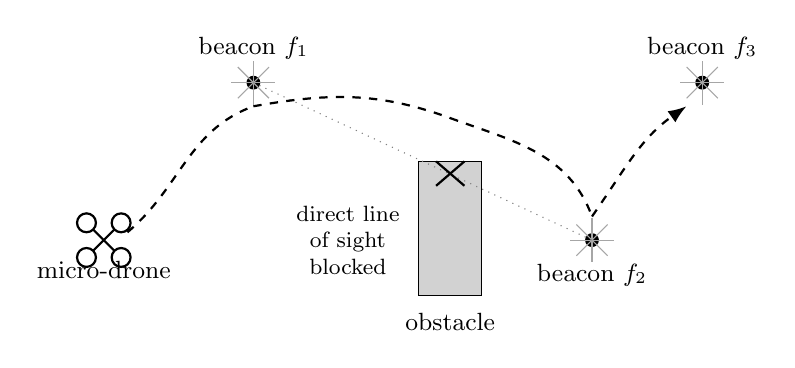
\begin{tikzpicture}[>=Latex, font=\small]
        % --- modulated light beacons ---
        \foreach \pos in {(2.3,3.0),(6.6,1.0),(8.0,3.0)} {
            \fill[black] \pos circle (2.5pt);
            \foreach \a in {0,45,...,315} { \draw[thin, gray!70] \pos -- ++(\a:0.28); }
        }
        \node[above=5pt] at (2.3,3.0) {beacon $f_1$};
        \node[below=5pt] at (6.6,1.0) {beacon $f_2$};
        \node[above=5pt] at (8.0,3.0) {beacon $f_3$};

        % --- obstacle, on the direct line from f_1 to f_2 ---
        \fill[gray!35] (4.4,0.3) rectangle (5.2,2.0);
        \draw (4.4,0.3) rectangle (5.2,2.0);
        \node[below=3pt, align=center] at (4.8,0.3) {obstacle};

        % --- blocked direct line of sight to f_2 ---
        \draw[dotted, gray] (2.3,3.0) -- (6.6,1.0);
        \draw[thick] (4.62,1.69) -- (4.98,2.00);
        \draw[thick] (4.62,2.00) -- (4.98,1.69);
        \node[align=center, font=\footnotesize] at (3.5,1.0) {direct line\\of sight\\blocked};

        % --- micro-drone at the start, top-down quadrotor ---
        \begin{scope}[shift={(0.4,1.0)}]
            \draw[thick] (-0.22,-0.22) -- (0.22,0.22);
            \draw[thick] (-0.22,0.22) -- (0.22,-0.22);
            \foreach \c in {(-0.22,-0.22),(0.22,0.22),(-0.22,0.22),(0.22,-0.22)} {
                \draw[thick, fill=white] \c circle (0.12);
            }
        \end{scope}
        \node[below=4pt] at (0.4,1.0) {micro-drone};

        % --- example mission path, detouring around the obstacle ---
        \draw[->, dashed, thick]
            (0.7,1.1) to[out=40,in=200] (2.3,2.7)
            (2.3,2.7) to[out=10,in=160] (4.8,2.55)
            (4.8,2.55) to[out=-20,in=110] (6.6,1.3)
            (6.6,1.3) to[out=55,in=215] (7.8,2.7);
    \end{tikzpicture}
    \caption{An illustration of the navigation task this thesis addresses. This is a schematic example, not a recorded flight path or the exact scene used in the experiments. A micro-drone must visit several light beacons in turn, distinguishing them by their modulation frequencies $f_1$, $f_2$, and $f_3$. An obstacle blocks the direct line of sight to beacon $f_2$, so steering toward the light alone is not enough to reach it. The drone must instead detour around the obstacle, which requires it to remember the light field rather than react only to the light it currently senses. The experiments in Chapters~\ref{chp:multibeacon} and~\ref{chp:obstacle} test the multi-beacon and obstacle cases separately.}
    \label{fig:task-concept}
\end{figure}

\section{Research Objectives}

This gap raises three questions, which this thesis addresses in turn:

\begin{enumerate}
    \item \label{rq:feasibility} Can such a drone carry the necessary light sensing on board and recover a reliable beacon signal in flight?
    \item \label{rq:multibeacon} Can it then navigate to several distinct light beacons in turn?
    \item \label{rq:obstacle} Can it navigate around an obstacle that blocks its line of sight to a beacon?
\end{enumerate}

The first question concerns feasibility: whether a board within the drone's mass budget can recover a reliable beacon signal during flight. The second and third concern capability: whether that sensing can then support the navigation the prior methods lacked, namely visiting several beacons in turn and routing around an occluding obstacle. The chapters\todo{A mention of chapters when we no longer mention the structure of the thesis. Remove/replace this!} that follow build the hardware and the controller that answer these questions, and test the result in simulation and in flight.

\section{Contributions}

To answer the research questions laid out in the previous section, this thesis makes four contributions.

First, it presents a custom photodiode sensing board that fits within a micro-drone's payload and size budget. It replaces an earlier Teensy-based prototype, which established the sensing principle but was too large and heavy to fly.

Second, it develops a fused navigation controller that combines the bearing with a gradient. The controller estimates the gradient from a map of the light field, which the drone builds from all eight photodiodes as it flies. The prior method instead estimated the gradient from a single photodiode, fitting a plane to the readings gathered along the drone's recent path, so its estimate depended on the drone's heading. Building the gradient on a map that all eight photodiodes populate removes this dependence, because the map holds a usable value at each location whichever way the drone faces. We choose the fitting method itself by comparing five candidate estimators on the same reference light field.\todo{This paragraph still feels a bit like it goes into to much detail. We should really only state the contributions here no?}

Third, it builds two navigation capabilities on this light map, which serves as the spatial memory the prior methods lacked. The first is multi-beacon traversal: because each beacon is modulated at a distinct frequency, the drone distinguishes the beacons in the map and visits them in turn. The second is obstacle avoidance: because the map records where the light was strong, the drone can route around an obstacle by following the stored field even while the beacon is occluded. A state machine ties these behaviours together, switching between the bearing, the gradient, and a blend of the two as each becomes reliable.

Finally, it validates the complete system in a Webots simulation and in real flight. The drone reaches several beacons in turn, and routes around an obstacle that blocks its line of sight to a beacon.

This thesis builds directly on the work of Huang et al.~\cite{huang2026lta}. That work provides the single-beacon bearing and gradient methods, the Webots simulator, and the lighter-than-air blimp platform. The fused controller, the map-based eight-photodiode gradient, the multi-beacon and obstacle-avoidance navigation, the photodiode board, and the CrazyFlie validation are the contributions of this thesis. In a later collaboration, Huang et al.\ mounted the same photodiode board and controller on their lighter-than-air blimp and reproduced the multi-beacon and obstacle-avoidance results.

\section{Thesis Overview}

The remainder of this thesis is organised as follows. Chapter~\ref{chp:background} reviews how drones navigate GPS-denied indoor spaces, motivates the choice of visible light, and introduces the prior algorithms of Huang et al. Chapter~\ref{chp:algorithm} analyses why those methods fall short under multiple beacons and occlusion, and designs the fused controller that overcomes them. Chapter~\ref{chp:hardware} presents the photodiode board and the payload, power, and size budget it must meet. Chapter~\ref{chp:realworld} describes the real-world implementation, including the signal pipeline that recovers each beacon from the noisy measured light. Chapter~\ref{chp:multibeacon} reports the multi-beacon experiments, and Chapter~\ref{chp:obstacle} the obstacle-avoidance experiments, in both simulation and real flight. Chapter~\ref{chp:conclusions} draws the conclusions, and Chapter~\ref{chp:futurework} sets out directions for future work.


% Create chapters
\chapter{Background \& Theory}
\label{chp:background}

\section{Visible Light Communication \& Sensing}

Visible light communication uses modulated light sources to transmit data, 
enabling a light source to serve simultaneously as illumination and a detectable 
navigation beacon.

\hlnotein{The spatial distribution of light intensity from a point source 
is described by the Lambertian model, which defines how intensity 
decays as a function of distance and angle from the source.}{Instead of dive into the Lambertian model,
I would instead just talk about it a bit, a more important point is that due to this Lambertian mode, 
how it affects or make other approach limited to multiple light overlapping to make it work.}

\hlnotein{Photodiodes convert incident light intensity into a measurable electrical signal, 
and their directional sensitivity makes them suitable for estimating the angle of incidence of a light source.}{I think this
paragraph can instad talk about what is the difference of our approach. What I mean is previous approach use light as
positioning system, our approach is more close to navigation system.}

\section{Bearing Angle Estimation}

\hlnotein{Prior work introduced a bearing angle estimation algorithm using a ring of 8 photodiodes 
that computes the relative angle toward a light source from the differential intensity readings across the array.}{No
need to talk about "8" phtodiodes here. more important thing is how to use sensor array to estimate the direction. 
Though we are almost the first one to do this with light, there are papers doing similar approach using other sensors.}

The bearing angle provides a single scalar direction toward the light source but 
contains no spatial information about the light environment; \hlnotein{when deploying multiple beacons,
their modulation frequencies must be chosen to avoid harmonic relationships, 
as the FFT cannot distinguish a frequency from its multiples.}{Too detail here, i would suggest to put it in the 
algorithm design. Here we are talking about more broader way of how to calcultae it. and the limitation.}

\section{Gradient-Based Source Seeking}

\hlnotein{Gradient-based source seeking navigates an agent toward a scalar field maximum by estimating and 
following the local gradient of that field.}{too compact, split to two sentences. this mean we will also spend a bit more
talking about this later.}

\hlnotein{Plane-fitting gradient estimation approximates the local gradient by fitting a least-squares plane 
to nearby light intensity measurements, yielding a continuous gradient direction without 
requiring deliberate perturbations.}{several terms is too detail to put here to explain how you make it work,
it should also be put later. at this point try to make it more easy for people to understand. something like
"by collecting the intensity overtime, a simple gradient estimation can be apply to estimate the direction of the light source.}

\hlnote{\section{Simulation Environment}}{I would put this more up, its ok if its short, but why we are using it? 
what is the advantage of using it? then talk about the good think about it.}

The simulation environment used in this thesis was developed in prior work and provides a physics-accurate Webots model of the 
drone platform with realistic light sensor simulation; for a full description the reader is referred to~\cite{}.

\chapter{Problem \& Algorithm Design}
\label{chp:algorithm}

\section{Why Existing Methods Fall Short}

The two methods this work builds on \hlnotein{each steer toward}{The grammar is weird. just say
The two methods, mentioning what two again. both demostrate sucessfuly navigation in the paper} a single light, 
but neither is enough for the navigation we \hlnotein{are after}{Don't write it like stuff we are after
write it the two methods fail}. The bearing points straight at the source and works well in open space, 
yet it has no memory of where the light is: the moment an obstacle blocks the line of sight, the drone 
is \hlnotein{left without a heading and cannot find its way around.}{Write it like this. Once the obstacle blocks
the line of sight, the drone immediately lose the signal and cannot determine the light direction. Thus, it loses
the direction to fine the way toward the light.} Following the light gradient with a single photodiode, 
as in prior work~\cite{huang2026lta}, \hlnotein{fares no better}{Write it more readable. the light gradient
approach also fail in tracking the light when it encounter a obstacle. }, since one sensor must infer the gradient 
from how its signal changes as the drone moves, which is slow and easily confused \hlnote{by noise.}{hmm im not really convinced
is the gradient really fail? i thought we use gradient to pull it away.}

\hlnotein{We study}{it jump directly into the simulation setup too fast. We need to first talk about why dont we
directly do the experiment in real-world to test it? there is multiple reason we can talk about. first, 
the real-world test will have ambient light noise. to first get rid of it we test it in simulation.
second, the simulation give fast repetitive experiment. again mention that here again to bridge reader easier.
} these methods in a Webots simulation that recreates the navigation task,
as Figure~\ref{fig:sim-setup} shows. The scene places a light source over the floor, 
an obstacle pillar in the path, and the drone to one side, so that the line of sight from 
the drone to the light is blocked \hlnotein{unless the drone first routes around the pillar.}{I dont feel necessary to mention
routes around the pillar here. just mentioned it will be blocked is enough.}
Every controller we compare in this chapter, the bearing-only and gradient-only baselines as well 
as the \hlnotein{fused controller}{Here the fused controller just pop out. you can mentioned we have our improved 
controller at the start. but dont bring up the detail term. just say. we tested A and B from Huang. and we show that they
all fail. and we further demonstrate our approach, which do A + B. works. you can mentioned a bit A + B here but dont jump
into detail.}, flies in this same scene from the same start position toward the same beacon, 
with identical sensing and flight settings, so that the only difference between the runs is the navigation 
method itself. The same environment also underlies the experiments of Chapter~\ref{chp:obstacle}.

\begin{figure}[h]
    \centering
    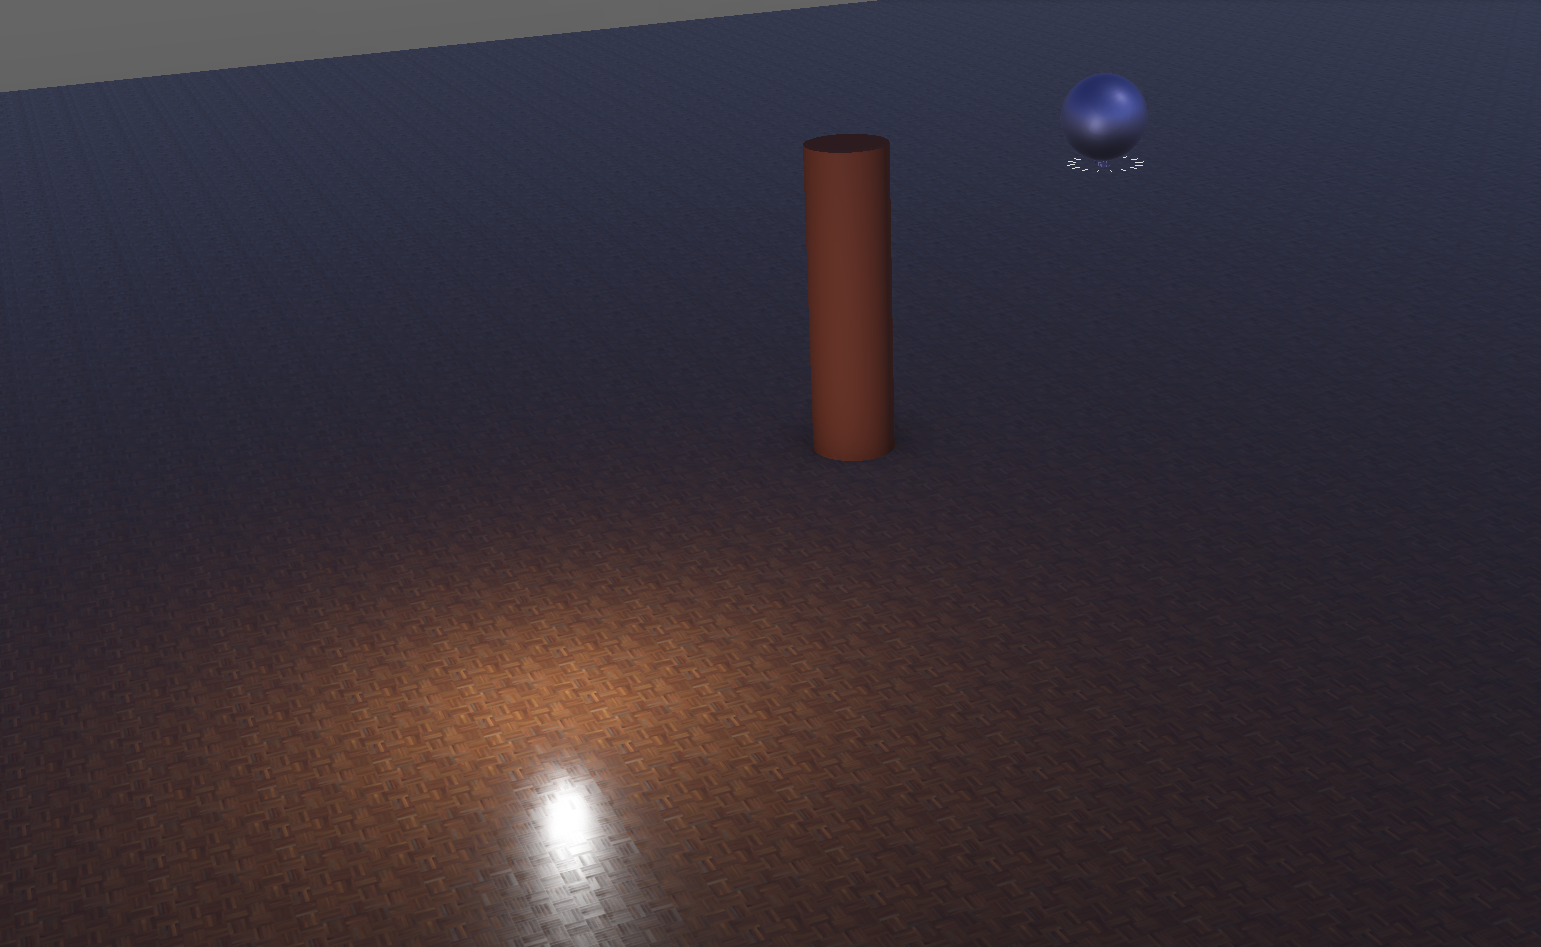
\includegraphics[width=0.6\textwidth]{figures/simulation_setup.png}
    \caption{The simulated test environment in Webots: a light source casting its pool of light on the floor, an obstacle pillar, and the drone approaching from one side.}
    \label{fig:sim-setup}
\end{figure}

In simulation, a bearing-only controller drives toward the light but, having no memory of the field,
cannot plan a way around the obstacle in its path and collides with the pillar, 
as Figure~\ref{fig:bearing-fail} \hlnotein{shows}{Its a long sentence. try to split it can talk
about each sentence more detail}. The collision is already a failure: on a real platform such 
an impact could damage the drone or the \hlnotein{obstacle}{BTW, I do test it myself in the simulation and see it crash
sometimes. but here in the graph it looks like it pass the obstacle? probably we need to make
some postprocess to make it mroe clear. should not be the graph show here}.

\begin{figure}[h]
    \centering
    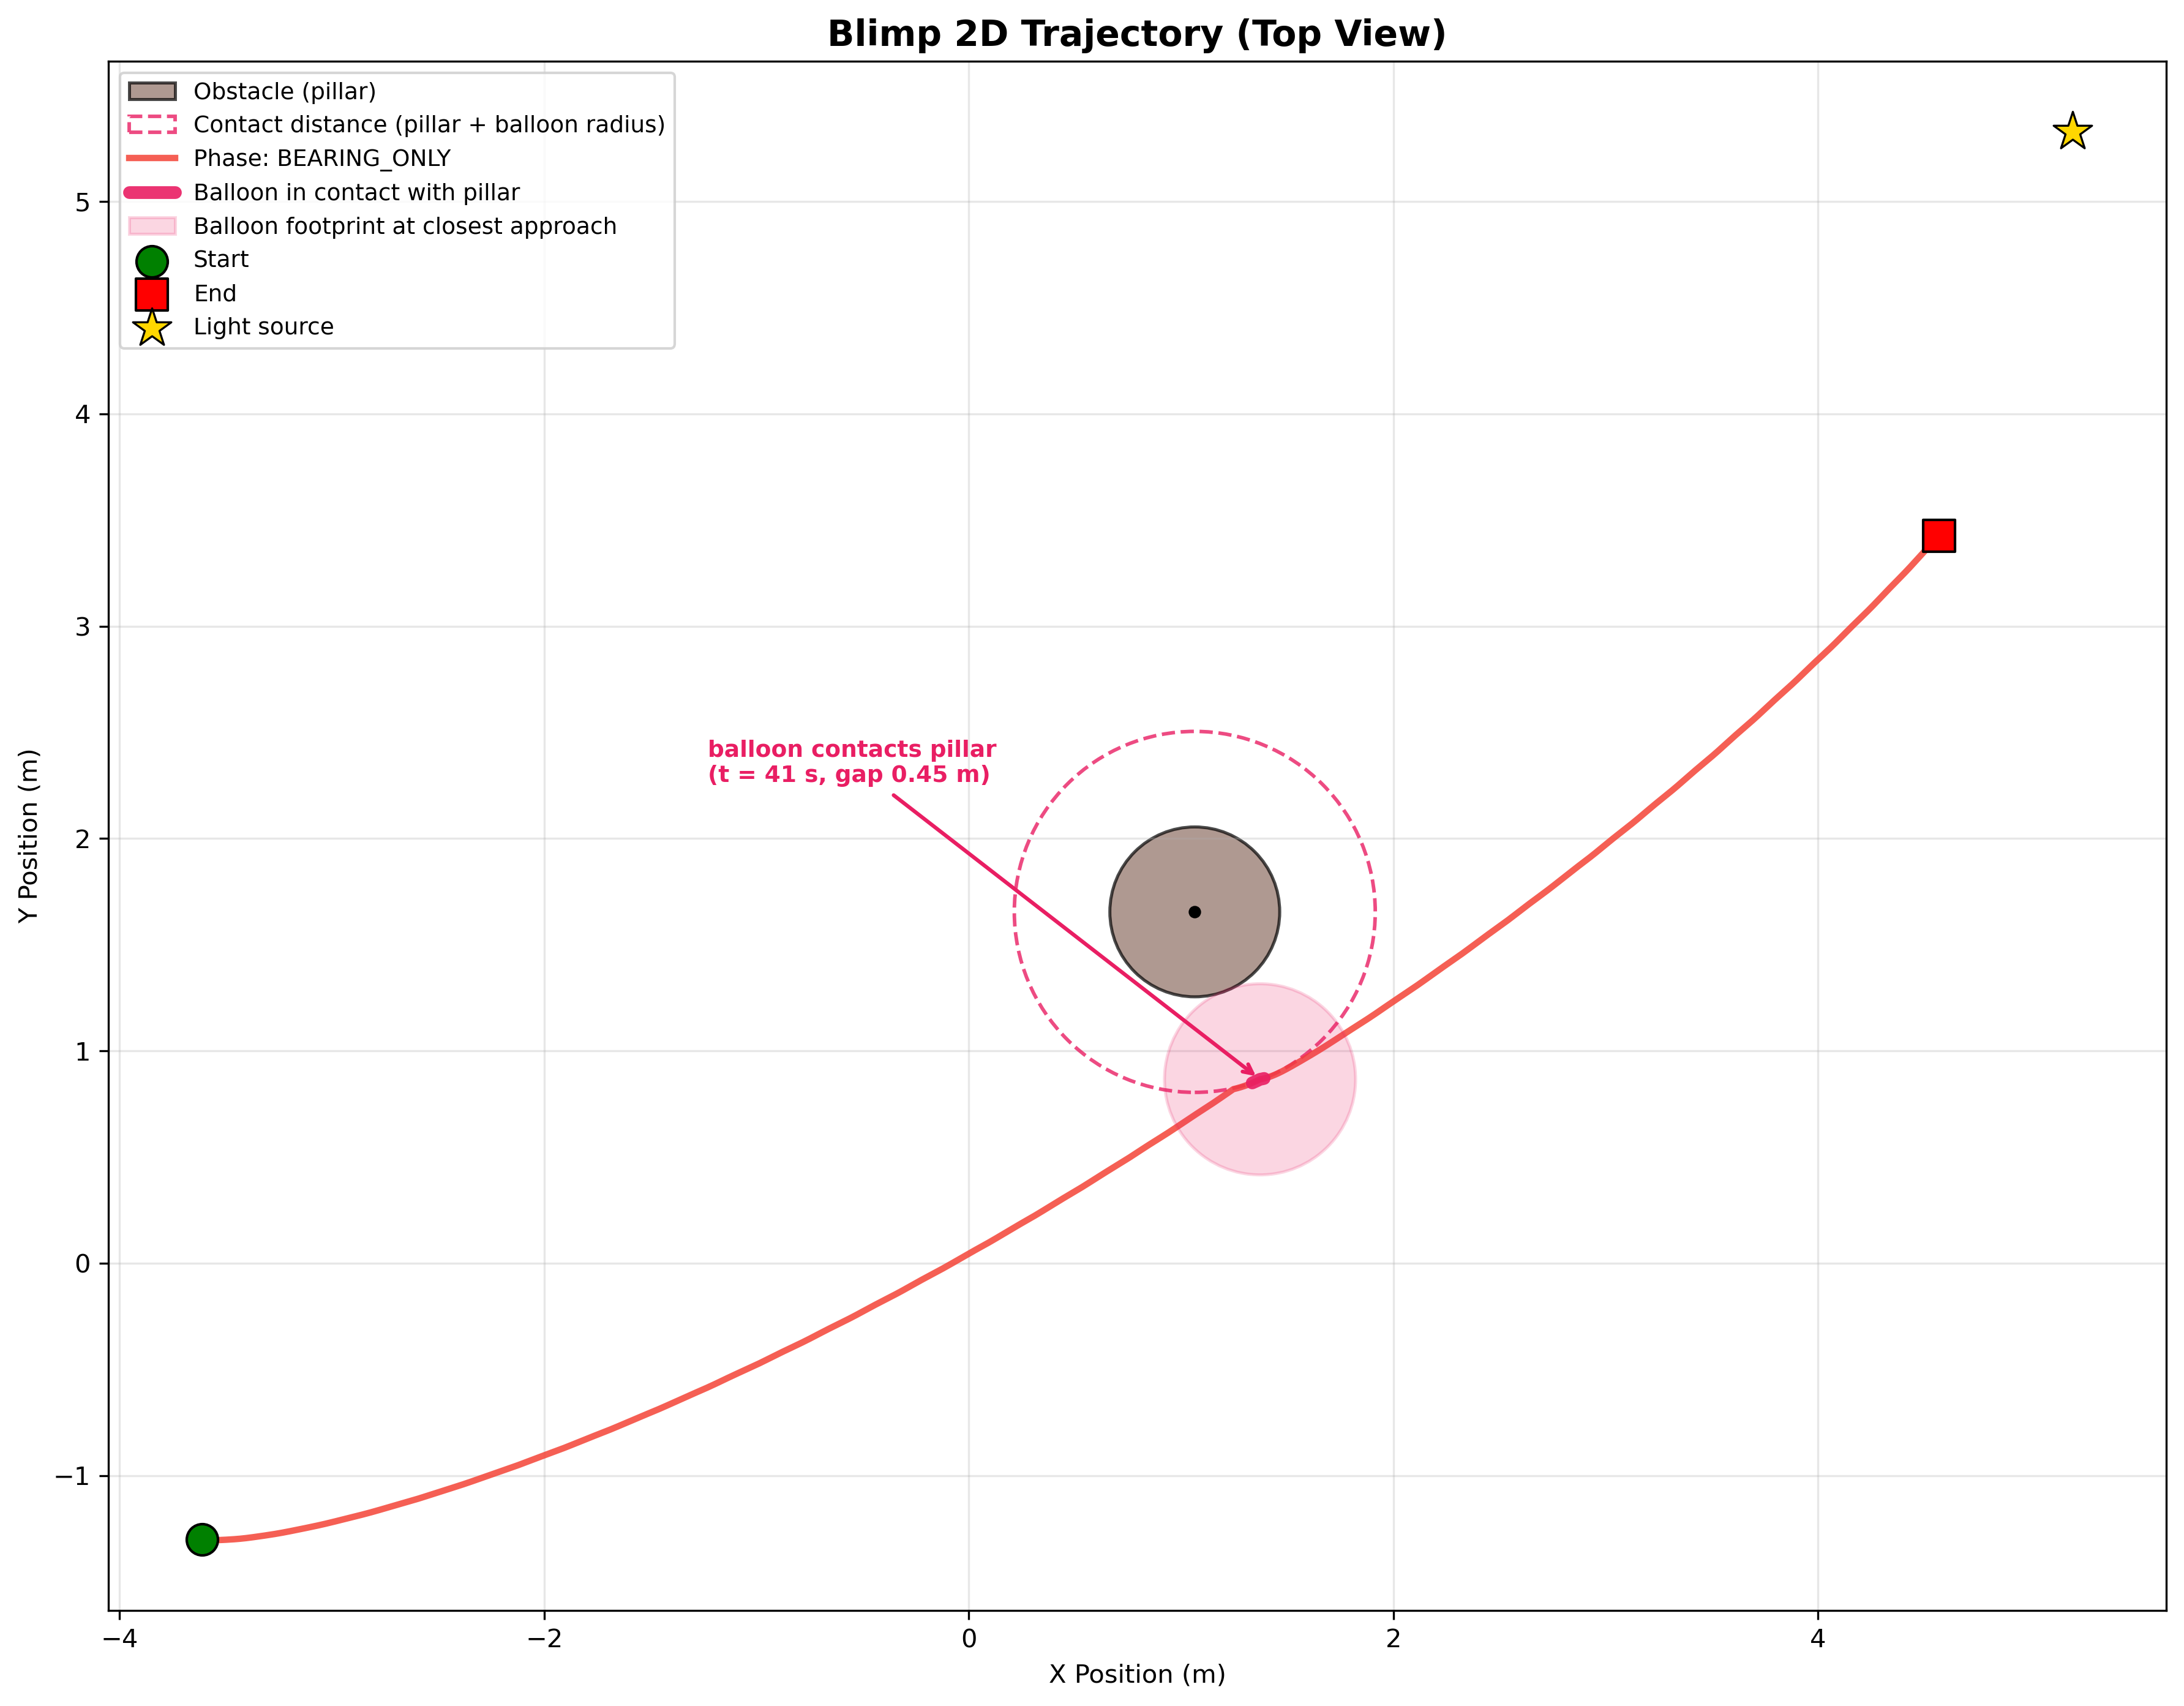
\includegraphics[width=0.6\textwidth]{figures/bearing_only_sim/blimp_trajectory_2d.png}
    \caption{Top-down trajectory in simulation: the bearing-only controller drives into the obstacle and cannot circle it cleanly, having no memory of the field to route around it.}
    \label{fig:bearing-fail}
\end{figure}

The single-photodiode gradient method struggles in 
the same setting: because it can only sense the gradient 
by moving, it follows a slow, wandering path that stalls 
at the obstacle rather than driving cleanly toward the source,
as Figure~\ref{fig:gradient-fail} \hlnote{shows}{This is good! explain a bit more
why it stall? What i understand is that the gradient will pull it away.}. Neither method, moreover, 
has any notion of more than one beacon, so reaching several lights 
in turn is out of reach from the start.

\begin{figure}[h]
    \centering
    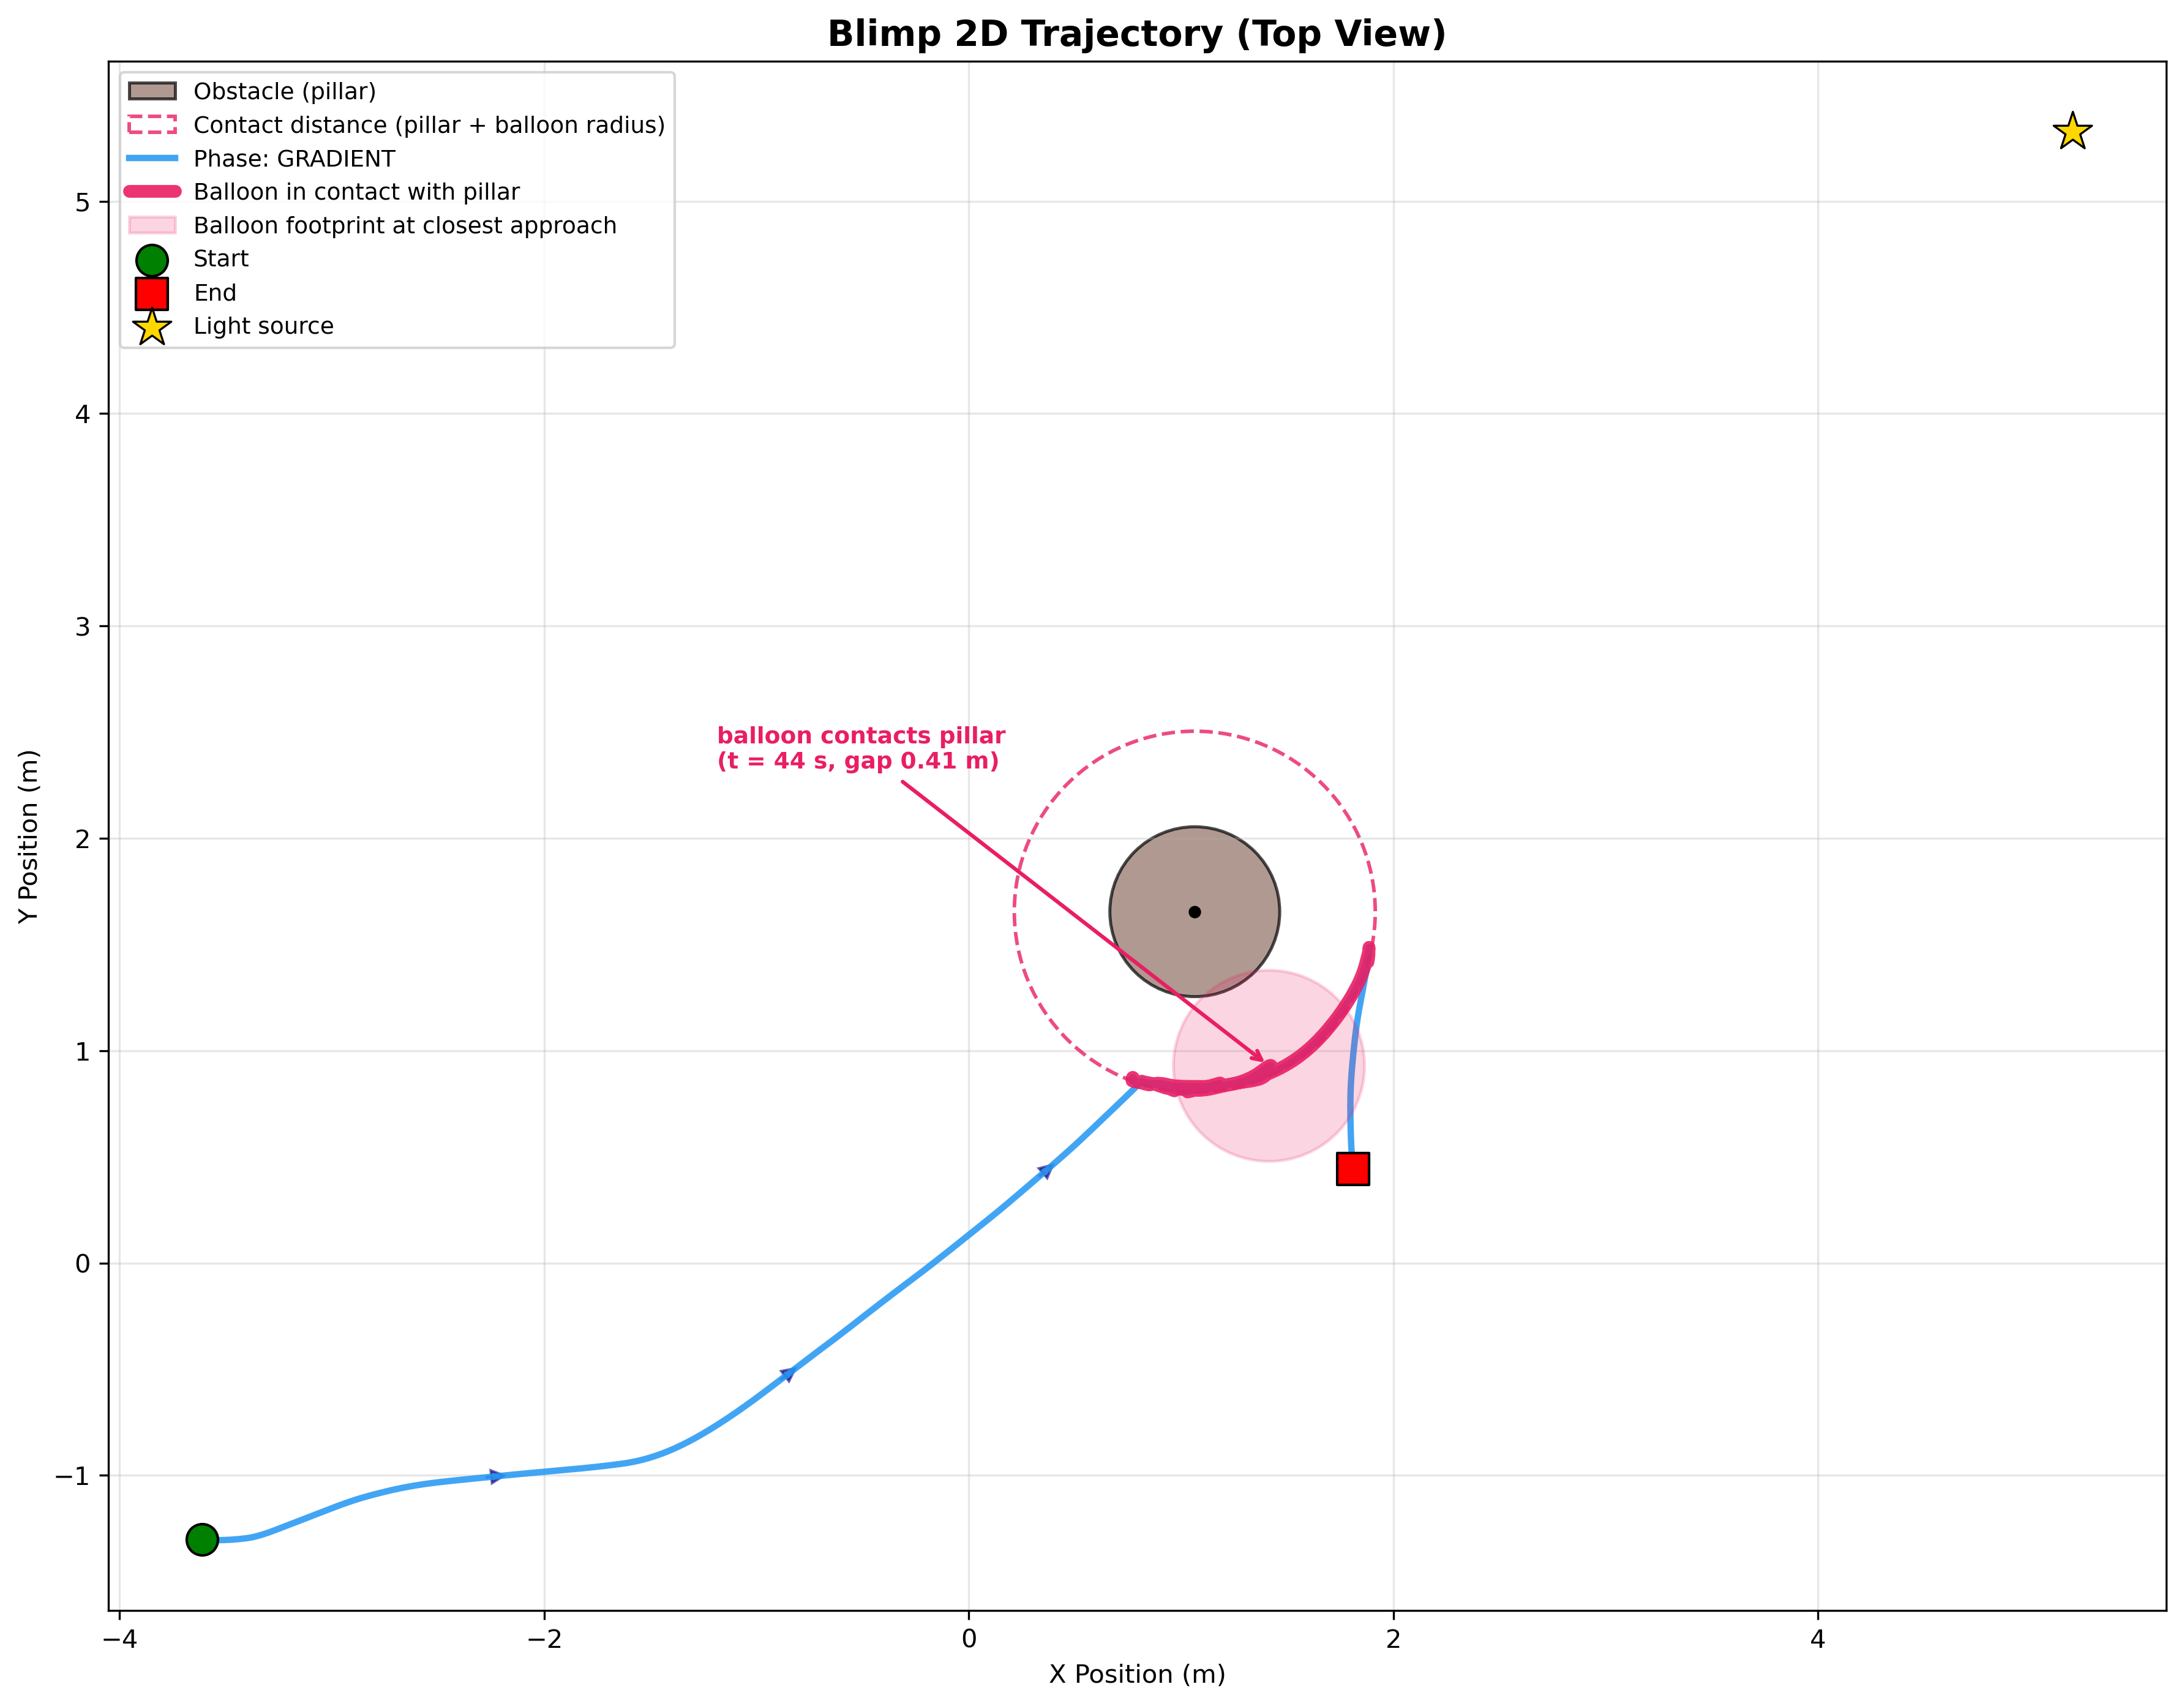
\includegraphics[width=0.6\textwidth]{figures/gradient_only_sim/blimp_trajectory_2d.png}
    \caption{Top-down trajectory in simulation: single-photodiode gradient ascent wanders and stalls at the obstacle, never reaching the light source.}
    \label{fig:gradient-fail}
\end{figure}

These shortcomings set \hlnote{the agenda for the rest of this chapter:}{For my preference
this sounds weird. i would go something like this. As demonstrated, the method proposed
by Huang encounter these shortcomings with both approach. This bring up the center problem in this
research. When there is a simple obstacle in the scene. How can we avoid the obstacle without introducing
extra sensor and complicated algorithm.} 
we develop a controller that fuses the two signals, estimates the
gradient from all eight photodiodes rather than one, and remembers
the light field in a map, so that it can route around \hlnotein{obstacles}{There is no
Why you come up with this. what do you see from the previous experiment for you to bring this up?
We need to bring up both pros and cons and then say that combining it is a good idea.} 
and visit multiple beacons. Its positive results are presented in 
Chapter~\ref{chp:obstacle}.

\section{System Overview}

To guide the drone toward a light beacon, we combine two inputs, both obtained from the same 
photodiode array. The first is a bearing angle that points straight at the source, which gives 
the controller an immediate heading whenever the beacon is in view. The second is a gradient direction, 
read from a map of the light field that the drone builds as it flies; this map records where the light is
stronger, so it stays useful even when the drone can no longer see the beacon directly.

Neither input is enough on its own. As the previous section showed, the bearing is fast but has no memory,
while the gradient is robust but only becomes available once the drone has built up a usable map. 
y combining them we get the best of both: the controller reacts quickly while the beacon is visible, 
yet keeps moving through a brief loss of signal by leaning on the map it has already \hlnotein{built}{this two paragraph
should be put before this}.

\hlnotein{Each update}{we move previous two more up. thus this need to rewrite. we should write it somthing like this.
Our system is aim to tackle a environment like this. in indoor environment where there is multiple
clusttering small obstacle. can we use single light for drone to navigate toward the light while having the 
ability to autonomously avoide the obstacle? and then with this task in mind. we need to achieve two thing. the 
drone need to move toward light efficiently enough -> means we need to use bearing. but also the obstacle avoidance
-> gradient. However, this bring up the problem. when should use use which. and then we bring it up there is a system design
with the state machine control} follows the same steps. \hlnotein{First, the per-sensor}{Lets try to make it more abstract.
This is an example. First the drone alway estimate the light direction using multiple photodiode weighting which we called bearing angle
. In the meanwhile, we collect the light intensity overtime and store them in a map. Where we further utilize this map
for gradient guidance algorithm. However, when there is two target from two algorithm, which one should we use ?
While instead of fully trust either, we propose a fusion model to combined the two} light signals of 
Section~\ref{sec:lightsignal} are turned into a bearing estimate and added to the light map. 
Then the local gradient is read from the map, and the bearing and gradient are merged into a single
target heading. A state machine decides how much to trust each input from the current signal
strength and map coverage, and walks the drone through search, alignment, approach and recovery
phases for each beacon in a multi-target mission, as summarised in Figure~\ref{fig:controller-overview}. The
controller finally outputs a target heading and a forward speed, which are passed to the drone's
own flight controller.

\begin{figure}[h]
    \centering
    \resizebox{\textwidth}{!}{%
    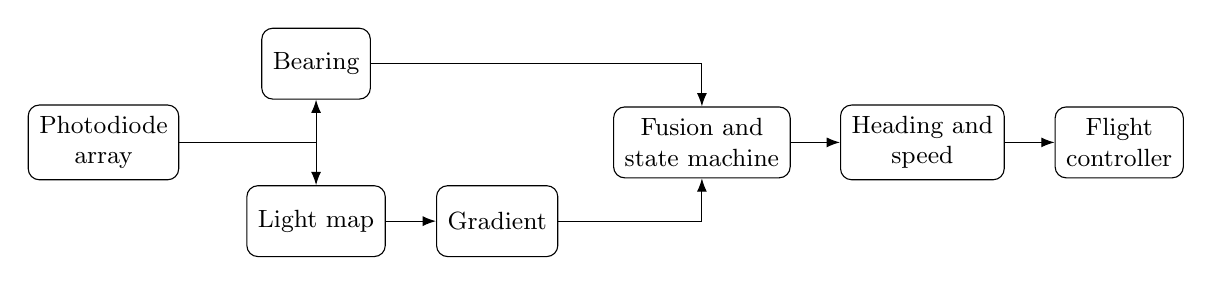
\begin{tikzpicture}[
        >=Latex,
        box/.style={draw, rounded corners, align=center, minimum height=9mm,
                    inner sep=4pt, font=\small}
    ]
        \node[box] (pd)      at (0,0)      {Photodiode\\array};
        \node[box] (bearing) at (2.7,1.0)  {Bearing};
        \node[box] (map)     at (2.7,-1.0) {Light map};
        \node[box] (grad)    at (5.0,-1.0) {Gradient};
        \node[box] (fuse)    at (7.6,0)    {Fusion and\\state machine};
        \node[box] (out)     at (10.4,0)   {Heading and\\speed};
        \node[box] (fc)      at (12.9,0)   {Flight\\controller};

        \draw[->] (pd) -| (bearing);
        \draw[->] (pd) -| (map);
        \draw[->] (map) -- (grad);
        \draw[->] (bearing) -| (fuse);
        \draw[->] (grad) -| (fuse);
        \draw[->] (fuse) -- (out);
        \draw[->] (out) -- (fc);
    \end{tikzpicture}}
    \caption{Overview of the fused navigation controller. The photodiode array feeds both a bearing estimate and a light map; the gradient is read from the map; the fusion and state-machine stage merges the bearing and gradient into a target heading and forward speed, which are passed to the drone's flight controller.}
    \label{fig:controller-overview}
\end{figure}

\section{Bearing Angle}

The first input to the controller is a bearing angle that points from the drone toward 
the light source. We obtain it from the bearing estimation algorithm of prior work 
by Harry Huang~\cite{huang2026lta}, which combines the relative light-signal magnitudes measured
 across the photodiode ring into a single direction; the full derivation is given in Section~\ref{sec:bearing}. This
gives the controller an immediate sense of where the beacon lies, without having to explore the environment first.

\hlnotein{Not every bearing can be trusted}{again try to elaborate more
try to do like this. However, Not ever bearing angle estimatione is accurate. For example, when the weighting 
is all zero, which represents there is no signal strength measured, the bearing angle will be random number instead of
pointing towards the light. Thus we need a value to score the confidence of the bearing estimation}, so each one comes 
with a measure of signal strength. We only act on a bearing when its strength is above a minimum threshold, 
which keeps the controller from chasing a heading that is really just noise from a weak, distant or absent 
beacon. \hlnotein{The bearings that do pass this check are then smoothed over time}{talk about why we smooth it. because it 
jitter still due not noise or due to sudden change is not favorable. there are multiple reasons why we want to smooth
it. but talk about it first and then speak about the smoothing method} with an exponential moving average, 
so that a single noisy frame does not cause an abrupt change of heading before the bearing reaches the fusion 
stage and the state machine. The update is
\begin{equation}
\hat{\psi}_B \leftarrow \hat{\psi}_B + (1-\beta)\,\Delta,
\label{eq:bearing-filter}
\end{equation}
where $\Delta$ is the wrapped angular difference between the new bearing and the current estimate $\hat{\psi}_B$, and $\beta$ controls how much of the history is kept.

\section{Multi-Beacon Traversal}

\hlnotein{A mission can involve several beacons, each modulated at its own frequency.}{It should be like this. A common application
might require several target anchors. To achieve this, we modulated multiple lights with different frequency} The drone 
senses all of them at the same time but visits them one after \hlnotein{another}{should be something like this. However,
When multiple light in the same environment. The drone can sense multiple light in the same time. To seperate each setpoint
for drone to traverse the targets accordingly we need to do the frequency analysis}. A single frequency analysis 
of the photodiode signal already contains every beacon's peak at once, so 
the sensing is fully parallel, as we show in Section~\ref{sec:freq-separation}; the controller then
picks one beacon as its current target, flies to it, and on arrival selects the next, so the \hlnotein{traversal 
itself is sequential.}{This is an example that passive term makes it not strong enough. It should be so we can traverse target.
Not something can \textit{traveral}}

What makes this possible is the frequency analysis at the heart of the sensing pipeline, introduced 
in Section~\ref{sec:lightsignal}. Each beacon blinks at its own rate, so taking an 
FFT of a photodiode's signal decomposes that signal into its frequency components, 
and every beacon then shows up as a separate peak at its own modulation frequency whose height reflects how 
strongly that beacon is seen. Because a single recording already contains every beacon's peak, we 
can read all of them from the same data rather than attending to one beacon at a time.

We must, however, choose these frequencies with care, because we modulate each beacon by switching its 
light on and off, which produces a square wave that carries strong energy not only at its 
own frequency but also at its odd harmonics~\cite{oppenheim1999dsp}. The frequency analysis 
itself separates a fundamental from its harmonics cleanly, since they fall in different bins; the 
danger is that if one beacon's frequency coincides with a harmonic of another, that harmonic deposits
energy in the wrong beacon's bin and the two become hard to tell apart. We therefore \hlnotein{space the modulation 
frequencies so that none lands on another's harmonics}{We therefore pick frequencies set that has minimum overlapping both
in their main frequency and the hormonic}, \hlnotein{a scheme we arrived at through a set of simple static
experiments on the Teensy platform.}{We first use a static board to retreive the best frequency pair.}

\section{Light Intensity Map}

As the drone flies, we build a spatial map of the light field that serves as the basis for
gradient-based \hlnotein{navigation.}{Again, try to rewrite this. first we need to talk about why. Thus it should be 
somthing like. Apart from the Bearing Angle Algorithm, we need to record the data overtime for gradient estimation.
Since we care more about the spacial distribution (talk about why), we make grid map.} We turn the environment into a regular grid, and
each cell records the strength of the light signal we measure as the drone
passes through it, \hlnotein{indexed by the drone's estimated position in a fixed world frame.}{I would skip explaining this}
\hlnotein{Using a grid keeps the map compact:}{Why we need to make it compact? lets reverse the later senteces.
First talk about the drift and what problem it will cause on the map. and then we try to update the latest in each map.} instead of storing every individual measurement,
we combine all the readings that fall within the same cell into one representative value,
so the size of the map depends on the area covered rather than on how long the drone has been 
flying. Because each reading is filed under the drone's estimated position, the map is only as trustworthy
as that estimate: drift in the position estimate would smear the recorded field across neighbouring cells and
blur the gradient we read from it. We assume the drone's onboard position estimate is accurate enough over the 
course of a mission for this smearing to stay small. We also limit how far the drift can accumulate: the map is 
not kept for the whole mission but reset whenever the drone switches from one beacon to the next, so it is always 
rebuilt afresh for the current beacon and any position error built up while chasing the previous one is discarded 
with the old map. 

The value we keep in a cell is the strongest light signal measured across the photodiode array 
at that location, using the per-sensor light signal defined in Section~\ref{sec:lightsignal}. When the drone
revisits a cell, we do not overwrite its value but blend it with the new measurement through an \hlnotein{exponential 
moving average,}{Again if you want to mentioned the moving average. its better to mentioned why? the reason can 
be that sometimes we observe some noise. but if there is no concrete reason. just skip it.}
\begin{equation}
I_{\text{cell}} \leftarrow \alpha\,I_{\text{cell}} + (1-\alpha)\,I_{\text{new}},
\label{eq:map-blend}
\end{equation}
which smooths out the short-lived fluctuations that occur as we sample the same location again over time. 
The smoothing factor $\alpha$ is set by default to weight the stored and new values equally; 
lowering it makes a cell follow new measurements more closely at the cost of more noise, 
while raising it gives a smoother but slower-adapting map.

The map therefore approximates a scalar field that rises 
toward the source, since the measured signal grows as the drone approaches the beacon, 
and this gives the drone a spatial memory of the light that the reactive bearing alone lacks. 
\hlnotein{Turning the field into a heading is the job of the gradient estimator described next.}{No, write it more like this
With a proximity to the light intensity map, we can then perform gradient estimation on this map. instead saying some task
is left.}

\section{Gradient Estimation}

\hlnotein{Gradient estimation gives the drone the direction it follows across the light map.}{The bearing angle
also gives direction. what is the difference. we need to pinpoint it precise here.}
Prior work inferred this direction from a single photodiode~\cite{huang2026lta}, reading the 
gradient from how that sensor's signal changed as the drone moved, which is slow because the 
drone must \hlnotein{keep moving to sense anything}{keep moving to collect the intensity data. not sensing 
anything}, \hlnotein{and fragile because one sensor sees the source only 
when it happens to face it.}{Should be, this approach can be fragile since it needs to make sure the
photodiode is facing the light target} The eight-photodiode ring avoids both issues: whichever way the drone 
is yawed at least one sensor faces the source, so its orientation no longer blinds the measurement,
and each location is captured directly rather than inferred \hlnotein{from motion.}{So we are doing 
difference, instead using 1 we are using 8. you point out the problem but the senstence end like we did not 
use it as a solution. so end it like. thus, we use 8 photodiode since it is less prone to the occlusion from
diffrence angle.}

\hlnotein{We estimate the gradient by fitting a plane to the map.}{start it like this. With the collected
light intensity map. we can thus estimate which direction the drone should mobe to increasing the 
light intensity fastest (something like this). To do this. we estimate the gradient direction
using the intensity map. For each cell in the intensity map} To the cells $\{(x_i, y_i, I_i)\}$ near 
the drone's current position we fit $I(x,y) = a x + b y + c$ by weighted least squares, weighting each 
cell by the inverse square of its distance to the drone so that nearer cells count for more, and we
take the gradient as $\mathbf{g} = (a, b)$; the controller steers along $\mathbf{g}$ whenever it 
navigates by the map. The same fit reports how \hlnotein{well the cells agree with the plane, through a weighted
coefficient of determination}{First talk about it can work. we need another paragraph or another seperate
sentence to talk about why we need this. For example. With give estimated direction, like the bearing angle,
it might be unstable and we need another something to determine the confidence of the estimation. and then we 
bring this up}
\begin{equation}
R^2 = 1 - \frac{\sum_i w_i\,(I_i - \hat{I}_i)^2}{\sum_i w_i\,(I_i - \bar{I}_w)^2},
\label{eq:gradient-r2}
\end{equation}
where $\hat{I}_i$ is the plane's value at cell $i$, $\bar{I}_w$ the weighted mean of the cell values, 
and $w_i$ the inverse-distance weights, which we use as a measure of how far the gradient can be trusted.

\hlnotein{This trust matters, because a gradient computed from too few cells, or from cells}{Yes this is good. but dont mention
it before mention it seperately here.} that do not fall on a \hlnotein{clean slope}{This needs more explanation,
what is clean slope? try to use more simple term to explain it and why it cause the estimation bad}, would point the drone
the wrong way. We therefore treat the gradient as reliable only when it is supported by at least a 
minimum number of cells, when its $R^2$ exceeds a threshold, and when its magnitude is 
\hlnotein{large enough to be meaningful;}{If it is possible. try to seperate different fail case. for example
what will happen if we have too few cell. give a more concrete example if possible} the specific values, together with the controller's other parameters, 
are listed in Appendix~\ref{app:parameters}. This is exactly the reliability the state machine refers to: 
until it is met the drone navigates on the bearing alone, and once it is, the gradient is blended into the 
heading or, \hlnotein{when the bearing is lost, followed on its own.}{try to seperate this. use two sentences to
talk about it. dont use too much connecting phrase if possible like \textit{and once it is}}

The gradient itself \hlnotein{can be estimated in more than one way}{I would write. Even though fitting a plane
is a well studied topic and there are multiple approaches proposed in literature. However, it is not clear
which approach best fit in our system.}, and the best choice is not obvious for the sparse, 
unevenly spaced cells of a real map. We therefore implement and compare five candidate methods: ordinary and
weighted least-squares plane fits~\cite{bjorck1996lsq, strutz2016wls}, a robust RANSAC fit~\cite{fischler1981ransac}, a 
local polynomial surface fit~\cite{bjorck1996lsq}, and finite differences~\cite{leveque2007fdm}. We judge them on three criteria, in order of importance: 
how often each returns a usable estimate, how accurately that estimate points, and how much computation it costs, since the method has to run on the drone's 
small microcontroller. Figure~\ref{fig:gradient-comparison} reports the first two for each method on a densely sampled reference map of the simulated light field.

We define these measures over a set of $N$ cells sampled across the reference map. 
At each cell a method either returns a gradient estimate that passes the reliability gates of the previous section or returns nothing; 
with $S_m$ the cells where method $m$ succeeds, its success rate is $|S_m| / N$. For each returned estimate $\hat{\mathbf{g}}_i = (\hat{a}_i, \hat{b}_i)$ we take the angular error 
against the direction straight to the source,
\begin{equation}
e_i = \left| \left( \hat{\theta}_i - \theta_i^\star + 180^\circ \right) \bmod 360^\circ - 180^\circ \right|,
\label{eq:angle-error}
\end{equation}
where $\hat{\theta}_i = \operatorname{atan2}(\hat{b}_i, \hat{a}_i)$ is 
the estimate's heading and $\theta_i^\star = \operatorname{atan2}(y_L - y_i,\, x_L - x_i)$ points
from cell $i$ to the source at $(x_L, y_L)$, and the wrap folds the unsigned
difference into $[0^\circ, 180^\circ]$. We discard cells within ten centimetres of 
the source, where the field is too steep to give a meaningful reference, and note 
that this straight-to-source reference is itself only approximate behind the pillar,
where the helpful direction leads around the obstacle rather than at \hlnote{it}{At it will
cause people lost like what. and this whole senstence also need to be split and try to give
more easier way to understand. If it is hard to explain in text. adding a graph will be helpful}. We
then average $e_i$ two ways: the own-coverage error over a method's own cells $S_m$, 
and the common-coverage error over the cells $C = \bigcap_m S_m$ that every method
estimates.

\begin{figure}[h]
    \centering
    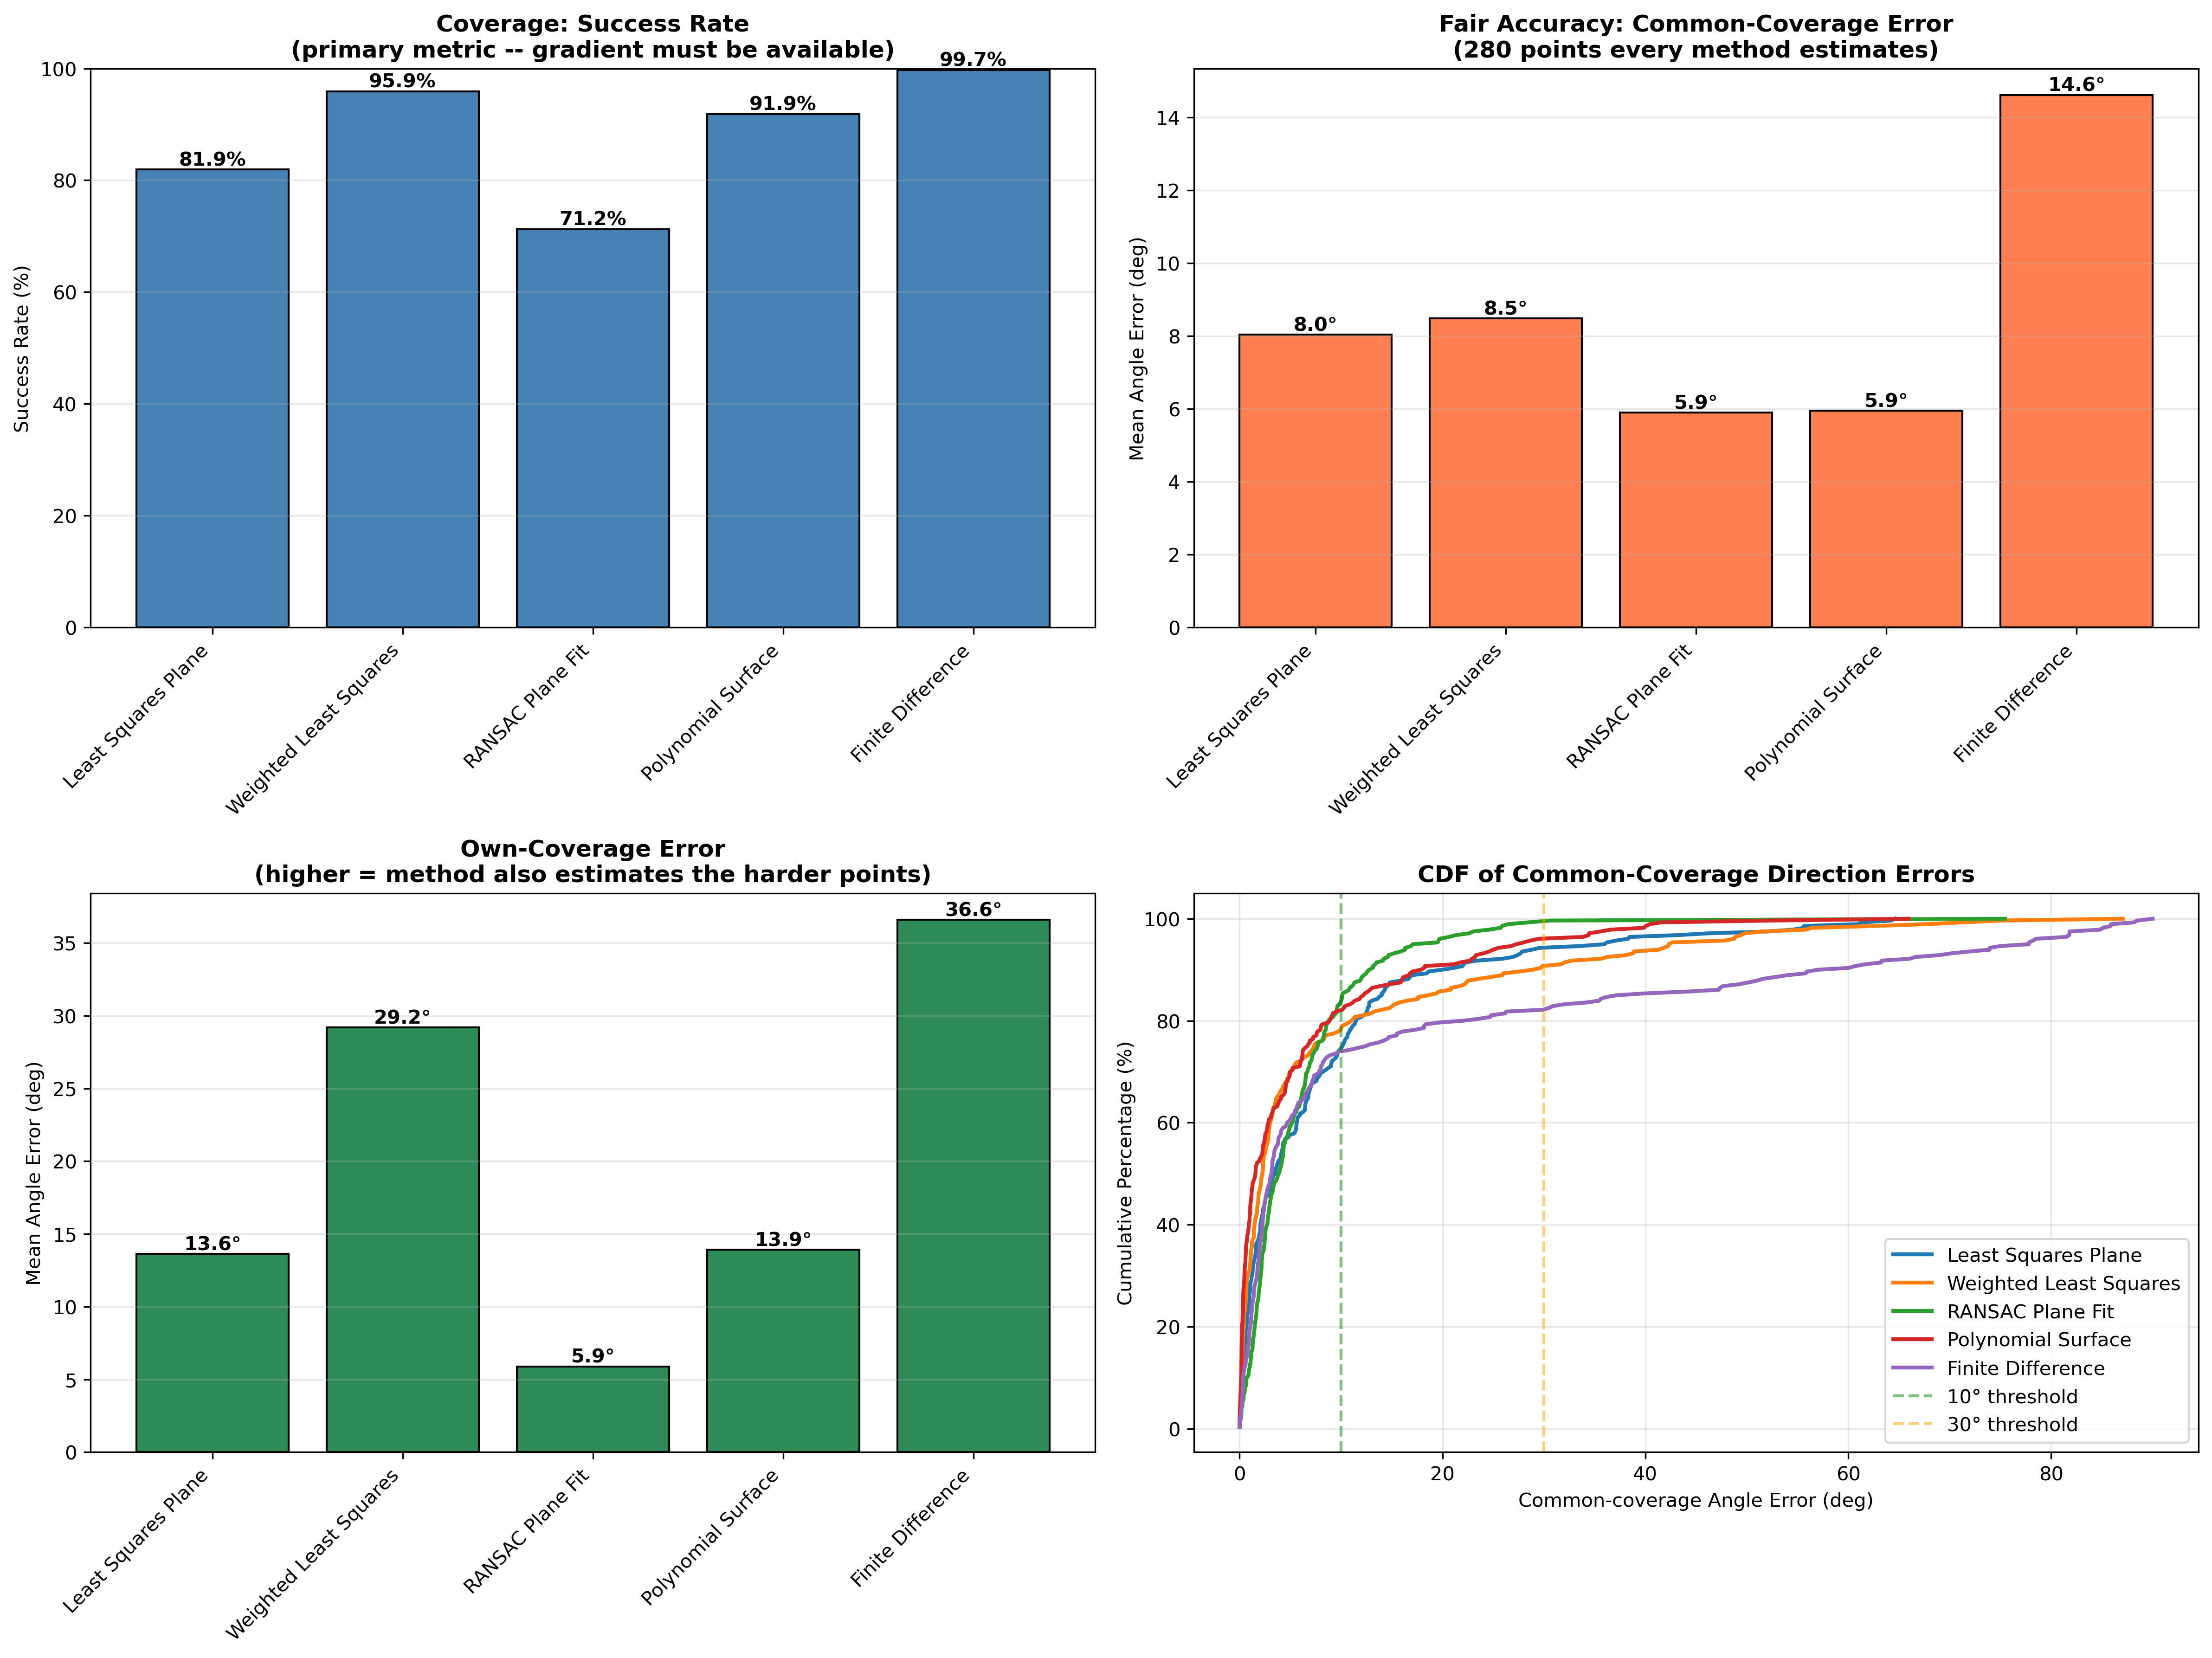
\includegraphics[width=0.85\textwidth]{figures/gradient_analysis/gradient_method_performance.png}
    \caption{Coverage and accuracy of the five gradient estimation methods on the reference map. Success rate is the share of points where the method returns a usable estimate. Accuracy is the angular error against the straight-to-source direction, reported both on the common set of points that every method estimates and on each method's own coverage.}
    \label{fig:gradient-comparison}
\end{figure}

Coverage is the criterion that matters most. The bearing already gives the
controller an accurate heading in open space, so the gradient 
does not have to be precise there; its job \hlnotein{is to be available wherever 
the drone is}{This needs to be rephrase. what does it mean wherever the drone is? I would
expect to read instead its improtant for drone to estimate the obstacle from the environment
at its current position. Have the ability to response at its current estimated location}, 
and above all when the bearing is lost behind an obstacle or 
between beacons. \hlnotein{A method that often returns nothing leaves the controller flying 
blind at exactly those moments.}{Also a bit confusing about what does this conveying. give
more specific example for context} \hlnote{Finite differences}{Add a method or algorithm behind
this so people know you are refering to previous several choices} return an estimate almost always,
at \hlnote{99.7\%}{What is this number meaning? Again this indicating the coverage needs
to be explain in a more easy way to understand}, but from so few cells that the 
direction is noisy; RANSAC succeeds least often, at 71\%, discarding too many cells 
as outliers; and the plane and polynomial fits sit between. Weighted least 
squares returns a usable estimate 96\% of \hlnotein{the time, second only to the 
noisy finite differences.}{I like the inspection and the analysis you tried to do here
But this really needs to rewrite. I will speak to you in detail to understand this part more}

The raw angular error, by contrast, is a misleading way to rank the 
methods, because it is entangled with coverage. A method that 
quietly fails on the hardest cells is never charged for them, 
so its average error flatters it, while a high-coverage method like 
weighted least squares is scored everywhere, including the cells right
under the elevated source where the measured field bends sharply
and behind the pillar where it leads around the obstacle rather than
straight at it. This shows directly in the figures: on its own coverage
weighted least squares records a mean error of 29 degrees, against 5.6 degrees
for the low-coverage RANSAC fit. When we instead score every method on the
same common set of cells, the cells that all of them estimate, the gap nearly
closes. The plane, polynomial, RANSAC and weighted least-squares fits then 
agree to within about three degrees, from 5.6 to 8.5 degrees of mean error,
with only finite differences staying noticeably noisier at 14.6 degrees;
weighted least squares itself falls from 29 to 8.5 degrees, which shows
that most of its apparent inaccuracy was simply the price of estimating
the difficult cells the other methods decline. The remaining differences
of a few degrees are not decisive: the bearing compensates them in open
space, and the steep field under the source would not even appear in
flight, where the drone follows a partial map and never measures that
drop.

\hlnote{Too complex}{Its fine to dig into detail here. but we need a major
refine of this. I think we need to put subsection in this section to first talk
about the setup, which is done good at first. And then subsection about different
method. and then subsection detail about the critirion that you are interested in. 
And then last subsection we compare them}

\begin{figure}[p]
    \centering
    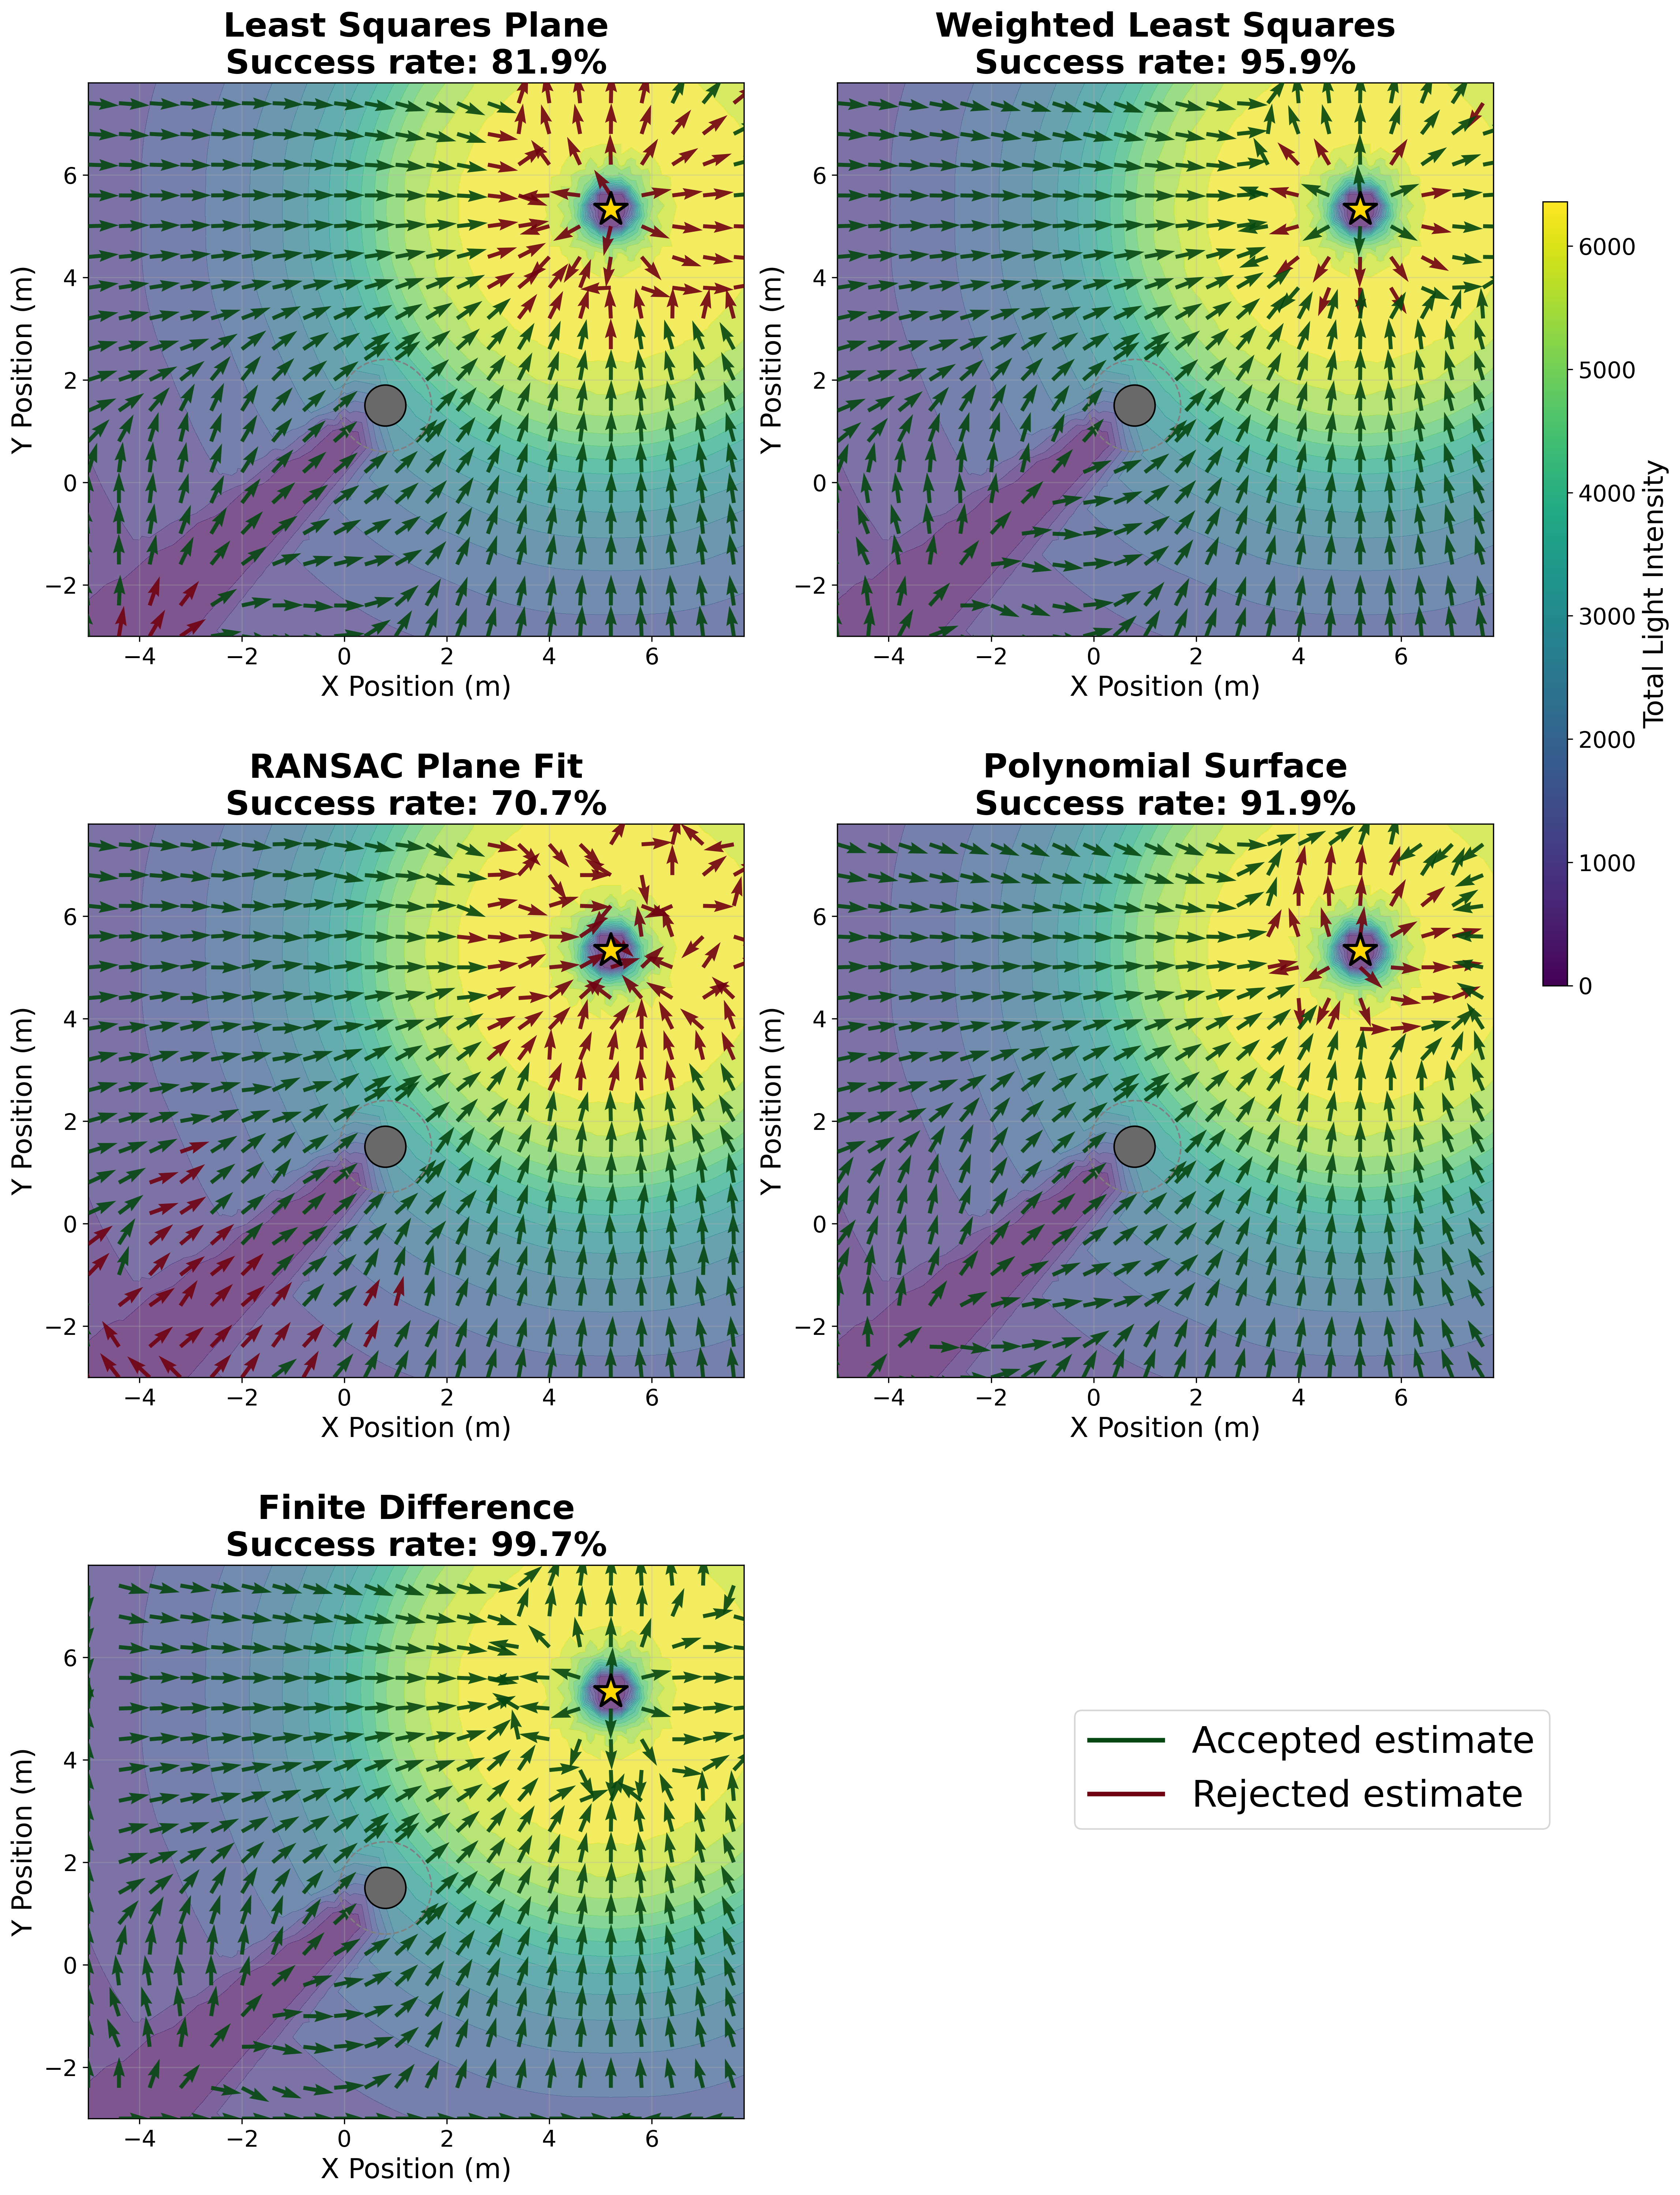
\includegraphics[height=0.86\textheight]{figures/gradient_analysis/gradient_method_comparison.png}
    \caption{Estimated gradient directions across the field for each method, coloured by angular error against the straight-to-source direction. The grey disc is the obstacle and the dashed circle the clearance the drone keeps. The large errors cluster under the source and behind the obstacle, where the field bends and pointing straight at the source is no longer the useful direction.}
    \label{fig:gradient-directions}
\end{figure}

Computational cost and robustness settle the choice. Weighted least squares 
solves one small fixed-size linear system whose runtime is the same on every call,
which sits comfortably within the budget of the drone's microcontroller, and its
inverse-distance weighting makes it robust to the changes in overall light level
that occur as the drone moves nearer to or further from the source. RANSAC, the
most accurate method on its own coverage, is the most expensive and the least
predictable, since it repeatedly fits and scores random subsets and its running
time varies from call to call, which is awkward for a real-time control loop on
a small processor. Finite differences are the cheapest but the noisiest.
Weighted least squares therefore offers the best combination for this platform:
the highest usable coverage, a low and constant computational cost, and
robustness to light-level changes, which is why the controller estimates
its gradient this way.

\section{Controller State Machine}

\hlnotein{A state machine governs what the drone does at each moment of a flight, 
since the bearing and gradient tell it which way to go but not what to do.}{1. state 
machine governs i understand 2. algorithm guide it where to go i understand. but what does 
it mean what to do?} It moves the drone through a small set of navigation phases, runs 
through them once for every beacon in the mission, and governs when the drone 
may rely on the map instead of the bearing, as Figure~\ref{fig:state-machine} \hlnotein{shows.}{
    again please clearly state the challenge first. here we should first write somthing like this.
    While combining the bearing angle and gradietn method can do something when it is exposed
    under sufficient light signal, when the light is block or simply out of field of view, or
    anything you come up with, the algorithm immediately fail. Second problem when drone is moving
    when do we need to trust the bearing and when is the gradient. list these problem first. and then
    bring up the state-machine to solve this
}

The drone starts in a searching phase, where it has no usable bearing or 
gradient yet. Here it slowly rotates in place to sweep the photodiode 
ring across the room until a beacon comes into view, and as soon as a
bearing arrives with enough signal strength to be trusted, the drone
moves on to aligning.

\hlnotein{In the aligning phase the drone turns toward the target without 
flying forward,}{So what we need to do here is first clarify what different stage is
and why? I know the graph might already show it. but we still need to write about it in
the context.} so that it is pointing roughly the right way before 
it commits to moving. Once its heading is within a small tolerance of 
the target it switches to approaching and begins to fly forward, correcting
its heading continuously as it goes. If it later drifts too far off heading,
it drops back to aligning.

Throughout aligning and approaching, the heading the drone follows 
is not the bearing alone. \hlnotein{While the map is still sparse the drone steers by 
the bearing, but as soon as the gradient becomes reliable the controller 
blends it into the heading, so the drone is already using both inputs together
well before it would ever need to fall back on the map by itself.}{I feel like here
is some grammar issue. for example->While the map is stil..., but as soon as..., I feel
like we are trying to say two things here? Please split this sentence and give more detail}

\hlnotein{The drone knows it has arrived when the signal strength climbs above an arrival 
threshold}{Bring this up like this. While now the drone can successfully move to the 
target, the drone needs to determine whether it reaches the target. and then we talk about the threshold.
and what threshold here trying to say? again bring up the intensy will increase and thus we can use it}, 
which only happens 
close to the beacon. The arrival threshold can be
tuned for different beacons or circumstances. It then enters a dwelling phase,
holding its position for a short, configurable time before moving on to the
next beacon and starting the cycle again. When the last beacon has been reached,
the mission is complete.

\hlnotein{The recovering phase is what keeps the drone moving when the beacon disappears, 
for example}{bring the example first, and then say we need the revoering} when 
an obstacle comes between the drone and the light and a purely 
\hlnotein{reactive controller would be stuck}{hard to understand what do you mean
reactive and what is \textit{stuck}}. If the bearing is lost but the gradient map 
is still reliable, the drone enters this phase and keeps flying forward on the 
gradient direction alone, climbing the stored light field to work its way out of 
the shadow. As soon as the beacon comes back into view it returns to approaching,
and only if the map itself becomes unreliable does it fall back to searching.

\begin{figure}[h]
    \centering
    \resizebox{\textwidth}{!}{%
    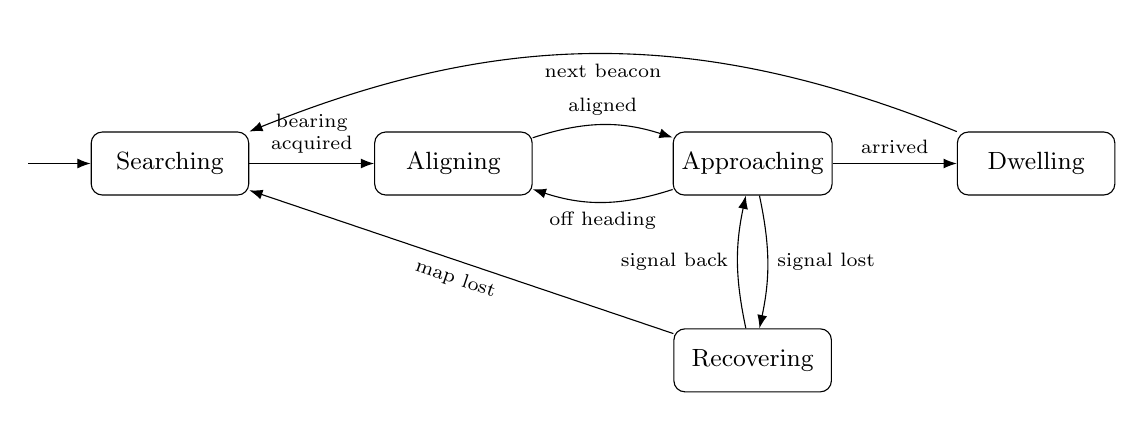
\begin{tikzpicture}[
        >=Latex,
        st/.style={draw, rounded corners, align=center, minimum height=8mm,
                   minimum width=20mm, inner sep=3pt, font=\small},
        lbl/.style={font=\scriptsize, align=center}
    ]
        \node[st] (S)  at (0,0)     {Searching};
        \node[st] (AL) at (3.6,0)   {Aligning};
        \node[st] (AP) at (7.4,0)   {Approaching};
        \node[st] (DW) at (11.0,0)  {Dwelling};
        \node[st] (RE) at (7.4,-2.5){Recovering};

        \coordinate (start) at (-1.8,0);
        \draw[->] (start) -- (S);

        \draw[->] (S) -- (AL) node[midway,above,lbl]{bearing\\acquired};
        \draw[->] (AL) to[bend left=18] node[midway,above,lbl]{aligned} (AP);
        \draw[->] (AP) to[bend left=18] node[midway,below,lbl]{off heading} (AL);
        \draw[->] (AP) -- (DW) node[midway,above,lbl]{arrived};
        \draw[->] (AP) to[bend left=12] node[midway,right,lbl]{signal lost} (RE);
        \draw[->] (RE) to[bend left=12] node[midway,left,lbl]{signal back} (AP);
        \draw[->] (RE) -- (S) node[midway,below,lbl,sloped]{map lost};
        \draw[->] (DW) to[bend right=22] node[midway,below,lbl]{next beacon} (S);
    \end{tikzpicture}}
    \caption{Navigation state machine, run once per beacon. The drone searches for the beacon, aligns its heading, then approaches while correcting; it dwells briefly on arrival before moving to the next beacon, and enters recovering to follow the gradient map alone when the bearing is lost behind an obstacle.}
    \label{fig:state-machine}
\end{figure}

\section{Control Output}

The controller's main output is a single target heading, formed by merging the 
bearing direction $\psi_B$ and the gradient direction $\psi_G$. Because both are angles,
we combine them with a weighted circular mean~\cite{mardia2000directional},
\begin{equation}
\psi = \operatorname{atan2}\!\big(w_B \sin\psi_B + w_G \sin\psi_G,\; w_B \cos\psi_B + w_G \cos\psi_G\big),
\label{eq:fusion}
\end{equation}
rather than a \hlnotein{plain average, which would suffer wrap-around errors near 
0 and 360 degrees.}{What does it mean wrap-around errors?} \hlnotein{When both inputs are 
reliable we set $w_B = w_G$, weighting }{Lets break this into more detail. So list several
case that is possible \textit{first} and then how we do corresponding to it.}
them equally; when only one is available its weight is one and the other zero; 
and when neither is, the drone holds its current heading. With these fixed, 
equal weights the combination is closer to a gated hand-off than to a continuous,
confidence-weighted fusion: where both signals overlap the heading is simply their
bisector, and the rest of the time the controller acts on whichever signal the
state machine deems reliable, the bearing in open space and the gradient behind
an obstacle. We keep this simple and predictable form here; letting $w_B$ and $w_G$
scale with a per-signal confidence is a natural extension we leave to future work.

\hlnotein{Alongside the heading, the controller sets a forward speed. The drone only flies
forward once it is roughly pointing at the target, so the speed is held
at zero while it is still turning to align and set to a fixed cruising 
speed once it is aligned and approaching. This keeps the drone from 
drifting sideways while it corrects a large heading error.

The heading and speed are handed to the drone's own flight controller
as setpoints, while the altitude is held at a fixed height throughout.
The controller therefore commands the drone in the horizontal plane only,
leaving the low-level work of stabilising the drone and holding altitude 
to the flight controller beneath it.}{Things like this can be shorten. since people
dont know what do you mean \textit{low-level}. discribing it like a simple robot.
what we are doing here is we want to find the best heading. thus we tried to dixed
the speed for the drone and the height is also predetermine. We can mentioned things like
horizontal plan only but what is the insight about this? probably the bad side? 
we need to bring up \textit{Why we want to mention it here?} if its hard to explain or
too long, just make it simple}

\chapter{PCB Hardware Design}
\label{chp:hardware}

\section{The Original Prototype}

The bearing and gradient algorithms were first realised on an earlier prototype built around a Teensy~4.1 microcontroller, which read the photodiodes correctly but was far too large, heavy, and power-hungry to fly on a micro-drone, and carried far more compute than the algorithms require.

The original board used larger, ready-made photodiode and operational-amplifier modules and provided space for sixteen photodiodes, more than the eight that Harry's prior research showed to be sufficient (Figure~\ref{fig:old-prototype}).

\begin{figure}[t]
    \centering
    \missingfigure[figwidth=0.6\textwidth]{Photograph of the original Teensy 4.1-based prototype board}
    \caption{The original Teensy 4.1-based prototype board.}
    \label{fig:old-prototype}
\end{figure}

This chapter presents a redesigned board that keeps the same sensing principle while meeting the size, weight, and power limits of the CrazyFlie platform, and compares the new design against this original throughout.

\section{Design Requirements}

The new board was designed to correct the shortcomings of the original prototype while meeting the CrazyFlie~2.1's hard limits: a total mass below 13 grams and a maximum diagonal footprint of 44\,mm.

It therefore uses eight photodiodes rather than sixteen, compact surface-mount photodiode and amplifier components in place of the larger ready-made modules, and offloads all computation to the CrazyFlie so that no power-hungry on-board microcontroller is required.

\section{Circuit Design}

Eight photodiodes are arranged in a ring and each connected to a transimpedance amplifier that converts the photodiode's current output to a measurable voltage signal.

The voltage outputs are digitised by an ADC module that communicates with the CrazyFlie's onboard processor over SPI, providing all eight channel readings at each sample.

The board includes optional first-order filter pads at each channel, allowing a low-pass or high-pass filter to be populated depending on the noise characteristics of the deployment environment.

\section{PCB Layout}

The eight photodiodes are uniformly distributed at 45\textdegree{} intervals around the full 360\textdegree{} circumference of the board to provide symmetric angular coverage.

A ground plane is included in the PCB layout to reduce the impact of electromagnetic interference generated by the drone's motors on the photodiode signal readings.

Before integration with the drone, the assembled board was verified to produce correct voltage readings on all eight channels using a standalone Teensy microcontroller.

\chapter{Simulation Experiments}
\label{chp:simulation}

\section{Experimental Setup}

The simulation experiments are designed to probe the central challenges of single-light navigation: navigating around obstacles, and recovering a reliable gradient from the sparse measurements gathered along a flight path, which first requires that the light field forms a navigable gradient at all.

All experiments share a single setup in the Webots environment described in Chapter~\ref{chp:background}: a single overhead light source with a known position serves as the navigation target, providing a controlled setting in which each challenge can be isolated and tested (Figure~\ref{fig:sim-setup}).

\begin{figure}[t]
    \centering
    \missingfigure[figwidth=0.6\textwidth]{Webots simulation setup --- single overhead light source, drone start pose, and obstacle placement}
    \caption{Shared simulation experiment setup used across all simulation experiments.}
    \label{fig:sim-setup}
\end{figure}

\section{Experiment 1: Baseline Bearing-Only Navigation}

\textit{Question: how does the bearing-only controller behave in open space and in the presence of obstacles?}

The bearing-only controller navigates successfully toward the light source in unobstructed conditions but fails to navigate around obstacles, as it has no spatial memory of the light environment and cannot recover a path once line-of-sight is disrupted.

\section{Experiment 2: Dense Probe Map Collection}

\textit{Question: does the light intensity field form a navigable gradient, and what does it look like under ideal sampling conditions?}

A systematic grid scan produces a dense probe map of the light intensity field, confirming a consistent gradient toward the source and providing an ideal-coverage reference dataset for evaluating gradient estimation methods.

\section{Experiment 3: Gradient Estimation Method Comparison}

\textit{Question: which of the five gradient estimation methods most accurately recovers the gradient direction from the dense probe map?}

The five candidate gradient estimation methods introduced in Chapter~\ref{chp:algorithm} are evaluated against the dense probe map, with weighted least squares yielding the lowest directional error.

\textit{Question: how does gradient estimation quality degrade when the drone can only use the map points visited along its flight path?}

Gradient quality is re-evaluated using only the flight-path-visited subset of map points, quantifying the accuracy penalty of the realistic sparse coverage scenario compared to the ideal full-map case.

\section{Experiment 4: Fused Controller Validation}

\textit{Question: can the fused controller navigate around obstacles that the bearing-only controller cannot handle?}

The fused controller is validated in simulation by demonstrating successful navigation around an obstacle, with the state machine correctly transitioning through modes as the drone's map coverage and bearing signal quality evolve.

\chapter{Real-World Implementation \& Experiments}
\label{chp:realworld}

\section{Sim-to-Real Adaptation}

\hlnote{The primary adaptation from simulation to the real world}{I would do this instead. not speaking about
the sim to real adaptation, just talk about real world implementation challenge} is the switch from raw light intensity to SNR at the modulated beacon frequency, which isolates the target light 
from ambient sources and background illumination.

A 500\,Hz hardware low-pass filter is populated on the PCB to prevent motor noise
and reflection artefacts---which occur at frequencies above the Nyquist limit of the ADC---from 
aliasing into the FFT and corrupting the SNR estimate.

Beyond the base algorithm's existing DC removal and Hamming window, three additional filters were introduced: block-based estimation, noise floor estimation, and per-channel magnitude IIR filters, to improve signal stability during flight.

\section{Experimental Setup}

\hlnote{Real-world experiments}{its better to split this to two cases and talk about the expriment} are 
conducted with two modulated light beacons positioned in a room, 
with the CrazyFlie~2.1 carrying the custom photodiode PCB as the sensing payload.

\section{Experiment 5: Filter Validation}

\textit{Question: do the additional filters improve signal stability during flight compared to the base algorithm alone?}

Raw signal recordings with and without the block estimation, noise floor estimation, and IIR filters applied are compared, demonstrating the reduction in noise and signal variance achieved by each filtering stage.

\section{Experiment 6: SNR Field Mapping}

\textit{Question: does the SNR field in the real room form a navigable gradient toward each light source?}

\hlnote{Dedicated data-gathering}{This is more for the gradient one. bring it up again and then we can talk about the setup} flights 
are used to construct spatial heatmaps of the SNR field, confirming that intensity increases monotonically to
ward each beacon and that a navigable gradient exists in the real environment.

\section{Experiment 7: Effect of Ambient Lighting}

\textit{Question: how does ambient room lighting affect the SNR field and navigability?}

Comparative flights with ambient lights on and off reveal the degree to which background illumination degrades the SNR signal and the robustness of the modulation-based filtering approach.

\section{Experiment 8: Sequential Two-Light Navigation}

\textit{Question: does the fused controller successfully navigate to two light sources in sequence in an unobstructed real-world environment?}

The drone successfully navigates to each beacon in turn, validating that the full state machine operates correctly on the real platform in open-space conditions.

\section{Experiment 9: Obstacle Avoidance}

\textit{Question: does the gradient-based map allow the drone to navigate around a physical obstacle to reach the light source?}

A single flight with a physical obstacle placed between the drone's starting position and the first beacon demonstrates that the fused controller navigates around the obstruction using the accumulated light intensity map.

\hlnotein{reorder}{from my opnion. all the section should be reorder majorly. the goal is more simple. two goal:
two target traverse and obstacle avoidance. we should surrounding this two and talk about the experiment.}
\chapter{Obstacle Experiments}
\label{chp:obstacle}

This chapter tests the central task of the thesis: reaching a beacon when an obstacle blocks the way. We first survey the real-room light field to confirm the obstacle leaves a navigable shadow. We then show the fused controller solving in simulation the scene that defeated both baselines. Next we fly the obstacle mission on the CrazyFlie. We close by reporting how the same board and controller carry over to a blimp.

\section{Experimental Setup}

We study the obstacle task in two stages, each isolating a different source of difficulty. We first repeat the simulation of Chapter~\ref{chp:algorithm}, the same scene in which the bearing-only and gradient-only baselines failed, and show that the fused controller succeeds where they did not. We then move to the real room, flying the CrazyFlie~2.1 with the photodiode board of Chapter~\ref{chp:hardware} and the full signal pipeline of Chapter~\ref{chp:realworld}, to confirm that the behaviour survives the ambient light, motor noise, and odometry drift of real flight. In both stages the obstacle is set into the route between the drone's start and the beacon, a little to one side rather than squarely in the line of sight. A box placed dead-centre would hide the beacon along the entire approach, reducing the task to a blind search. Offset to one side, it instead occludes the beacon over only part of the path while leaving a route the drone can discover, which is both the harder navigation problem and the more realistic one. The offset stays small enough that the drone must still steer around the box to reach the beacon.

The simulated scene is the one already shown in Figure~\ref{fig:sim-setup}, with the beacon, the obstacle pillar, and the drone approaching from one side, so we do not repeat it here. Figure~\ref{fig:obstacle-setup} shows the real-room geometry. The room carries the same two beacons as the open-space traverses of Chapter~\ref{chp:multibeacon}, and each obstacle flight targets one of them. The photograph in Figure~\ref{fig:flight-setup} shows the same box already in place. As in those traverses\todo{Its as a reader hard to see the link between the traverses of this chapter and the previous. So feel free to restate the full caviat of the geometry plot.}, the plotted positions are an indicative reference rather than a measured survey of the room.

\begin{figure}[h]
    \centering
    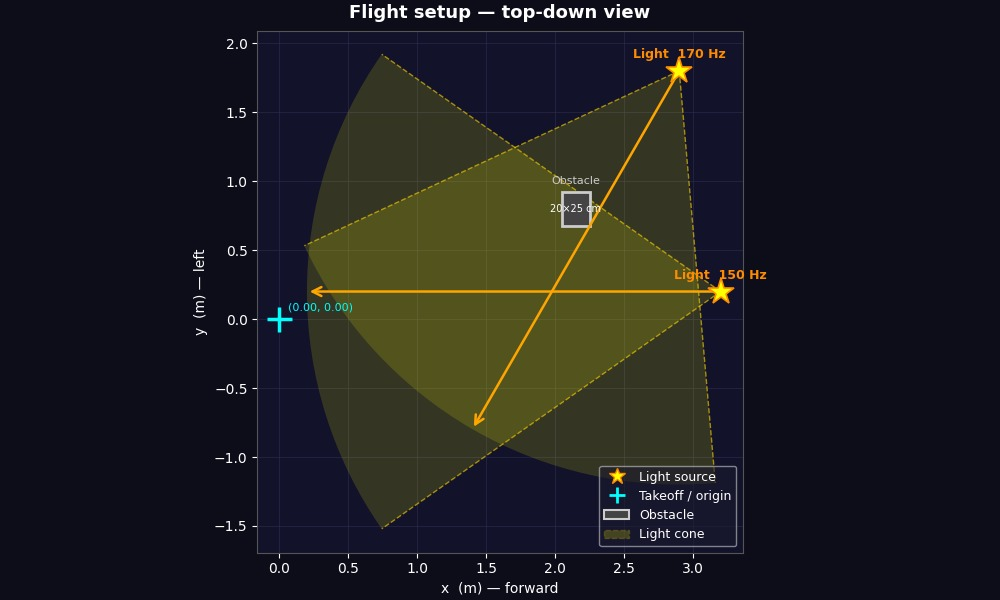
\includegraphics[width=0.6\textwidth]{figures/real_life_setup_plot_with_obstacle.jpeg}
    \caption{Top-down geometry of the real-room obstacle experiment. The room carries the same two beacons as the traverses of Chapter~\ref{chp:multibeacon}; each obstacle flight targets one of them, with the obstacle set into the route toward it and a little to one side. The layout is indicative rather than a precise survey of the room.}
    \label{fig:obstacle-setup}
\end{figure}

\section{SNR Field Mapping}
\label{sec:snr-field}

The fused controller relies on the light map precisely when the beacon is occluded, so before flying the obstacle mission we verify that the real-room SNR field behaves as the design assumes. Two properties must hold: the field must rise toward the beacon, so a gradient exists for the drone to climb, and the obstacle must leave a recognisable mark on it. We check both by surveying the field directly with a dedicated mapping flight, rather than inferring it from a navigation run.

We map the field with a survey flight that covers the area in a regular back-and-forth raster, a lawnmower pattern. The drone holds a fixed altitude of 0.8\,metres, the same height it uses during its navigation flights, so the survey samples the field the controller actually flies through. It moves at a slow, steady speed of about 0.2\,metres per second while logging the SNR at each photodiode, which yields a dense and even coverage of the area. The map records the field in 5\,centimetre cells over an area of about three by one and a half metres, a far denser and more even sampling than any single navigation flight builds. This gives four field maps in all: the two beacons, at 150 and 170\,Hz, each mapped with the obstacle in place and without it.

These maps must be read as a reference, not as a metric survey of the room. Their positions are localised by the drone's own odometry, which drifts over the course of a flight and depends strongly on the drone's starting angle. Even a small initial heading error shifts where the whole surveyed area lands, so the four maps cannot be laid directly on top of one another, and the distances within any one of them are not a true measurement of the room's geometry. What they do show, reliably, is how the SNR field behaves relative to the beacon, and that is all we ask of them. This\todo{What is "this" in this context?} is enough because the controller acts on a heading, not on an absolute beacon position. The algorithm of Chapter~\ref{chp:algorithm} is built around this, so drift in the odometry does not mislead it\todo{Why is this last sentence relevant.}.

Without the obstacle, the SNR field rises smoothly toward the beacon. As Figures~\ref{fig:snr-field-150} and~\ref{fig:snr-field-170} show, each beacon's field climbs from the far side of the room to a clear peak near the beacon, which confirms that the navigable gradient the controller depends on is present in the real room.

Placing the obstacle opens a region of low SNR behind it. Where the box stands between the survey and the beacon, the modulated signal can no longer reach the photodiodes directly, so the recovered SNR drops and leaves a shadow in the field. This shadow is the real-room counterpart of the occlusion the simulation creates with its pillar. It is precisely the region in which the bearing becomes unreliable and the drone must navigate on the stored map instead, the situation the recovering phase of Chapter~\ref{chp:algorithm} is designed to handle. In these survey maps the obstacle is drawn larger than the physical box, whose true size is shown later in the flight plots of Figure~\ref{fig:obstacle-good}. We enlarge it not only in the plots but in the drone's flight code, to leave a margin against odometry drift during the slow raster. The box itself is never bigger. Only the footprint the drone treats as off-limits is enlarged, so it stays clear of the real obstacle.

The 170\,Hz field also appears to carry a slight dip near the 150\,Hz beacon, in a spot where the smooth fall-off alone would lead us to expect a somewhat higher SNR. We read this tentatively as an effect of the 150\,Hz beacon: where that beacon is bright it may begin to saturate the photodiodes, flattening their response and lowering the recovered SNR across all frequencies, the 170\,Hz one included. The dip is faint, and the survey cannot separate it cleanly from the ordinary fall-off with distance, so we note it only as a likely trace of the same close-range saturation that bounds the sensor's operating range, and a reminder that the field is clean only in the band where the photodiodes are neither starved nor saturated.

\begin{figure}[h]
    \centering
    \subfigure[No obstacle]{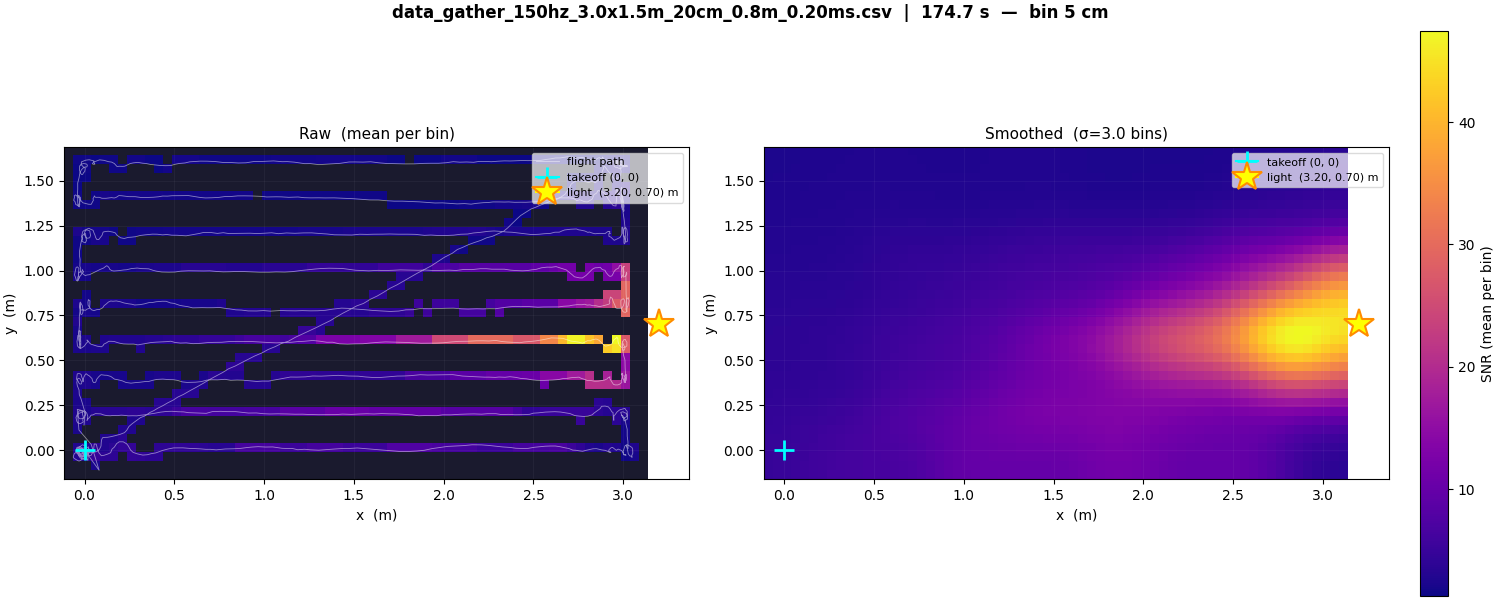
\includegraphics[width=\textwidth]{figures/real_data_gather_flights/150hz_lawnmower_no_obstacle.png}}\\
    \subfigure[With obstacle]{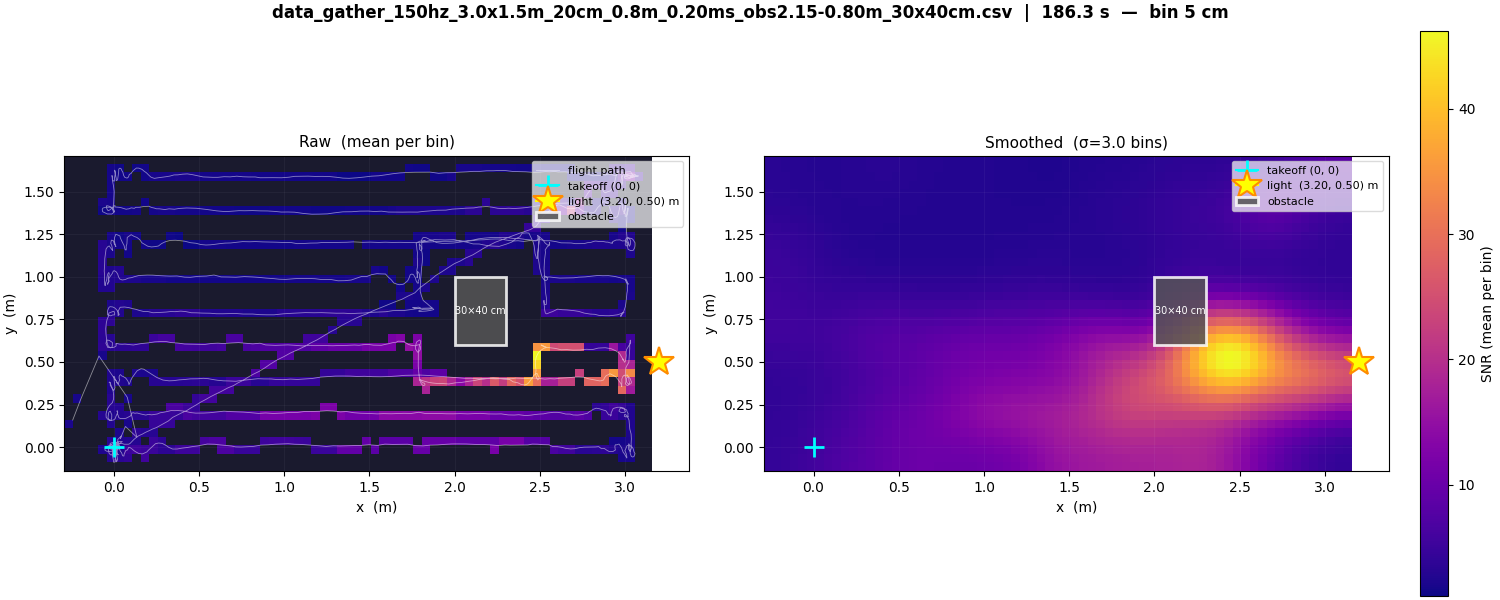
\includegraphics[width=\textwidth]{figures/real_data_gather_flights/150hz_lawnmower_with_obstacle.png}}
    \caption{SNR field of the real room for the 150\,Hz beacon, surveyed on a dense raster at a fixed altitude, without and with the obstacle. Each panel shows the raw per-cell mean alongside a smoothed version, with the flight path overlaid. Without the obstacle the field rises smoothly to a peak at the beacon; with the obstacle a low-SNR shadow opens behind the box. Positions are localised from odometry and serve as a reference, not a metric survey.}
    \label{fig:snr-field-150}
\end{figure}\todo{A small title above the figure showing that its the 150Hz figure would be nice. Also make sure to use separate labels for the subplots. Then also reference the subplots in the text. We should also more explicitly note that the SNR color grade goes from-to different numbers.}

\begin{figure}[h]
    \centering
    \subfigure[No obstacle]{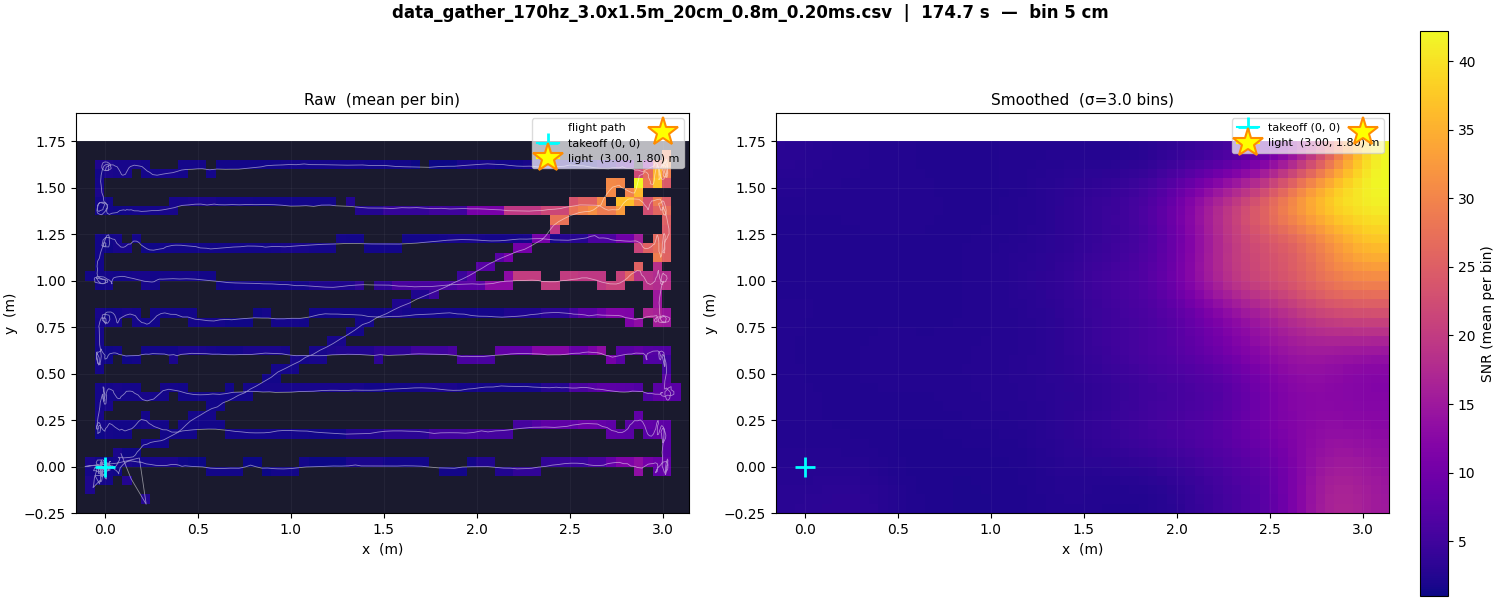
\includegraphics[width=\textwidth]{figures/real_data_gather_flights/170hz_lawnmower_no_obstacle.png}}\\
    \subfigure[With obstacle]{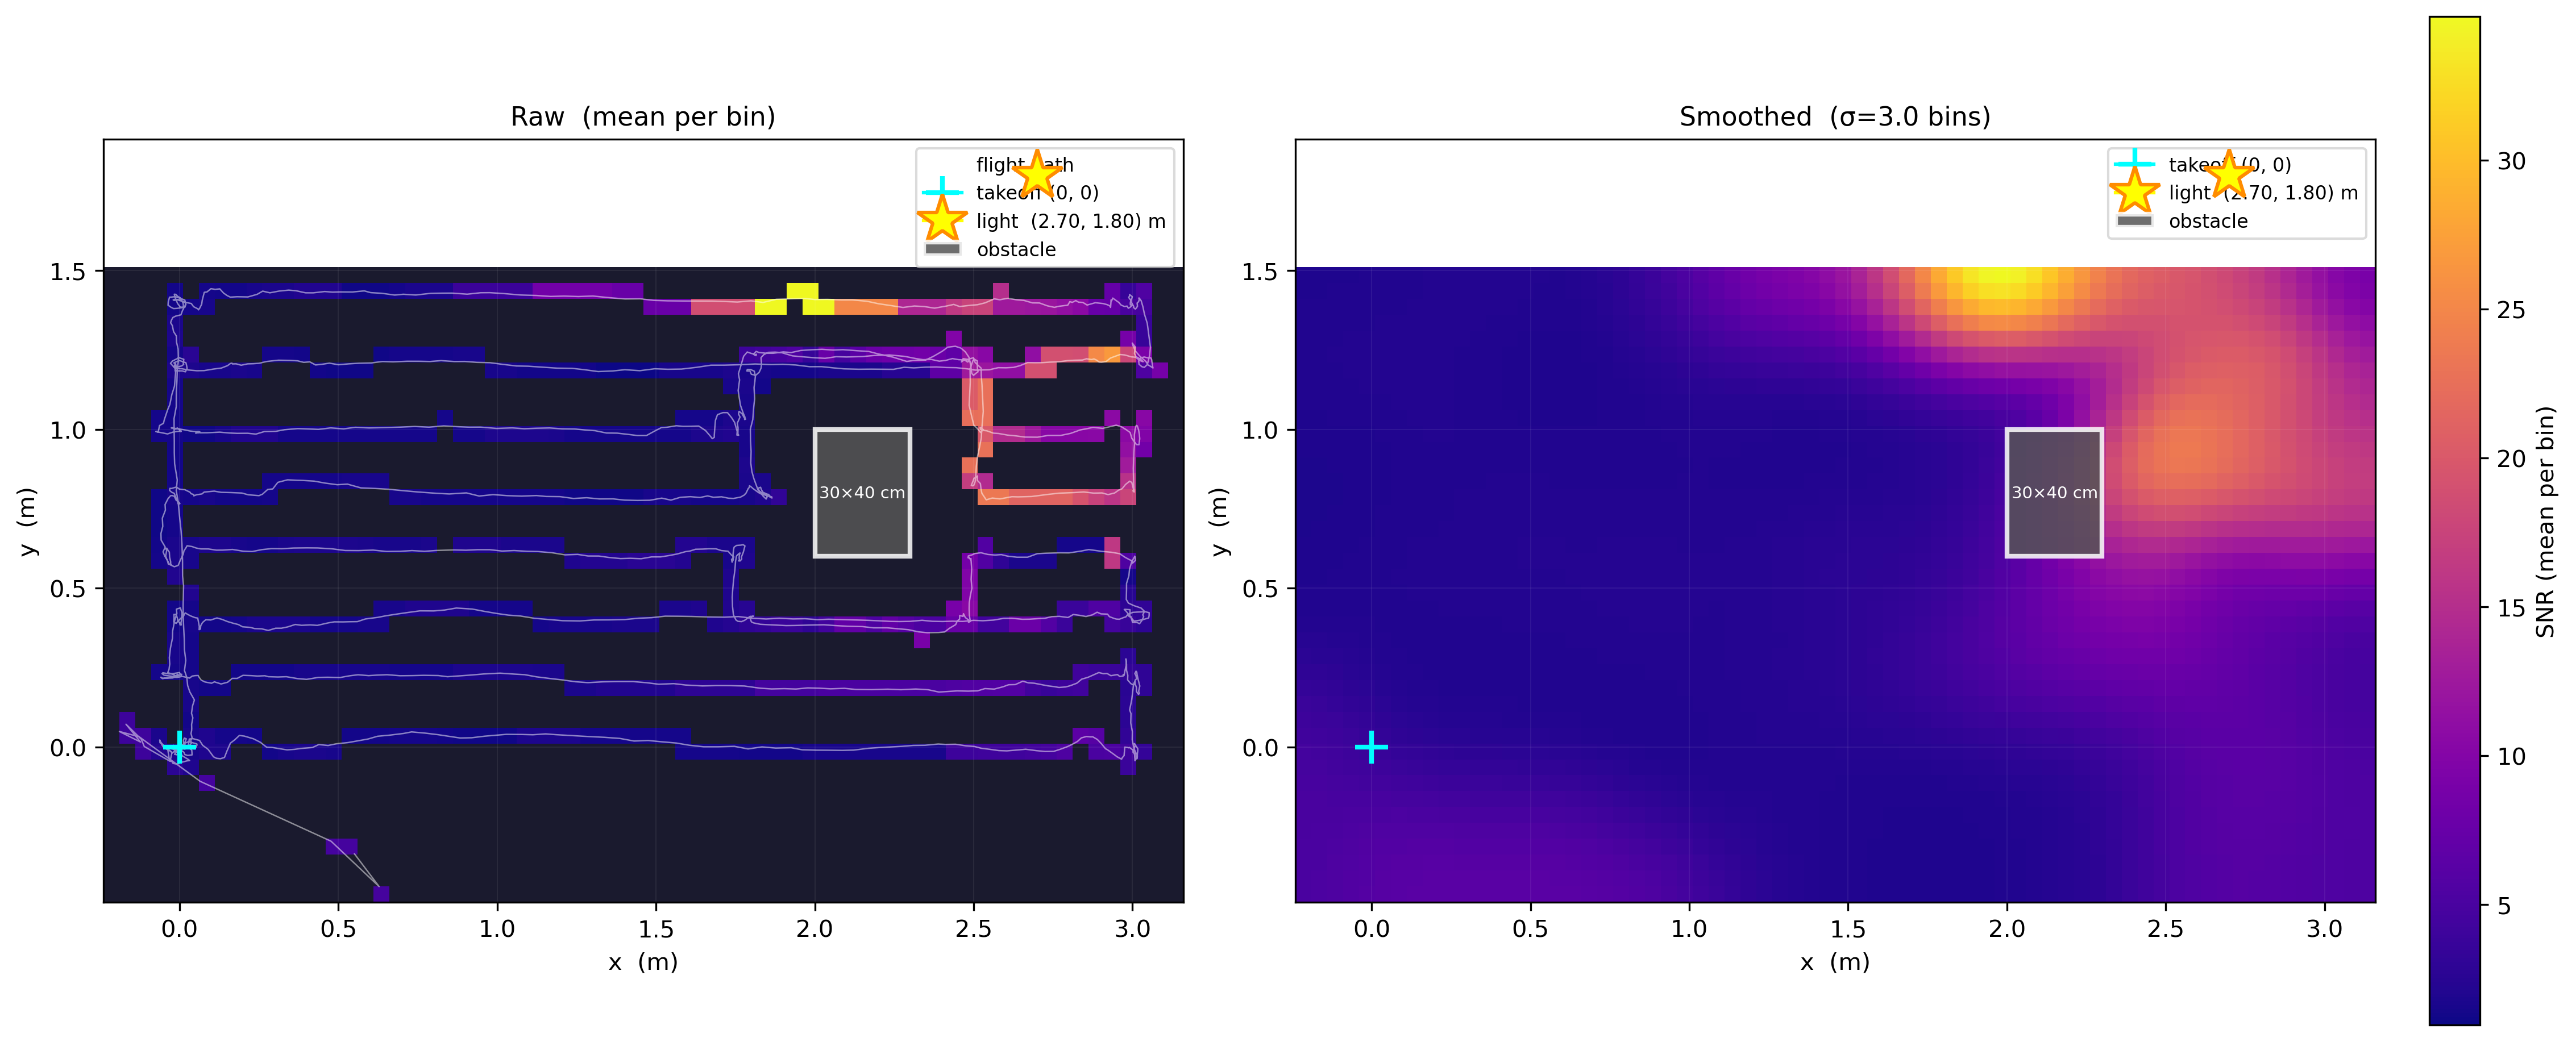
\includegraphics[width=\textwidth]{figures/real_data_gather_flights/170hz_lawnmower_with_obstacle.png}}
    \caption{SNR field of the real room for the 170\,Hz beacon, without and with the obstacle, in the same format as Figure~\ref{fig:snr-field-150}. The field again rises to a peak near the beacon and shows the obstacle's shadow. A slight dip also appears near the 150\,Hz beacon, which we tentatively attribute to that beacon saturating the photodiodes and lowering the recovered SNR across all frequencies.}
    \label{fig:snr-field-170}
\end{figure}

\section{Obstacle Avoidance}

\subsection{Simulation}

With the SNR field confirmed navigable, we turn to the avoidance task itself. In simulation the fused controller solves the task that defeated both baselines of Chapter~\ref{chp:algorithm}. Flying the same scene, from the same start toward the same beacon as the bearing-only and gradient-only runs, it routes cleanly around the obstacle and reaches the beacon, as Figure~\ref{fig:fused-sim} shows. After a brief opening segment on the bearing alone, while the map is still too sparse for a reliable gradient, the controller blends in the gradient and from then on steers by the combined bearing-and-gradient heading\todo{This sentence is overly long and should be split.}. This blended heading curves the path around the pillar on its own, so the drone neither flies into the obstacle nor has to stop and search. The avoidance here comes from the fusion of the two cues rather than from the recovering fallback, which this run never needs to enter, since the bearing remains valid throughout the curved approach. This contrast with the baselines \todo{Which baselines?} is the central result of the run: the bearing-only controller collides with the pillar in Figure~\ref{fig:bearing-fail} and the gradient-only controller stalls in Figure~\ref{fig:gradient-fail}, whereas the fused controller\todo{Is this not too much duplicate information?}, holding both the immediate bearing and a memory of the field, rounds the obstacle and arrives.

\begin{figure}[h]
    \centering
    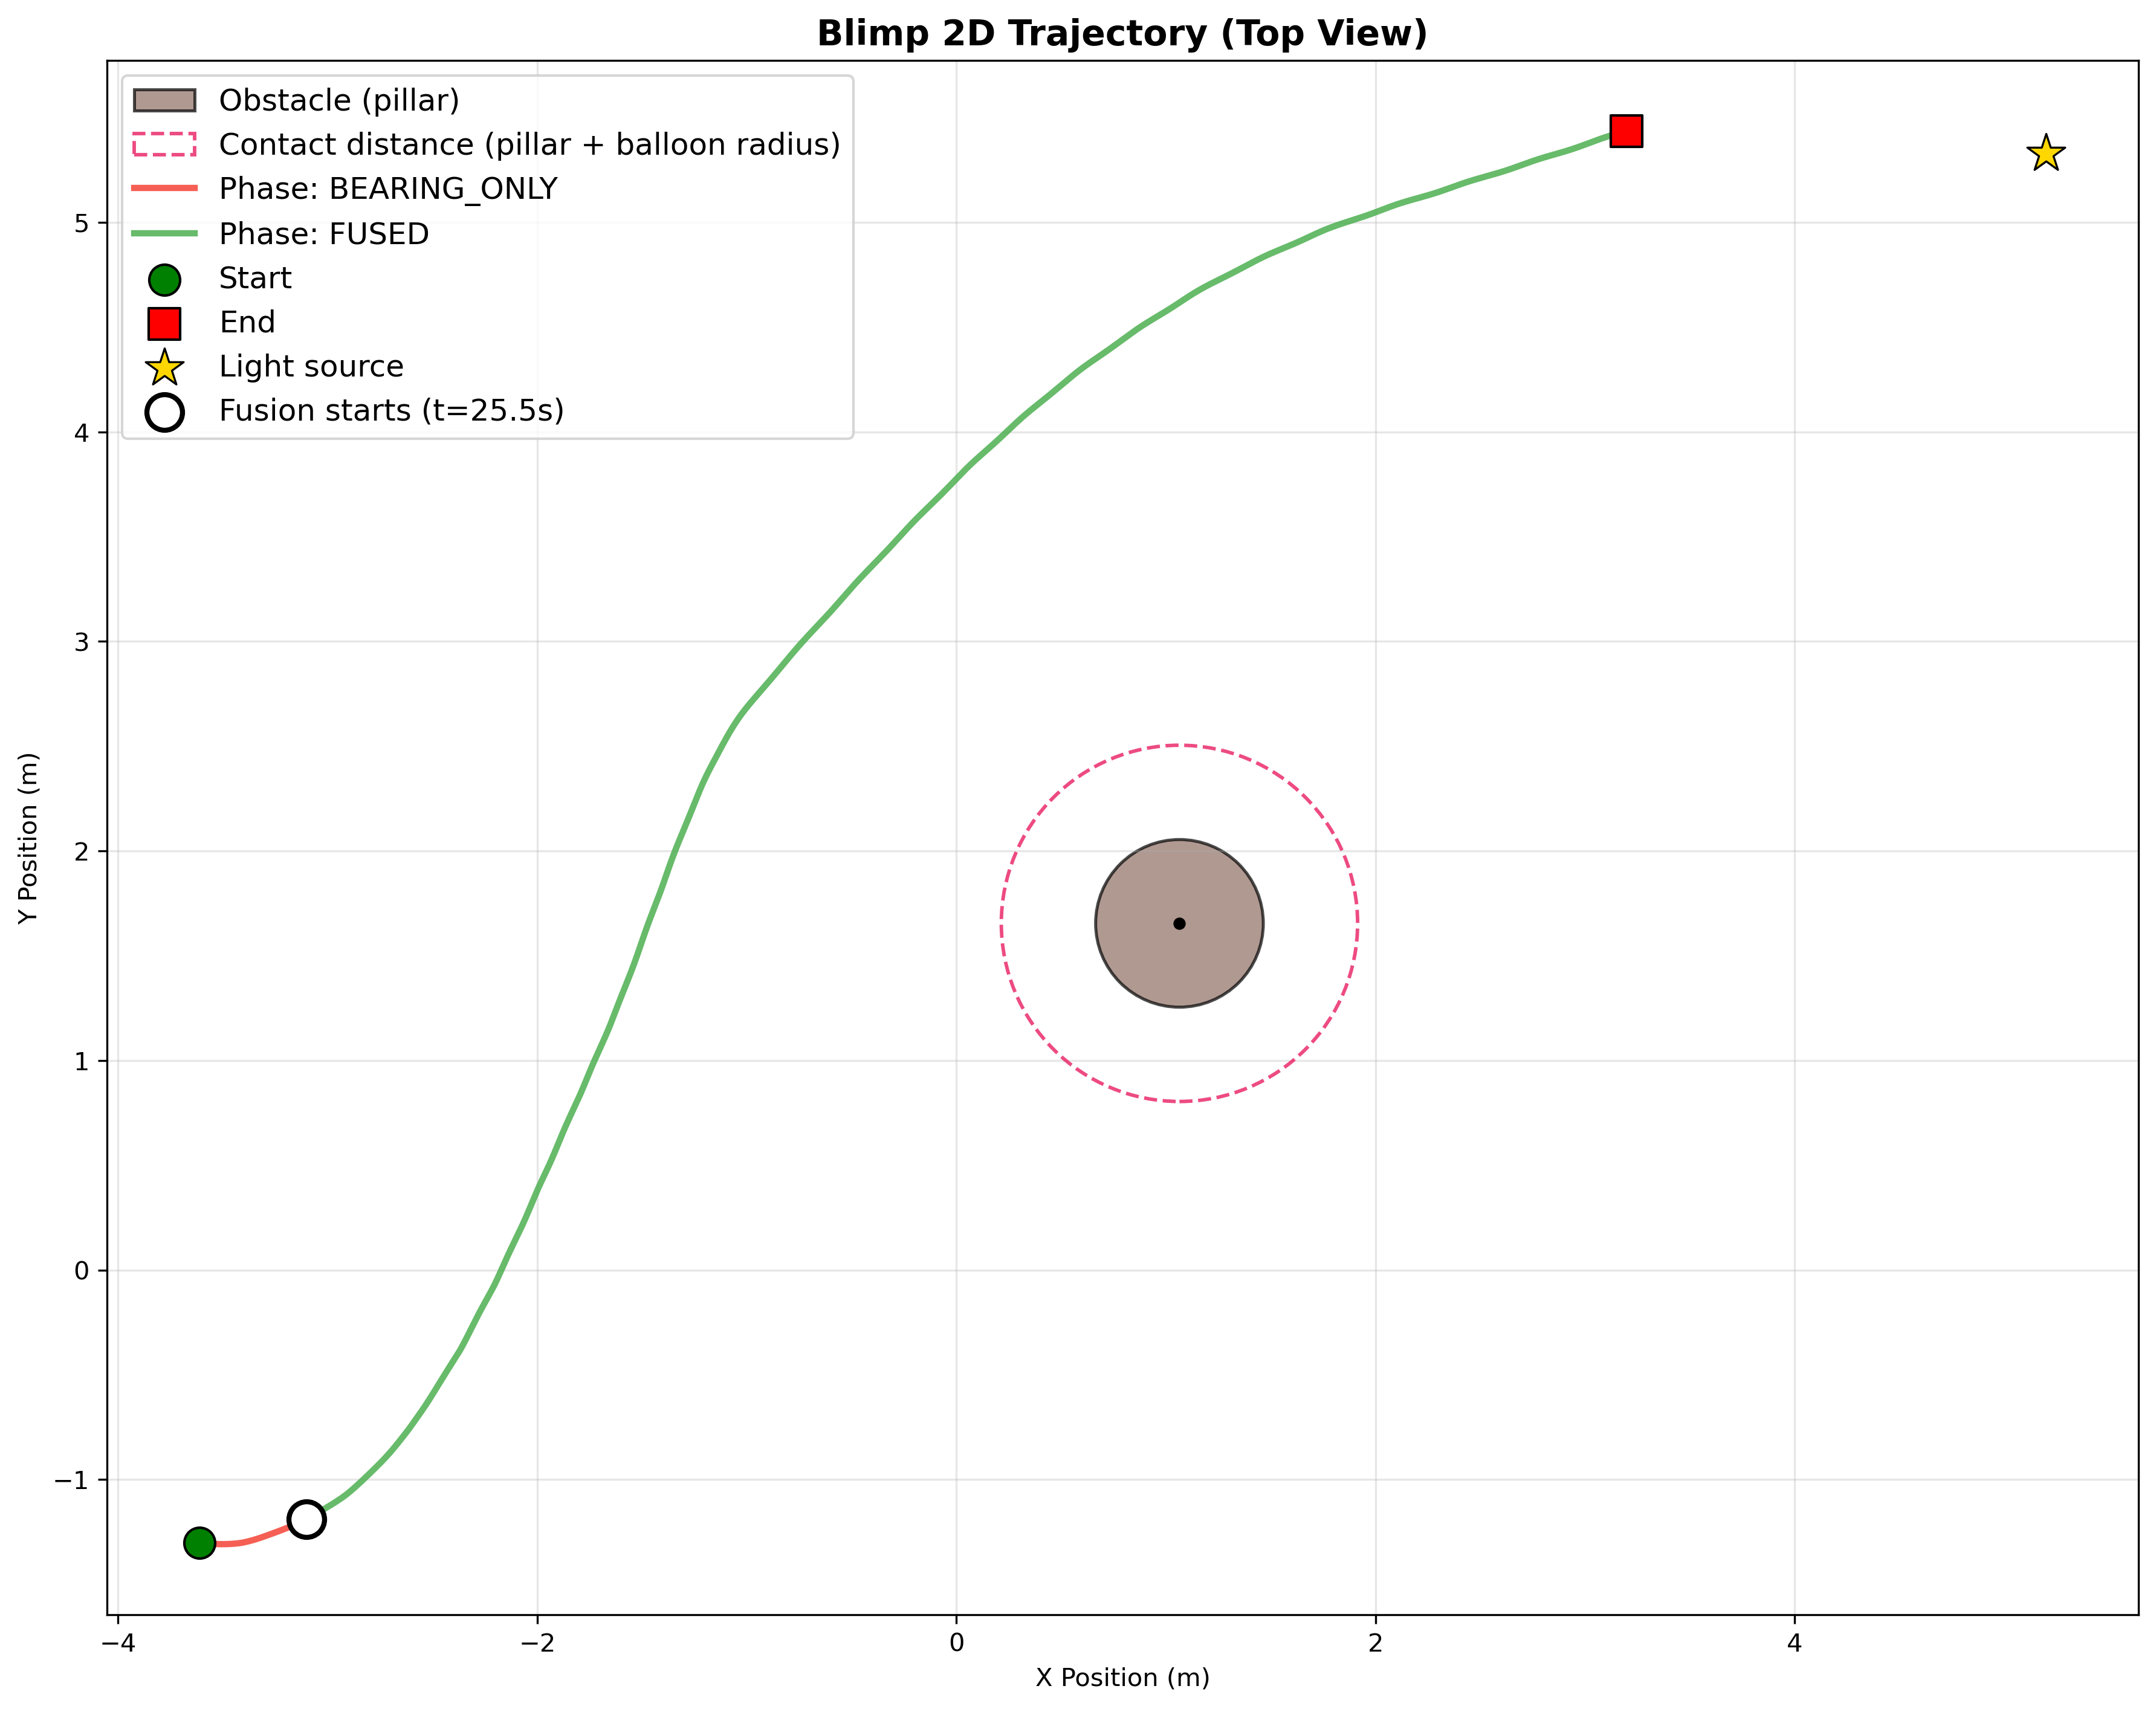
\includegraphics[width=0.6\textwidth]{figures/fused_sim/blimp_trajectory_2d.png}
    \caption{In simulation, the fused controller routes around the obstacle and reaches the beacon on the blended bearing-and-gradient heading, where the bearing-only and gradient-only controllers fail in Figures~\ref{fig:bearing-fail} and~\ref{fig:gradient-fail}.}
    \label{fig:fused-sim}
\end{figure}

\subsection{Real-World Flight}

Simulation removes the ambient light and motor noise of real flight, so we now fly the obstacle mission on the CrazyFlie to confirm the behaviour survives them\todo{Too coloquial and informal.}. The drone takes off from its origin and heads for a single beacon, with the box set into the route a little to one side of the straight-line path.

We present two runs that bring the drone close to the obstacle. We fly the mission several times, and the drone reaches the beacon on every run, but on many of them the path stays clear of the box, so the obstacle never comes into play. The two we show pass close to it, where the controller must contend with the obstacle, and they exercise it in two different ways.

In both flights the drone reaches the beacon, steering around the box rather than into it, and the controller registers its arrival and dwells. We do not run a controlled repeatability trial, so these results demonstrate that the avoidance works rather than measuring how reliably it succeeds.

In the first flight the beacon signal weakens enough that the controller falls back on the map, exercising the recovering phase that the simulation never needed. Figure~\ref{fig:obstacle-good} shows the result. The upper panel plots the path leaving the origin and steering past the box, drawn over the light map the drone builds as it flies, whose cells are coloured by the SNR measured there. The lower panel tracks the controller's state and the overall SNR over time. The flight walks the state machine of Chapter~\ref{chp:algorithm} through searching, aligning, and approaching, and then, as the drone passes behind the obstacle, into recovering and back. As it moves behind the box the beacon is occluded, the overall SNR falls to a trough\todo{Colloquial -- and this sentence is a bit long. Maybe split.}, and the magnitude of the bearing estimate drops below its trust threshold, so the bearing no longer yields a usable heading. This is exactly the situation a purely reactive controller cannot handle: with no memory of the field it would have no direction left to follow. The stored map supplies one. Because the gradient fitted to the map still meets its reliability conditions, the state machine enters recovering and the drone continues on the gradient direction alone, climbing the stored field to move out of the obstacle's shadow. As soon as the bearing rises back above its trust threshold the controller returns to approaching, closes on the beacon, and dwells.

\begin{figure}[h]
    \centering
    \subfigure[Flight path over the light map the drone built]{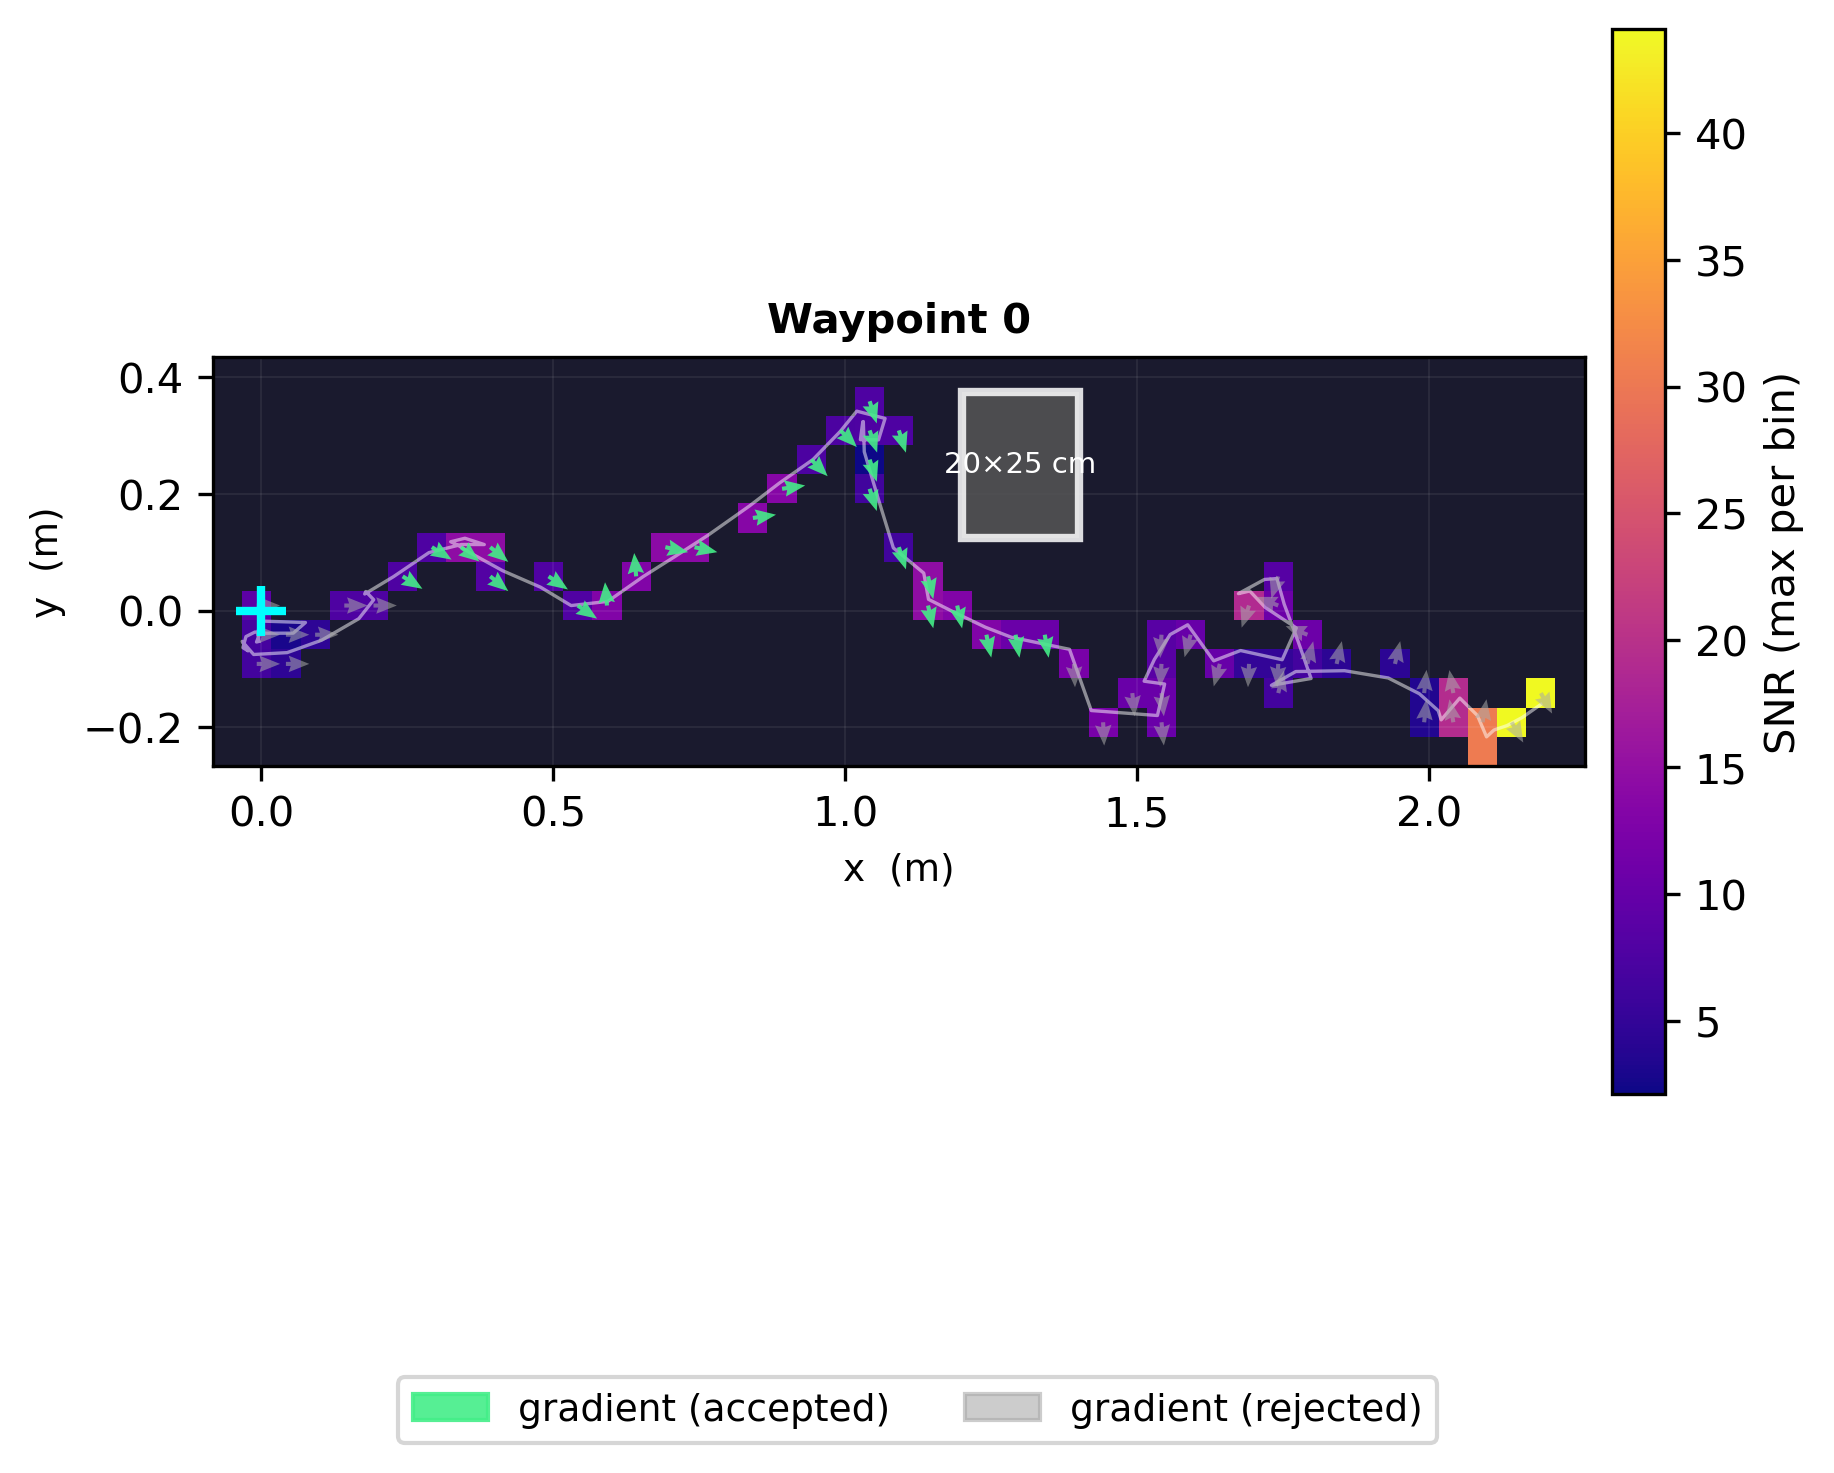
\includegraphics[width=0.85\textwidth]{figures/obstacle_dodging_real/one_waypoint_good_dodge_trajectory.png}}\\
    \subfigure[Controller state and overall SNR over time]{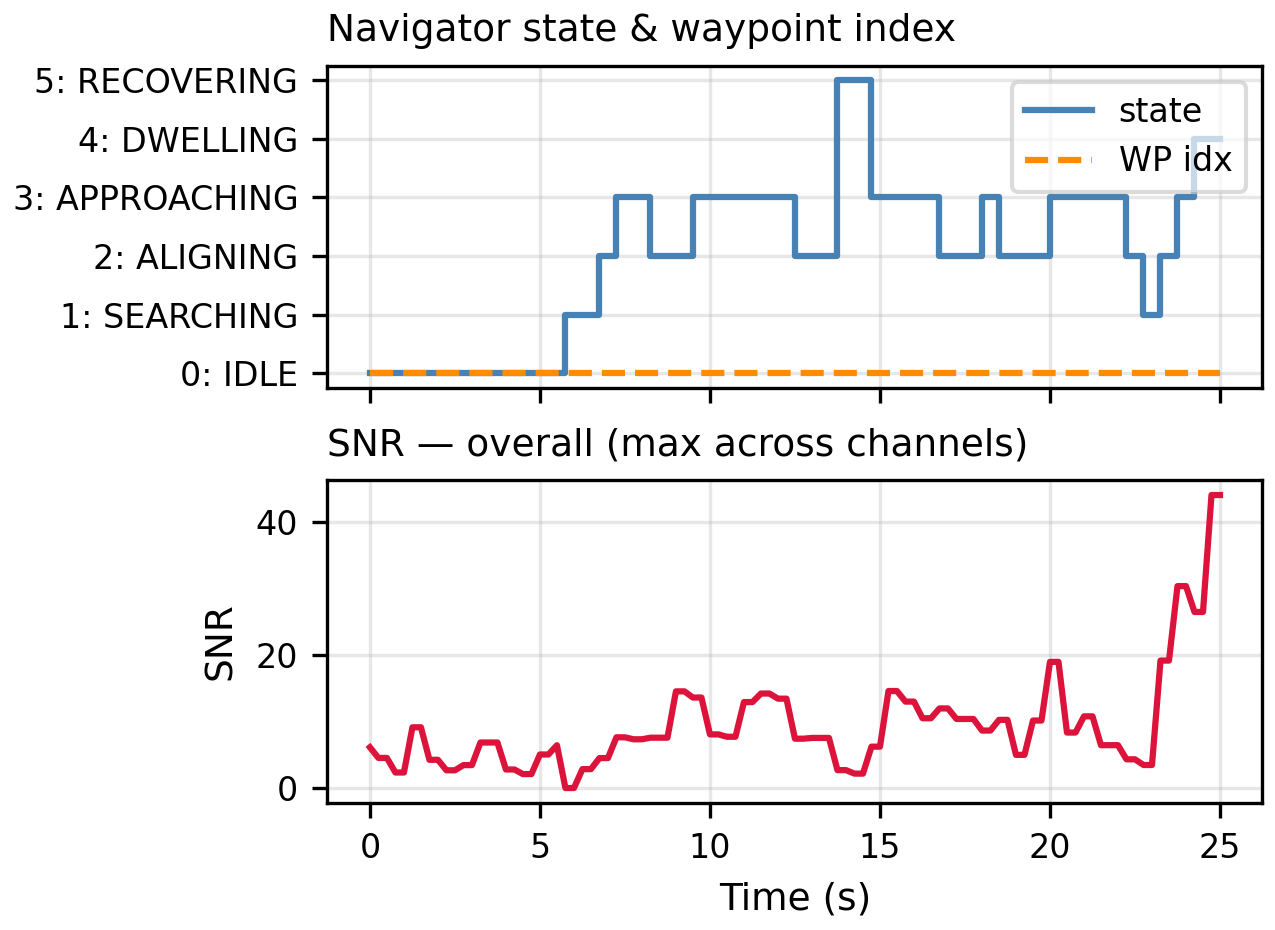
\includegraphics[width=0.85\textwidth]{figures/obstacle_dodging_real/one_waypoint_good_dodge_state_snr.png}}
    \caption{Real-world obstacle flight on the CrazyFlie~2.1. The drone steers around the box to reach the beacon; as it rounds the obstacle the SNR falls and the bearing becomes unreliable, so the state machine enters the recovering phase and follows the gradient map alone until the signal comes back.}
    \label{fig:obstacle-good}
\end{figure}

The second flight reaches the beacon without ever falling back on the map alone, and so represents the other operating regime. The difference between the two flights is geometric rather than a change in the controller: the first passes through more of the box's shadow, where the beacon is occluded and the bearing is lost, whereas the second skirts the shadow's edge. The drone therefore keeps a usable bearing throughout, so the controller stays in its approaching phase and never enters recovering. The blended bearing-and-gradient heading alone is enough to steer the path around the obstacle, as Figure~\ref{fig:obstacle-dodge} shows. Taken together, the two flights show the controller drawing on the map only as far as each situation requires: recovering on the gradient when the bearing drops below its trust threshold, and rounding the obstacle on the fused heading when it does not.

\begin{figure}[h]
    \centering
    \subfigure[Flight path over the light map the drone built]{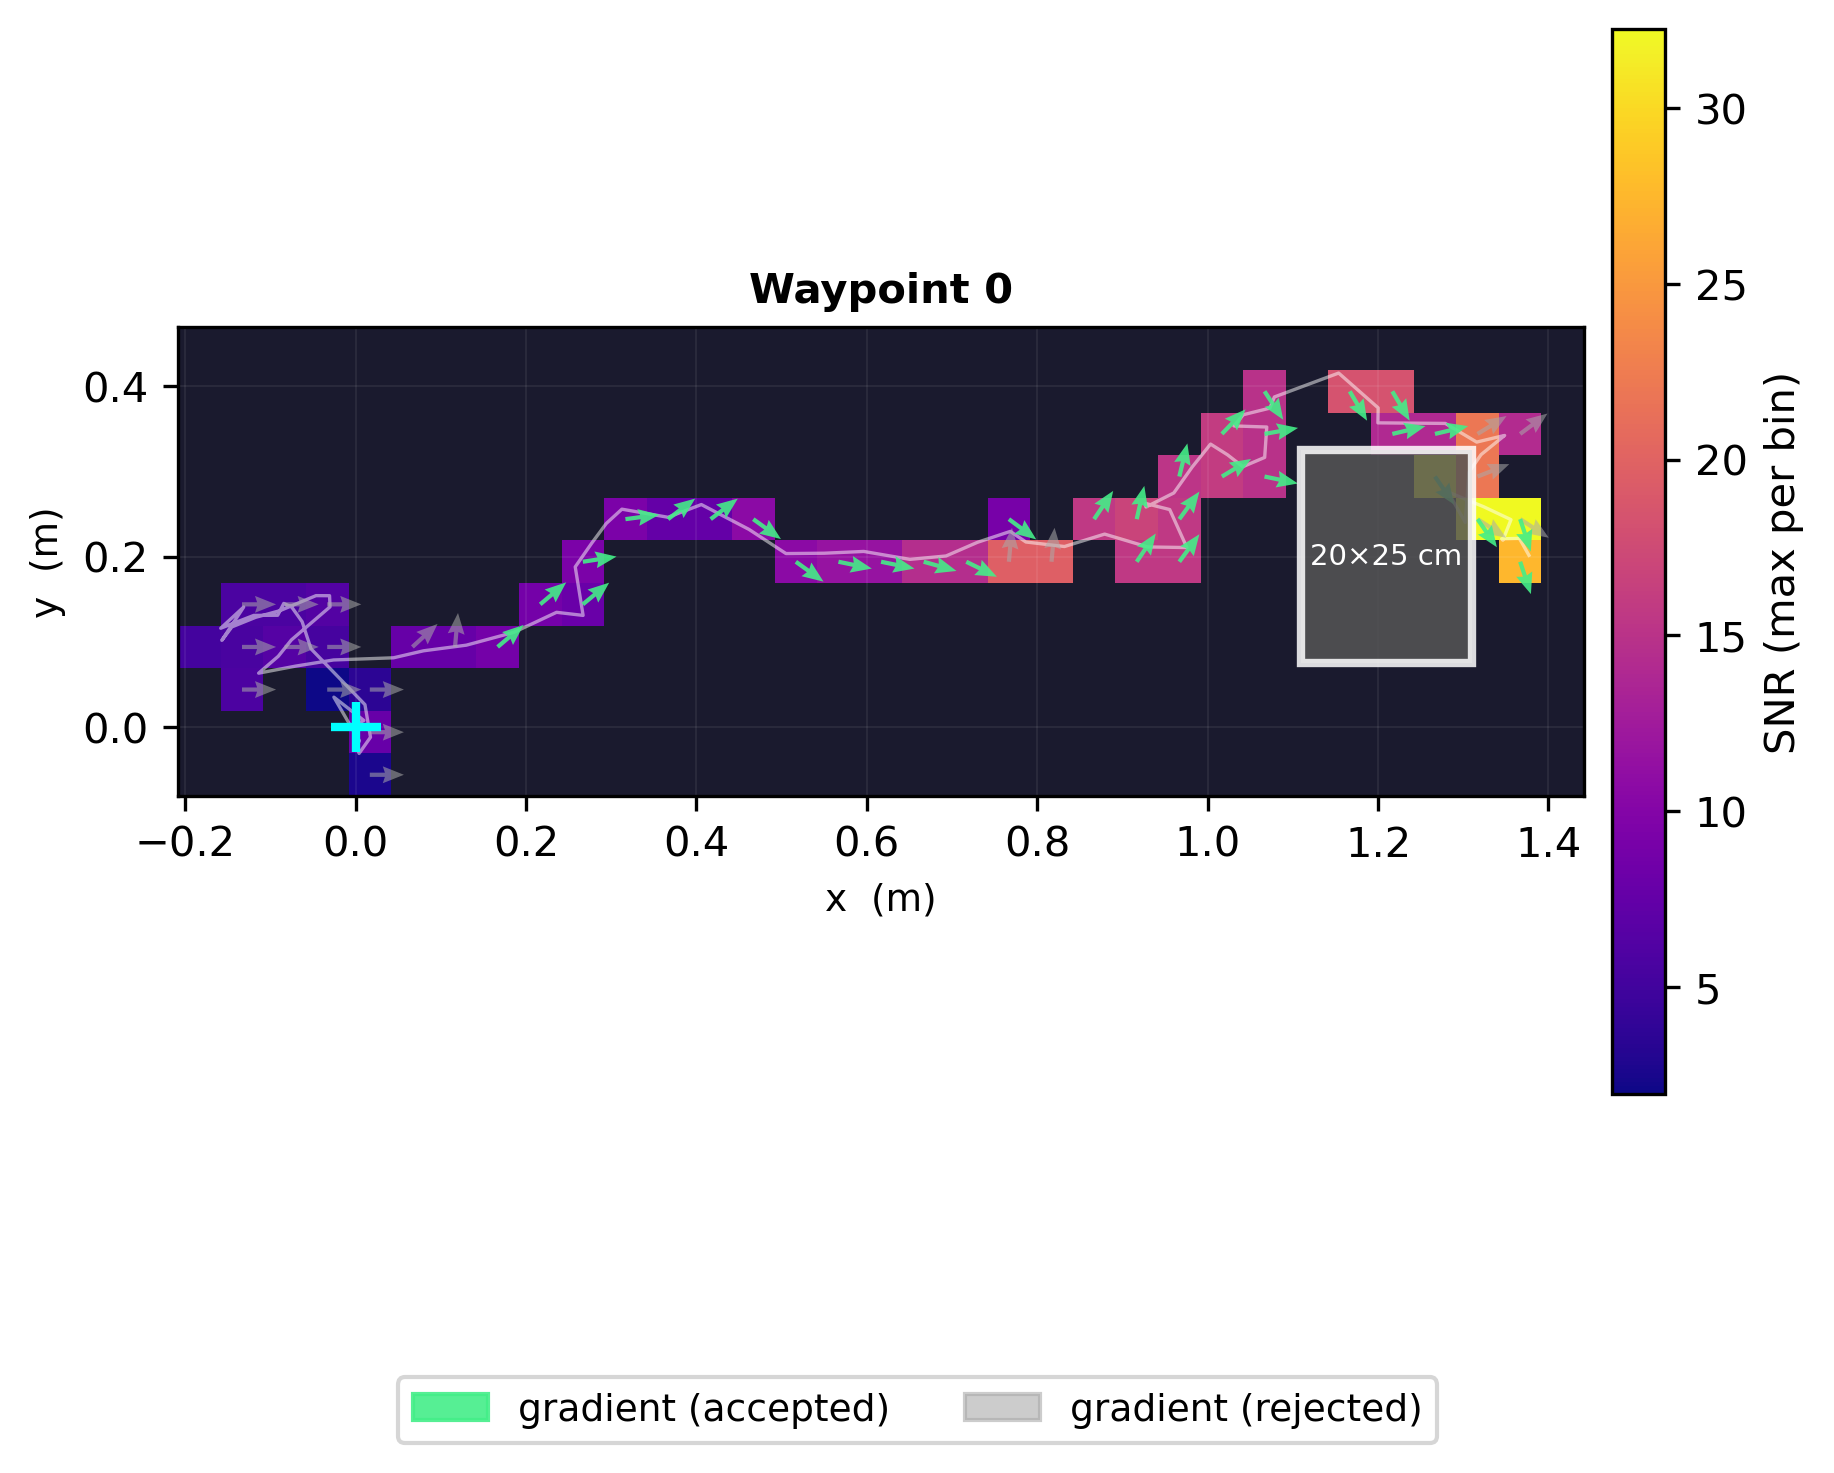
\includegraphics[width=0.85\textwidth]{figures/obstacle_dodging_real/one_waypoint_dodges_obstacle_trajectory.png}}\\
    \subfigure[Controller state and overall SNR over time]{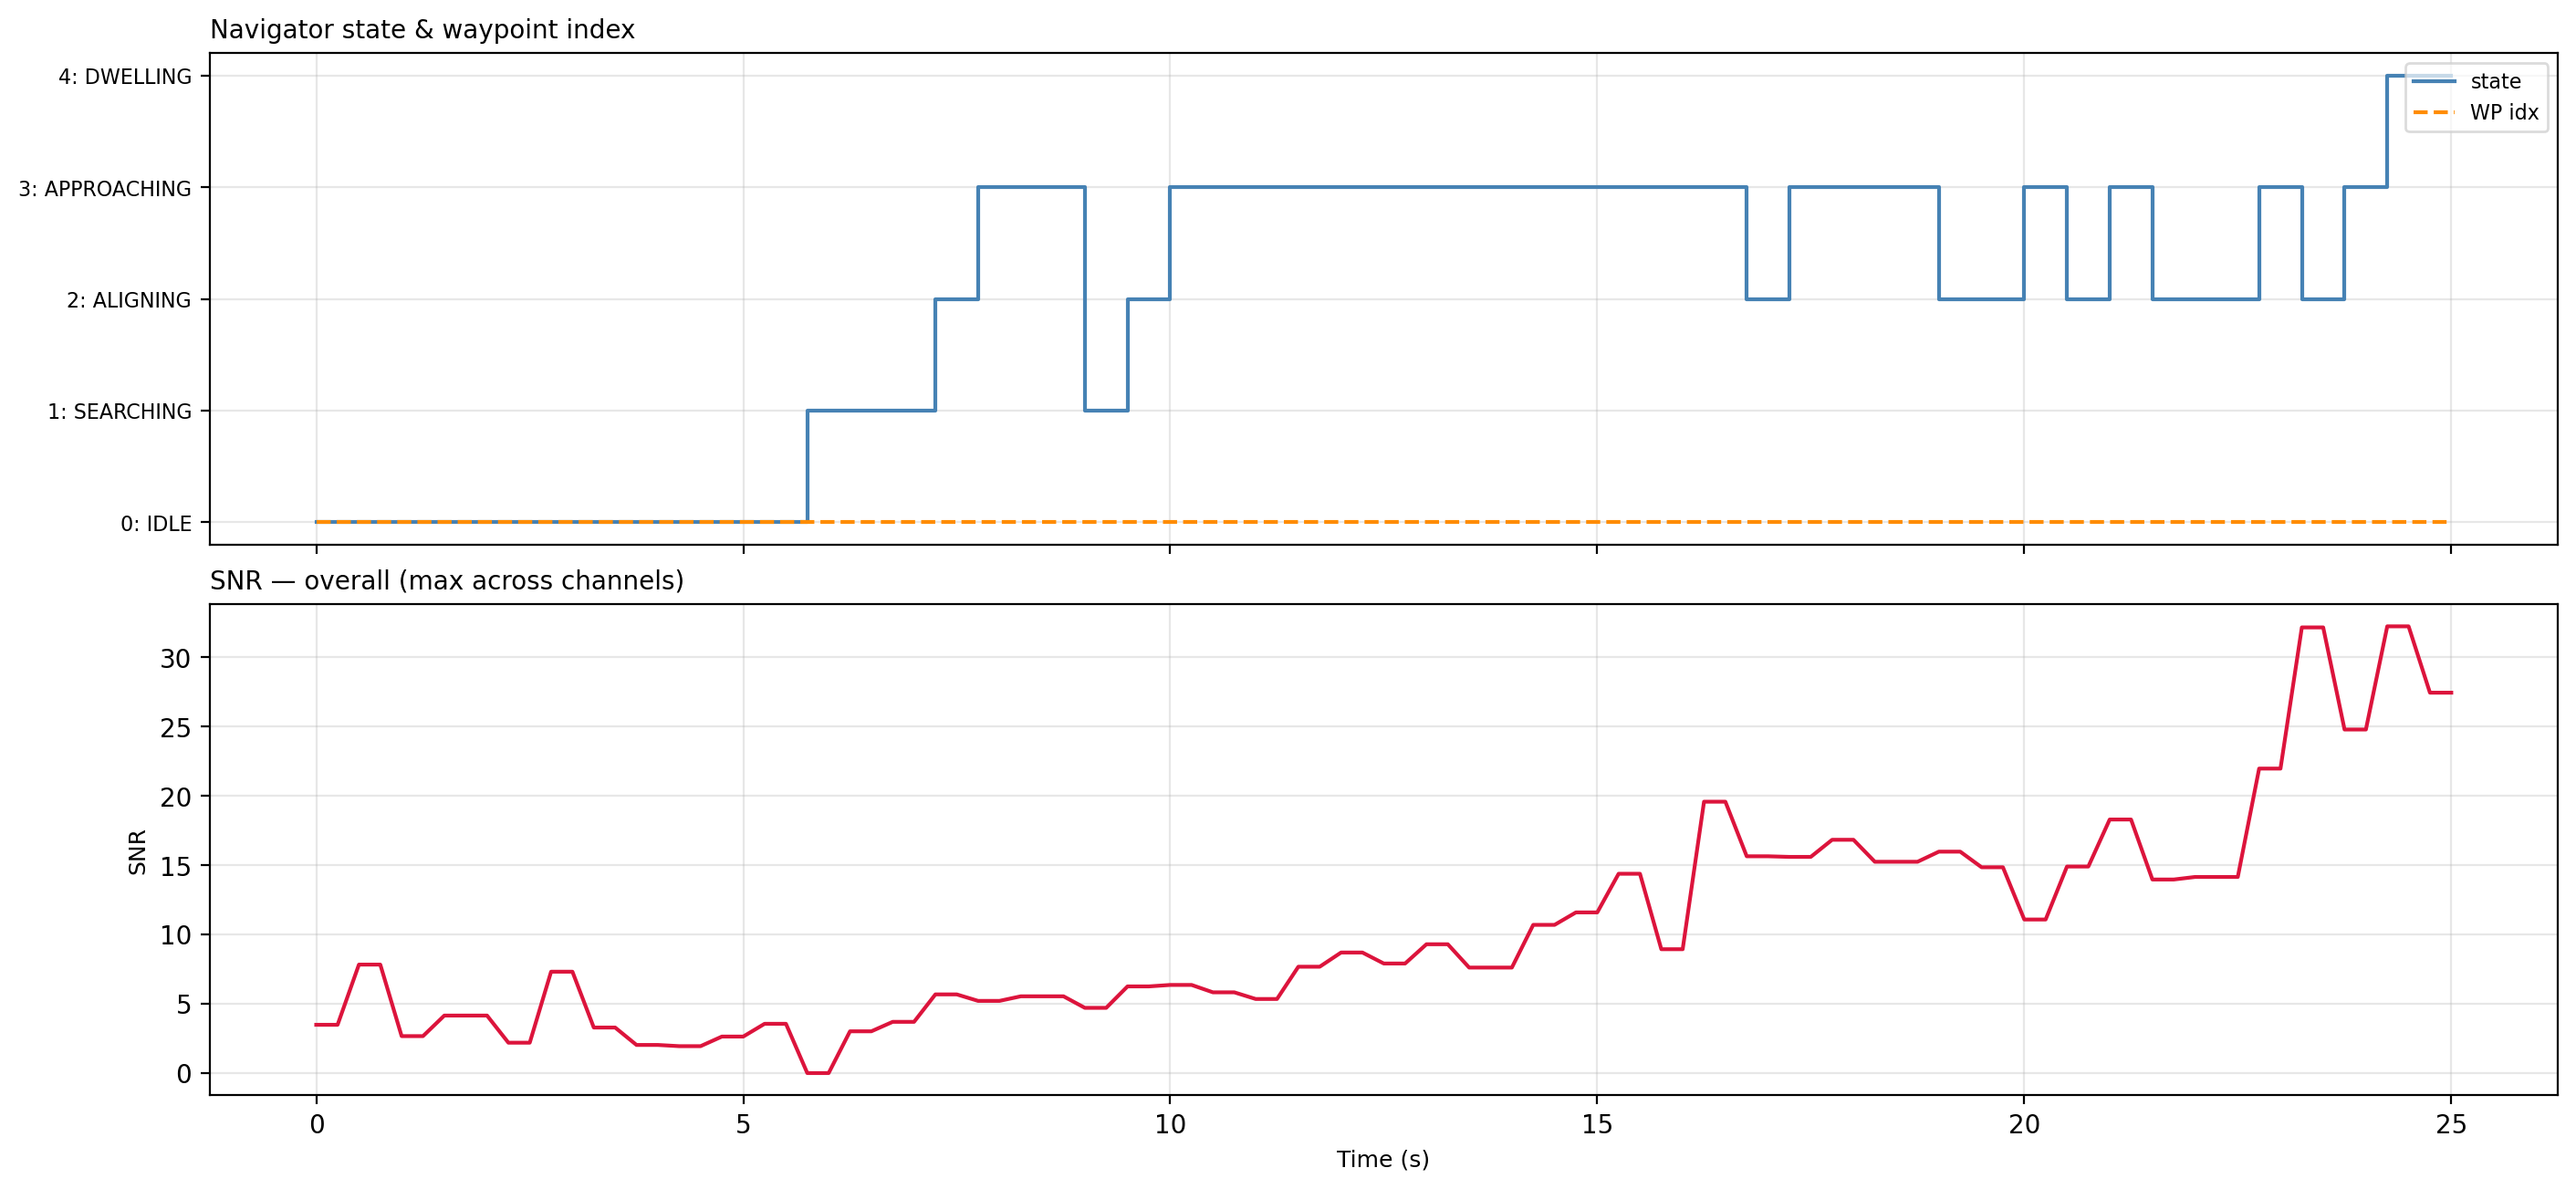
\includegraphics[width=0.85\textwidth]{figures/obstacle_dodging_real/one_waypoint_dodges_obstacle_state_snr.png}}
    \caption{A second real-world obstacle flight in which the drone keeps a usable bearing throughout, so the controller stays in its approaching phase and steers around the box on the blended heading without ever entering the recovering phase.}
    \label{fig:obstacle-dodge}
\end{figure}

\section{Generalisation to a Blimp Platform}

Our own validation spans the Webots simulation and the CrazyFlie~2.1, but the contribution is not tied to that platform. We show this through a collaboration with Huang et al.~\cite{huang2026lta}, who developed the lighter-than-air blimp and the Webots simulation this thesis builds on. The blimp is a closely related micro-drone, held aloft by a helium balloon and driven by a different motor layout. The base bearing and single-photodiode gradient methods of Huang et al. were demonstrated on this blimp only in simulation, never flown on the real airframe~\cite{huang2026lta}. The real blimp flights instead use the contribution of this thesis. We develop the fused controller within the simulation, build the photodiode board of Chapter~\ref{chp:hardware}, and run the real-world experiments of this thesis on the CrazyFlie \todo{Why is this sentence here? Feels superfuous.}. Huang et al. then mounts the same board and fused controller on the real blimp, adapting only the low-level control to its motor layout, and confirms that it reaches several modulated beacons in turn and avoids obstacles there \todo{What is this "there"}, as it does on the CrazyFlie~\cite{huang2026lta}. The same board and algorithm therefore work across two different airframes, which shows that the approach depends on the light sensing rather than on the specifics of the platform.

The blimp flights also show a higher SNR than we obtain on the CrazyFlie. The photodiode board is the same and sits in the same place on both airframes, since the blimp is in essence\todo{colloquial.} a CrazyFlie with a different motor layout and a helium balloon on top. What differs is the motors: a buoyant platform stays aloft without constantly driving the motors, so on the blimp they run only when it moves and at far lower power.

\subsection{Motor Noise on the CrazyFlie}

The higher SNR on the blimp points to the motors as the likely cause, so we measure their effect directly on the CrazyFlie. We hold the board at a fixed pose and record the SNR while running an increasing number of its motors, both with the hardware anti-alias filter and without. Table~\ref{tab:motor-noise} and Figure~\ref{fig:motor-noise} show the result. The SNR falls steadily as more motors spin. With the hardware filter in place it drops from about 61 with all motors off to about 25 at full throttle, which confirms the motors are the dominant disturbance.

A motor couples noise into the board in two ways: it draws current that interferes electrically, and it shakes the board mechanically. To separate the two, we repeat the four-motor case with the motors moved onto extension wires, which isolates them mechanically while leaving them electrically connected. With the filter in place this recovers about half of the lost SNR, from about 25 back to about 43. Vibration and electrical interference therefore contribute in roughly equal measure, once the filter has dealt with the worst of the aliased noise.

The motors are therefore the main reason the CrazyFlie sees a lower SNR than the blimp. Because the blimp drives its motors far less, it avoids most of this penalty\todo{What penalty?}, which explains its higher SNR and the longer sensing range that comes with it\todo{Where does this longer sensing range come from? Did we already explain the relation to higher SNR and more range in a different chapter? Otherwise maybe leave it out.}. What this extra range could buy, and how a future board might suppress the mechanical half of the loss, we take up in Chapter~\ref{chp:futurework}.\todo{The future work forward reference is maybe not needed.}

\begin{table}[ht]
    \centering
    \caption{Overall SNR on the CrazyFlie at a fixed pose while running an increasing number of its motors, with the hardware anti-alias filter left unpopulated and with it soldered. Each cell is the mean $\pm$ standard deviation. The last row repeats the four-motor case with the motors moved onto extension wires, mechanically isolating them from the board.}
    \label{tab:motor-noise}
    \begin{tabular}{l c c}
        \hline
        Configuration & No HW filter & HW filter \\
        \hline
        0 motors                & $26.7 \pm 1.8$  & $60.6 \pm 16.3$ \\
        1 motor                 & $24.2 \pm 1.8$  & $49.2 \pm 10.9$ \\
        2 motors                & $23.2 \pm 1.7$  & $46.0 \pm 9.0$  \\
        3 motors                & $18.0 \pm 2.3$  & $28.7 \pm 3.2$  \\
        4 motors                & $16.7 \pm 2.2$  & $24.8 \pm 2.6$  \\
        \hline
        4 motors, extension wires & $19.3 \pm 1.5$ & $43.1 \pm 7.3$ \\
        \hline
    \end{tabular}
\end{table}

\begin{figure}[ht]
    \centering
    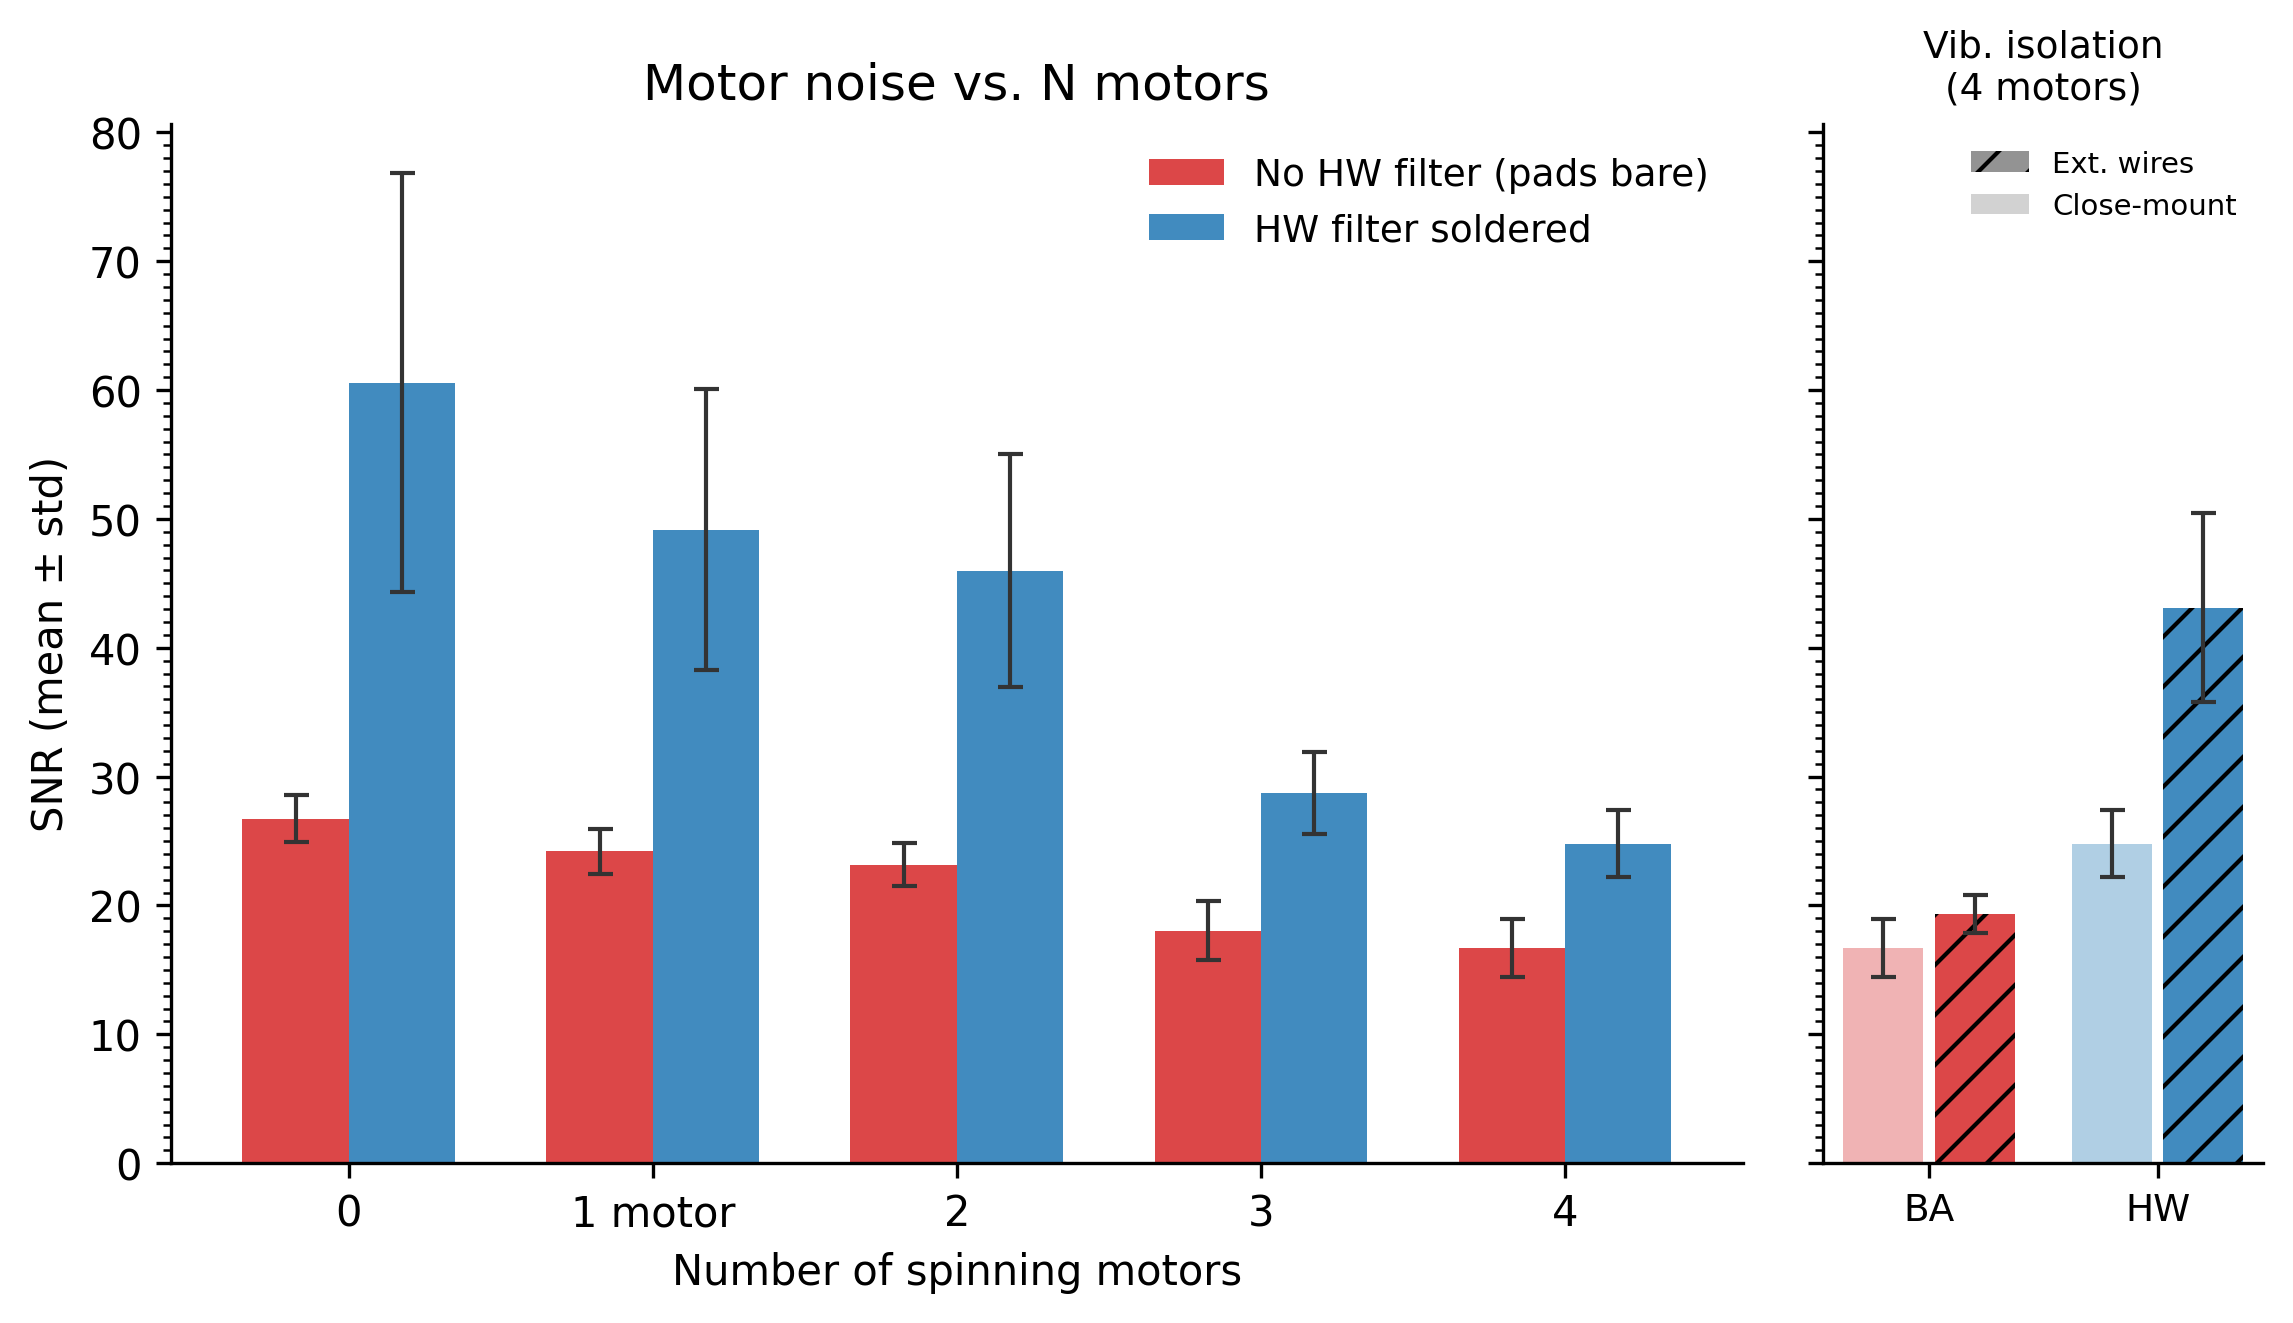
\includegraphics[width=0.85\textwidth]{figures/motor_noise.png}
    \caption{Overall SNR on the CrazyFlie as the number of running motors increases, with the hardware anti-alias filter unpopulated and soldered. The SNR falls as more motors spin, and the rightmost configuration moves the four motors onto extension wires to isolate their vibration from the board.}
    \label{fig:motor-noise}
\end{figure}\todo{The figure now contains BA and HW and are not explained. Please put explaination in the caption. }

This result\todo{What result?} connects back to the motivation of Chapter~\ref{chp:introduction}. The prior work we set out to extend could reach only a single beacon in open space, whereas the board and fused controller developed here now give that same platform the multi-beacon, obstacle-aware navigation it lacked.\todo{This paragraph feels misplaced. Almost as if it should be in the conclusion.}


% Create conclusions
\chapter{Conclusions and Future Work}
\label{chp:conclusions}

In this thesis, we ask a central question for autonomous drone deployment: how can autonomous navigation be provided on a weight-, size-, and power-constrained micro-drone with minimal changes to the environment? We address this question with a visible-light navigation system that uses lightweight on-board light sensing to guide the drone toward modulated light beacons, requiring only minimal modification to existing lighting infrastructure. To make the system robust in cluttered indoor environments, we extend it so the drone can visit several beacons in succession and reach a beacon whose direct light an obstacle partly blocks.

The work builds on the light-guided navigation system proposed by Huang et al.~\cite{huang2026lta}, especially their bearing-angle estimation and gradient-based light-source seeking algorithms. The bearing estimate provides an immediate direction toward a visible beacon, but it keeps no memory of the space the drone has already observed. The gradient method, in contrast, can follow changes in the light field, but it is slower because it must infer direction from measurements gathered during motion. These methods are insufficient for the more realistic missions considered in this thesis. They do not by themselves provide robust sequencing across multiple beacons. A bearing-only controller can also fail when an obstacle weakens or blocks the direct light signal, even though the bearing is the most efficient method in open-space source seeking.

This thesis set out to overcome these limitations within the constraints of a micro-drone. Meeting its two goals required solving four challenges, which follow from the three research questions of Chapter~\ref{chp:introduction}. Table~\ref{tab:rq-mapping} maps the research questions onto these challenges and goals. The following paragraphs discuss each challenge and how this thesis addresses it.

\begin{table}[htbp]
    \centering
    \caption{How the three research questions of Chapter~\ref{chp:introduction} map onto the four challenges solved in this thesis and the two navigation goals they enable. The first research question concerns feasibility and underpins both goals; the second and third are the goals themselves, each resting on one further challenge.}
    \label{tab:rq-mapping}
    \begin{tabular}{p{0.30\textwidth} p{0.34\textwidth} p{0.24\textwidth}}
        \hline
        Research question & Challenge & Goal \\
        \hline
        RQ1: Can the drone carry the light sensing on board and recover a reliable beacon signal in flight?
            & Challenge 1: Fit the light sensing within the drone's budget. \newline
              Challenge 2: Recover a reliable beacon signal in flight.
            & Foundation for RQ2 and RQ3 \\
        \hline
        RQ2: Can it navigate to several beacons in succession?
            & Challenge 3: Distinguish beacons by modulation frequency.
            & Goal 1: Visit several beacons in sequence \\
        \hline
        RQ3: Can it navigate around an obstacle blocking the beacon?
            & Challenge 4: Build a spatial memory of the light field.
            & Goal 2: Reach a beacon despite an obstacle \\
        \hline
    \end{tabular}
\end{table}

The first challenge is whether the sensing is feasible at all. We find that it is not the limiting factor. The custom board of Chapter~\ref{chp:hardware} provides eight-direction light sensing for under half of the drone's payload budget. It carries no processor of its own and adds no functionality the drone does not need. Useful directional light sensing is therefore well within the reach of a micro-drone. The difficulty lies in the navigation, not in the sensor.

The second challenge is to recover a trustworthy beacon signal in flight. Chapter~\ref{chp:realworld} develops the signal pipeline that does this. The decisive factor is how the pipeline estimates the noise floor. Using a median rather than a mean more than doubles the in-flight signal-to-noise ratio, from about 15 to about 32. The hardware anti-alias filter matters too, but only in combination. On its own it barely changes the ratio, yet removing it from the full pipeline lowers the in-flight ratio from about 32 to 22. Recovering the signal in flight therefore depends less on the measurement itself than on rejecting the noise around it.

The third challenge supports the first goal: distinguishing several beacons. We modulate each beacon at its own frequency, so a single recording carries every beacon as a separate peak, and the controller chooses its target by frequency. With this, the drone reaches several beacons in succession in real flight, as Chapter~\ref{chp:multibeacon} demonstrates. The first goal is therefore met.

The fourth challenge supports the second goal, which is the central problem of the thesis: reaching a beacon when an obstacle blocks the direct path. The enabling idea is spatial memory. The fused controller of Chapter~\ref{chp:algorithm} builds a map of the light field as it flies and estimates a gradient from it. The drone therefore retains a direction to follow even when the beacon is hidden. The contrast with the prior methods is sharp. As Chapter~\ref{chp:obstacle} shows, the bearing-only controller flies straight into the obstacle, and the single-photodiode gradient stalls against it. Both fail immediately. The fused controller instead detects when the beacon is occluded and curves around the obstacle without stopping, reaching the beacon in both simulation and real flight. The two real flights show this in two regimes. In the first, the bearing is lost behind the obstacle, and the drone navigates on the stored map alone. In the second, the blended heading alone is enough to round the obstacle, without ever falling back on the map. The second goal is therefore met: the drone keeps its efficiency while avoiding the obstacle, rather than crashing in a cluttered environment.

Underpinning both goals is the fused controller, the core technical contribution of this thesis. It adds a spatial memory of the light field to the bearing and gradient primitives of Huang et al.~\cite{huang2026lta}. At each moment it decides which of the two estimates to trust.

Taken together, the four challenges are solved, and the two goals with them, in both simulation and real flight. Huang et al.~\cite{huang2026lta} reached a single beacon in open space. This thesis reaches several in succession and routes around an obstacle that hides one, using only the lamps already in the room.

The result is not limited to one airframe. In a collaboration with Huang et al., whose blimp and simulator this work builds on, the same board and controller also navigate on their blimp. The navigation therefore depends on the light sensing, not on the platform.

Light-guided navigation thus moves a step closer to a practical, low-infrastructure positioning method for the smallest indoor drones.

\section{Future Work}
\label{sec:futurework}

Some limitations remain in the current system, and each points to a concrete direction for future work, so we treat the two together. We group them into improvements to the sensing hardware, extensions to the navigation method, and a broader characterisation and robustness study.

\subsection{Improving the Sensing Hardware}
\label{sec:fw-hardware}

The most immediate limitation is the system's operating range, which the photodiode sensing circuit bounds at both ends. When the drone is far from a beacon, the modulated signal becomes weak relative to steady background light. The SNR then falls below the level needed for reliable navigation, as measured in Chapter~\ref{chp:realworld}. When the drone is very close to the beacon, the photodiodes instead approach saturation and the recovered signal flattens. The dip seen near a strong beacon in Section~\ref{sec:snr-field} suggests this upper bound. The usable region therefore lies between these two limits. This limitation comes from the current circuit, not from visible-light navigation itself, and a redesigned front end could widen the range at both ends.

A transimpedance amplifier with adjustable or switched gain would let the front end follow the signal as the drone moves. Near a beacon, where the photodiodes now saturate, it would back off; far from it, where the signal is weak, it would amplify, widening the clean band at both ends. Higher-order band-pass filters tuned to the beacon band would help further, passing the modulation more selectively and rejecting the ambient light that otherwise reduces the sensor's usable range, the effect measured in Section~\ref{sec:ambient}.

The motor-noise measurements of Chapter~\ref{chp:obstacle}, reported in Section~\ref{sec:motor-noise}, show the CrazyFlie's motors are the main cost of flight, and that vibration and electrical interference contribute in roughly equal measure. This opens a clear hardware direction. Soft-mounting the board or the motors to damp the vibration should recover the mechanical half of the loss, while better shielding and supply filtering would address the electrical half. The same measurements explain why the blimp records a higher SNR than the CrazyFlie: as Section~\ref{sec:blimp-generalisation} shows, the blimp runs its motors far less. A controlled side-by-side flight of the two carrying the same board would then measure how much of that gap soft-mounting and shielding can close.

Photodiode geometry is a further direction, and it is also what restricts the system to fixed-altitude flight. The photodiodes sit in a horizontal ring, as shown in Section~\ref{sec:pcb-layout}. The bearing therefore only resolves direction within that plane, and the array responds weakly to light from above or below it. The ring was chosen deliberately, to reduce the overhead ambient light entering the sensors. A more spherical arrangement would let the system sense the vertical directions too. It would admit more ambient light in exchange, which a more capable sensing circuit could manage.

Covering elevation carries a hardware cost. A single ring uses $N$ photodiodes, with $N=8$ in Chapter~\ref{chp:hardware}. Covering the upper hemisphere at the same angular spacing would need several such rings stacked over elevation, so the sensor count grows roughly with the square of the per-ring count. Full spherical coverage is not required in practice, since the drone need not sense light from directly below. This keeps the count well under that worst case.

The same redesign would also support faster, more agile flight. During aggressive manoeuvres the drone tilts, changing where each photodiode points. In this thesis we keep the flight gentle and near-level, so that the horizontal-plane bearing of Section~\ref{sec:bearing} stays valid. Future work could instead measure the tilt and correct the bearing error that more aggressive motion introduces.

\subsection{Extending the Navigation}
\label{sec:fw-navigation}

The controller currently acts only in the horizontal plane, since the algorithms of Chapter~\ref{chp:algorithm} use a two-dimensional light map indexed by the drone's horizontal position. Lifting the navigation into three dimensions would let the drone seek beacons above or below its flight height. The algorithmic extension is relatively direct. The light map of Section~\ref{sec:light-intensity-map} would store intensity over a volume, indexed by horizontal position and altitude rather than over a flat grid. This raises it from an $O(G^2)$ grid to an $O(G^3)$ volume for $G$ cells per axis. The gradient estimator of Section~\ref{sec:gradient-estimation} would simply add a third coordinate. This increases computation, but not prohibitively. The harder part is sensing: the extension needs light variation along the elevation axis, which the horizontal photodiode ring cannot provide. For this reason, three-dimensional navigation should be developed together with the photodiode-board redesign above, since elevation sensing cannot come from software alone.

Future work should also test the controller in more diverse obstacle settings than the single box used in Chapter~\ref{chp:obstacle}. Real deployments may contain pillars, tables, shelves, walls, or other objects that block and reshape the light field in different ways. Multiple obstacles, narrow corridors, and concave layouts could each stress the map-based recovery mechanism of Section~\ref{sec:state-machine} by creating shadows, detours, or local maxima that the stored gradient may not escape. Evaluating these cases would clarify when the current recovery strategy is sufficient and when additional planning or obstacle awareness is needed.

A further direction is to relax the static-environment assumption. All experiments in this thesis keep the beacons and obstacles fixed while the drone navigates. The map is rebuilt from scratch for each beacon, as Section~\ref{sec:light-intensity-map} describes. A change between one beacon and the next is therefore absorbed when the map is reset. The harder case is a beacon or obstacle that moves \emph{during} a single approach, once the drone has already mapped part of the light field. The affected cells then hold stale values, and the controller may follow an outdated gradient until it remaps the region. Handling this robustly would let the controller detect that a stored cell no longer matches the field and refresh it on the fly, rather than relying on the per-beacon reset alone. Evaluating the controller under such dynamic conditions would clarify when the approach remains effective.

Another direction is to refine how the controller fuses the bearing and gradient estimates. The current controller uses fixed, equal weights whenever both estimates are valid, as defined by the fusion rule in Equation~\ref{eq:fusion}. When only one estimate remains valid, the state machine mentioned in Section~\ref{sec:state-machine} switches to only using that estimate. Our design is simple, but it treats each input as either trusted or ignored, even though both estimates already carry information about their reliability. A more flexible approach would be for the controller to adjust the bearing and gradient weights, $w_B$ and $w_G$, according to their confidence. The bearing confidence could come from the summed photodiode magnitude used as the validity score in Section~\ref{sec:bearing-angle}, while the gradient confidence could come from the $R^2$ value of the plane fit in Equation~\ref{eq:gradient-r2}. With this design, the drone would rely more on the bearing when the beacon is clearly visible and more on the gradient when the bearing weakens inside an obstacle shadow, while still allowing both estimates to contribute to the final heading. Such confidence-weighted fusion would make the transition between the two estimators smoother than the current hard-threshold hand-off.

\subsection{Characterisation and Robustness}
\label{sec:fw-characterisation}

The real-world results in this thesis are demonstrations rather than a measure of reliability. We flew more missions than the few shown in Chapters~\ref{chp:multibeacon} and~\ref{chp:obstacle}, and the drone reached its beacon on most of them, but we did not run a controlled repeatability study. This matters for deployment: a system trusted to navigate on its own must be characterised by how often it succeeds, not only by whether it can. Quantifying that success rate across varied conditions is the broad goal of the study below.

The controller contains several tunable parameters, listed in Appendix~\ref{app:parameters}. Their values are currently selected empirically for the experiments in this thesis, so future work should quantify how sensitive navigation performance is to each setting. A formal ablation study would address this by repeating the same missions under fixed conditions while varying one parameter at a time and keeping the others unchanged. This study would also provide the controlled evaluation the present demonstrations lack. By measuring success rate, path length, travel time, and recovery behaviour under each parameter setting, such an ablation study would replace the current hand-tuned values with practical tuning guidelines for deploying the system in new environments.

The arrival condition deserves closer attention before real deployment. In the current state machine, described in Section~\ref{sec:state-machine}, the controller registers arrival using a single SNR threshold. The three-waypoint flight in Section~\ref{sec:multibeacon-traverse} shows the weakness of this design: although the SNR rises above the threshold near the final beacon, the state machine does not reliably latch the arrival event, and the drone continues flying. A more robust arrival mechanism should therefore avoid relying on an instantaneous SNR value alone. For example, the controller could require the SNR to stay above the threshold for several consecutive frames before confirming arrival, or estimate the drone's position relative to the target beacon. This would make beacon handover more reliable in longer missions.



% Create future work
\section{Future Work}
\label{sec:futurework}

Some limitations remain in the current system, and each points to a concrete direction for future work, so we treat the two together. We group them into improvements to the sensing hardware, extensions to the navigation method, and a broader characterisation and robustness study.

\subsection{Improving the Sensing Hardware}
\label{sec:fw-hardware}

The most immediate limitation is the system's operating range, which the photodiode sensing circuit bounds at both ends. When the drone is far from a beacon, the modulated signal becomes weak relative to steady background light. The SNR then falls below the level needed for reliable navigation, as measured in Chapter~\ref{chp:realworld}. When the drone is very close to the beacon, the photodiodes instead approach saturation and the recovered signal flattens. The dip seen near a strong beacon in Section~\ref{sec:snr-field} suggests this upper bound. The usable region therefore lies between these two limits. This limitation comes from the current circuit, not from visible-light navigation itself, and a redesigned front end could widen the range at both ends.

A transimpedance amplifier with adjustable or switched gain would let the front end follow the signal as the drone moves. Near a beacon, where the photodiodes now saturate, it would back off; far from it, where the signal is weak, it would amplify, widening the clean band at both ends. Higher-order band-pass filters tuned to the beacon band would help further, passing the modulation more selectively and rejecting the ambient light that otherwise reduces the sensor's usable range, the effect measured in Section~\ref{sec:ambient}.

The motor-noise measurements of Chapter~\ref{chp:obstacle}, reported in Section~\ref{sec:motor-noise}, show the CrazyFlie's motors are the main cost of flight, and that vibration and electrical interference contribute in roughly equal measure. This opens a clear hardware direction. Soft-mounting the board or the motors to damp the vibration should recover the mechanical half of the loss, while better shielding and supply filtering would address the electrical half. The same measurements explain why the blimp records a higher SNR than the CrazyFlie: as Section~\ref{sec:blimp-generalisation} shows, the blimp runs its motors far less. A controlled side-by-side flight of the two carrying the same board would then measure how much of that gap soft-mounting and shielding can close.

Photodiode geometry is a further direction, and it is also what restricts the system to fixed-altitude flight. The photodiodes sit in a horizontal ring, as shown in Section~\ref{sec:pcb-layout}. The bearing therefore only resolves direction within that plane, and the array responds weakly to light from above or below it. The ring was chosen deliberately, to reduce the overhead ambient light entering the sensors. A more spherical arrangement would let the system sense the vertical directions too. It would admit more ambient light in exchange, which a more capable sensing circuit could manage.

Covering elevation carries a hardware cost. A single ring uses $N$ photodiodes, with $N=8$ in Chapter~\ref{chp:hardware}. Covering the upper hemisphere at the same angular spacing would need several such rings stacked over elevation, so the sensor count grows roughly with the square of the per-ring count. Full spherical coverage is not required in practice, since the drone need not sense light from directly below. This keeps the count well under that worst case.

The same redesign would also support faster, more agile flight. During aggressive manoeuvres the drone tilts, changing where each photodiode points. In this thesis we keep the flight gentle and near-level, so that the horizontal-plane bearing of Section~\ref{sec:bearing} stays valid. Future work could instead measure the tilt and correct the bearing error that more aggressive motion introduces.

\subsection{Extending the Navigation}
\label{sec:fw-navigation}

The controller currently acts only in the horizontal plane, since the algorithms of Chapter~\ref{chp:algorithm} use a two-dimensional light map indexed by the drone's horizontal position. Lifting the navigation into three dimensions would let the drone seek beacons above or below its flight height. The algorithmic extension is relatively direct. The light map of Section~\ref{sec:light-intensity-map} would store intensity over a volume, indexed by horizontal position and altitude rather than over a flat grid. This raises it from an $O(G^2)$ grid to an $O(G^3)$ volume for $G$ cells per axis. The gradient estimator of Section~\ref{sec:gradient-estimation} would simply add a third coordinate. This increases computation, but not prohibitively. The harder part is sensing: the extension needs light variation along the elevation axis, which the horizontal photodiode ring cannot provide. For this reason, three-dimensional navigation should be developed together with the photodiode-board redesign above, since elevation sensing cannot come from software alone.

Future work should also test the controller in more diverse obstacle settings than the single box used in Chapter~\ref{chp:obstacle}. Real deployments may contain pillars, tables, shelves, walls, or other objects that block and reshape the light field in different ways. Multiple obstacles, narrow corridors, and concave layouts could each stress the map-based recovery mechanism of Section~\ref{sec:state-machine} by creating shadows, detours, or local maxima that the stored gradient may not escape. Evaluating these cases would clarify when the current recovery strategy is sufficient and when additional planning or obstacle awareness is needed.

A further direction is to relax the static-environment assumption. All experiments in this thesis keep the beacons and obstacles fixed while the drone navigates. The map is rebuilt from scratch for each beacon, as Section~\ref{sec:light-intensity-map} describes. A change between one beacon and the next is therefore absorbed when the map is reset. The harder case is a beacon or obstacle that moves \emph{during} a single approach, once the drone has already mapped part of the light field. The affected cells then hold stale values, and the controller may follow an outdated gradient until it remaps the region. Handling this robustly would let the controller detect that a stored cell no longer matches the field and refresh it on the fly, rather than relying on the per-beacon reset alone. Evaluating the controller under such dynamic conditions would clarify when the approach remains effective.

Another direction is to refine how the controller fuses the bearing and gradient estimates. The current controller uses fixed, equal weights whenever both estimates are valid, as defined by the fusion rule in Equation~\ref{eq:fusion}. When only one estimate remains valid, the state machine mentioned in Section~\ref{sec:state-machine} switches to only using that estimate. Our design is simple, but it treats each input as either trusted or ignored, even though both estimates already carry information about their reliability. A more flexible approach would be for the controller to adjust the bearing and gradient weights, $w_B$ and $w_G$, according to their confidence. The bearing confidence could come from the summed photodiode magnitude used as the validity score in Section~\ref{sec:bearing-angle}, while the gradient confidence could come from the $R^2$ value of the plane fit in Equation~\ref{eq:gradient-r2}. With this design, the drone would rely more on the bearing when the beacon is clearly visible and more on the gradient when the bearing weakens inside an obstacle shadow, while still allowing both estimates to contribute to the final heading. Such confidence-weighted fusion would make the transition between the two estimators smoother than the current hard-threshold hand-off.

\subsection{Characterisation and Robustness}
\label{sec:fw-characterisation}

The real-world results in this thesis are demonstrations rather than a measure of reliability. We flew more missions than the few shown in Chapters~\ref{chp:multibeacon} and~\ref{chp:obstacle}, and the drone reached its beacon on most of them, but we did not run a controlled repeatability study. This matters for deployment: a system trusted to navigate on its own must be characterised by how often it succeeds, not only by whether it can. Quantifying that success rate across varied conditions is the broad goal of the study below.

The controller contains several tunable parameters, listed in Appendix~\ref{app:parameters}. Their values are currently selected empirically for the experiments in this thesis, so future work should quantify how sensitive navigation performance is to each setting. A formal ablation study would address this by repeating the same missions under fixed conditions while varying one parameter at a time and keeping the others unchanged. This study would also provide the controlled evaluation the present demonstrations lack. By measuring success rate, path length, travel time, and recovery behaviour under each parameter setting, such an ablation study would replace the current hand-tuned values with practical tuning guidelines for deploying the system in new environments.

The arrival condition deserves closer attention before real deployment. In the current state machine, described in Section~\ref{sec:state-machine}, the controller registers arrival using a single SNR threshold. The three-waypoint flight in Section~\ref{sec:multibeacon-traverse} shows the weakness of this design: although the SNR rises above the threshold near the final beacon, the state machine does not reliably latch the arrival event, and the drone continues flying. A more robust arrival mechanism should therefore avoid relying on an instantaneous SNR value alone. For example, the controller could require the SNR to stay above the threshold for several consecutive frames before confirming arrival, or estimate the drone's position relative to the target beacon. This would make beacon handover more reliable in longer missions.


% Create bibliography
\bibliographystyle{plain} % Please do not change the style of bibliography (yes, it should be `plain`)
\bibliography{../bib/MyMScTUDESThesisBibFile} % remove "../" before "bib" if you compile directly in Overleaf or in your favourite local LaTeX distribution

% Create appendix
\appendix
\chapter{Controller Parameters}
\label{app:parameters}

This appendix lists the parameter values used by the fused navigation controller of Chapter~\ref{chp:algorithm}. The symbols match those introduced in that chapter.

\begin{table}[h]
    \centering
    \begin{tabular}{lll}
        \hline
        Parameter & Symbol & Value \\
        \hline
        \multicolumn{3}{l}{\textit{Bearing}} \\
        Minimum signal strength to trust a bearing & --- & 5 \\
        Bearing smoothing factor & $\beta$ & 0.7 \\
        Frames a lost bearing is held before dropping & --- & 3 \\
        \multicolumn{3}{l}{\textit{Light map and gradient}} \\
        Grid cell size & $r$ & 0.05\,m \\
        Cell smoothing factor & $\alpha$ & 0.5 \\
        Neighbourhood radius & $d_{\min},d_{\max}$ & 0.05,\,3.0\,m \\
        Weight regulariser & $\varepsilon$ & 0.01 \\
        Minimum cells for a gradient & --- & 3 \\
        Minimum weighted $R^2$ & --- & 0.5 \\
        Minimum gradient magnitude & --- & 0.5 \\
        \multicolumn{3}{l}{\textit{Fusion}} \\
        Bearing weight & $w_B$ & 0.5 \\
        Gradient weight & $w_G$ & 0.5 \\
        \multicolumn{3}{l}{\textit{State machine and flight}} \\
        Alignment tolerance & --- & 15\textdegree \\
        Re-alignment threshold & --- & 30\textdegree \\
        Arrival signal strength & --- & 7 \\
        Search yaw rate & --- & 30\textdegree/s \\
        Cruising forward speed & --- & 0.20\,m/s \\
        Maximum forward speed & --- & 0.30\,m/s \\
        Flight altitude & --- & 1.0\,m \\
        Dwell time per beacon & --- & 1.0\,s \\
        \hline
    \end{tabular}
    \caption{Parameter values used by the fused navigation controller.}
    \label{tab:parameters}
\end{table}


\end{document}
